
\section{Benchmark EP}
\subsection{Wyniki benchmarków - platforma ARM64}
\begin{figure}[H]
    \centering
    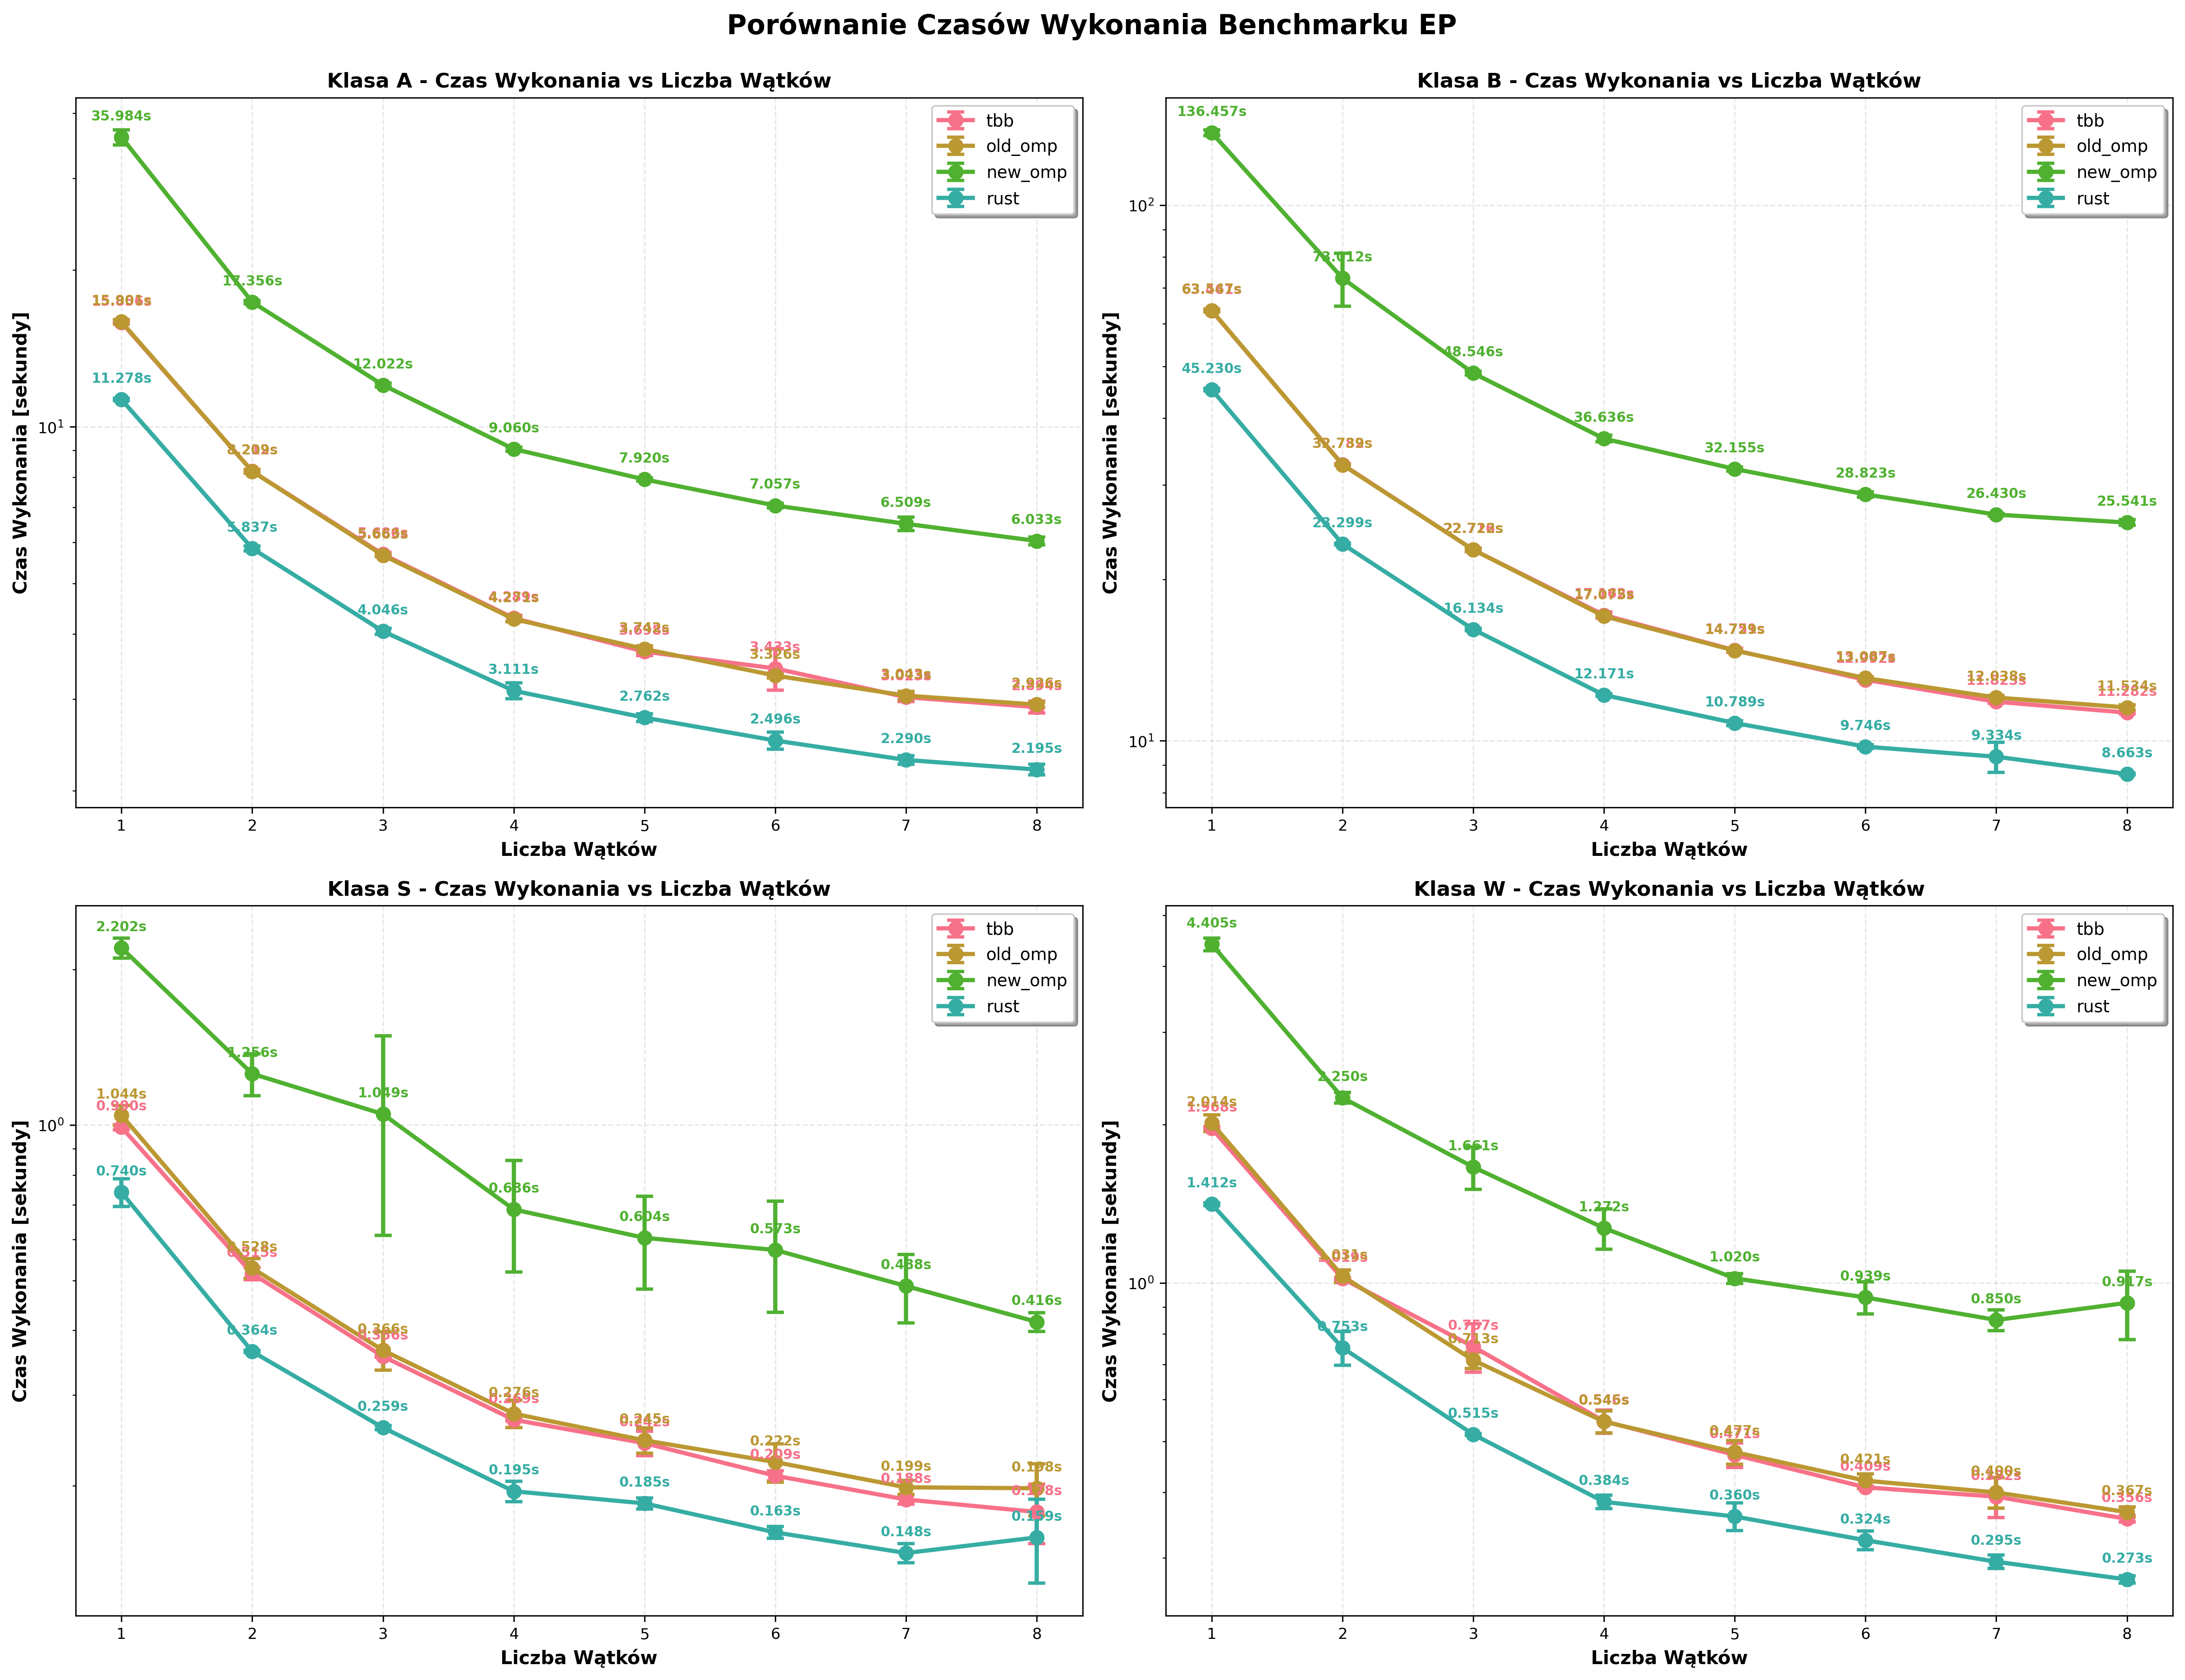
\includegraphics[width=0.9\textwidth]{analiza/images/parallel/ep/arm/ep_porownanie_czasow_wykonania.png}
    \caption{Porównanie czasów wykonania benchmarku EP dla klas S, W, A, B względem liczby użytych wątków}
    \label{ep_porownanie_czasow_wykonania}
\end{figure}

Na rysunku \ref{ep_porownanie_czasow_wykonania} zaprezentowano zestawienie czasów wykonania benchmarku EP dla czterech klas problemu: S, W, A oraz B, przy użyciu czterech różnych implementacji równoległości: TBB, OpenMP w wersji oryginalnej w stylu języka Fortran (\texttt{old\_omp}), OpenMP w wersji nowszej (\texttt{new\_omp}) oraz implementacji w języku Rust. Dla każdej z klas przedstawiono zależność czasu wykonania od liczby wątków (od 1 do 8). Wartości zostały zaprezentowane w skali logarytmicznej.

\begin{figure}[H]
    \centering
    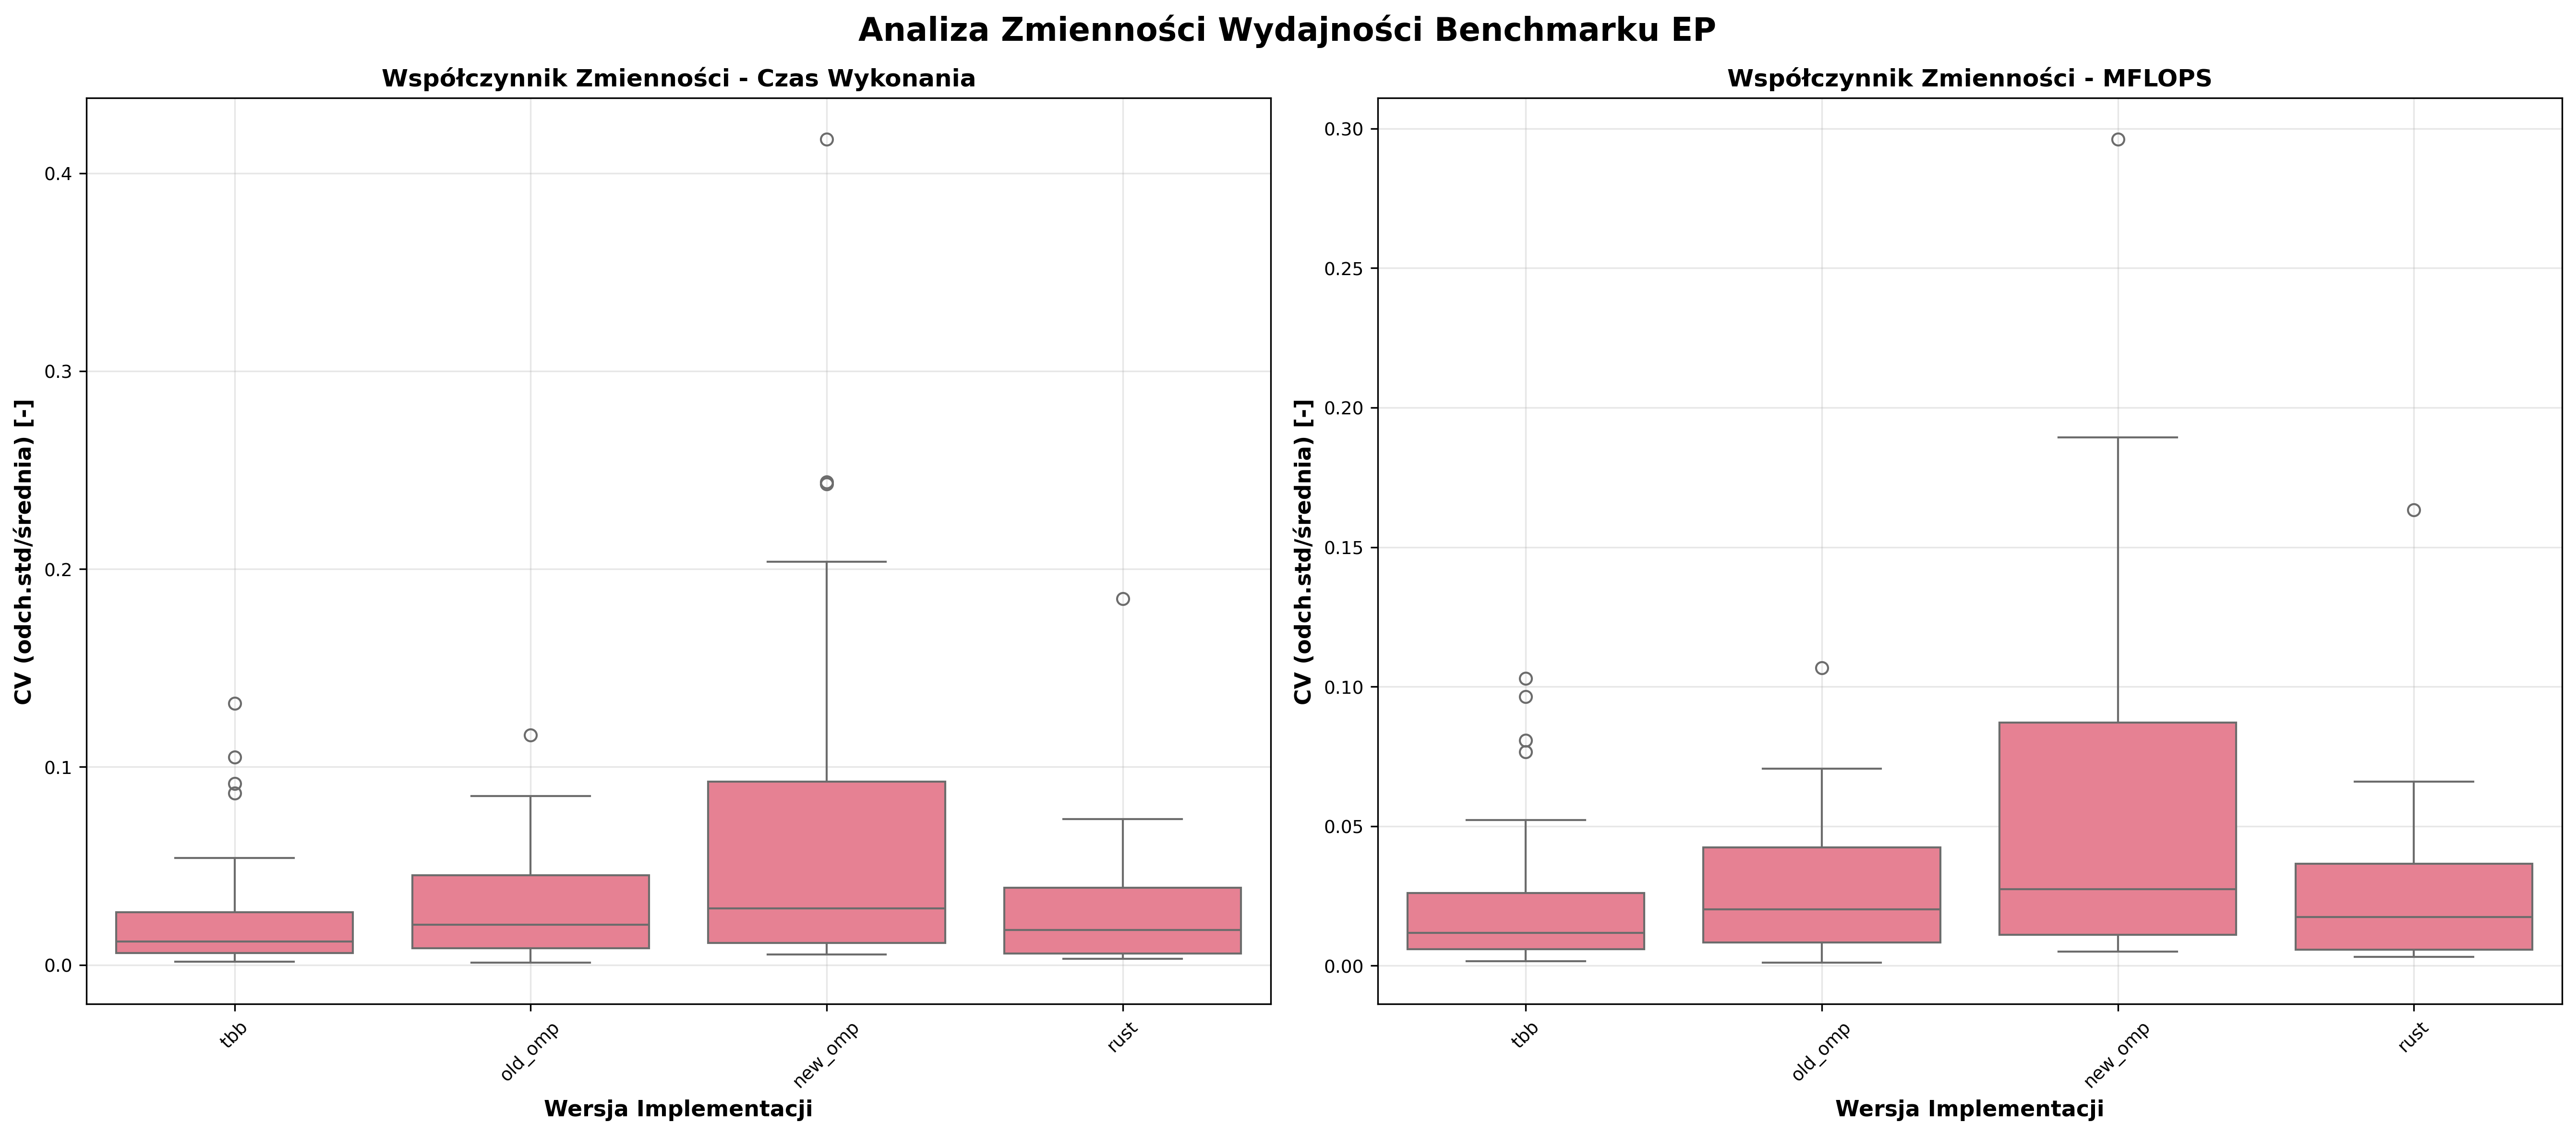
\includegraphics[width=0.9\textwidth]{analiza/images/parallel/ep/arm/ep_analiza_zmiennosci.png}
    \caption{Analiza zmienności czasów wykonania benchmarku EP dla klas S, W, A, B względem liczby użytych wątków}
    \label{ep_analiza_zmiennosci}
\end{figure}

Najlepsze rezultaty czasowe, niezależnie od klasy problemu, osiąga implementacja z użyciem języka Rust, co może świadczyć o wysokiej wydajności systemu wykonawczego tej technologii oraz efektywnej optymalizacji niskopoziomowej. \texttt{rust} wykazuje też największą stabilność czasową przy wzroście liczby wątków, co może sugerować niskie koszty narzutu zarządzania wątkami.

Zarówno \texttt{old\_omp}, jak i biblioteka TBB wykazują porównywalną wydajność w większości przypadków, przy czym TBB w klasach mniejszych (S, W) może osiągać nieco lepsze rezultaty, podczas gdy w klasach większych (A, B) ich wyniki się zbliżają. \texttt{new\_omp} cechuje się natomiast najgorszą skalowalnością i najdłuższymi czasami wykonania, co może wskazywać na mniej efektywną implementację zarządzania zadaniami równoległymi lub wyższy narzut synchronizacji.

W przypadku klasy B, ze względu na większą złożoność obliczeniową, czasy wykonania są znacząco dłuższe, a różnice pomiędzy bibliotekami bardziej wyraźne. Zastosowanie skali logarytmicznej w tej klasie dodatkowo uwypukla przewagę rozwiązań o lepszej skalowalności. Warto również zauważyć, że dla większej liczby wątków (6-8) część implementacji przestaje zyskiwać znacząco na wydajności.

\subsubsection{Zmienność czasu wykonania}
Na podstawie lewego wykresu - rysunek \ref{ep_analiza_zmiennosci} można zauważyć, że najniższą zmiennością czasów wykonania charakteryzują się implementacje oparte na bibliotekach TBB oraz Rust, co świadczy o ich dużej powtarzalności i deterministycznym charakterze działania. Mediany współczynnika zmienności dla tych implementacji pozostają na bardzo niskim poziomie, a obserwowane wartości odstające są rzadkie i relatywnie niewielkie.

Oryginalna wersja OpenMP również wykazuje dobrą stabilność, choć z nieco większą rozpiętością wyników niż TBB i Rust. Natomiast nowa wersja OpenMP prezentuje największą zmienność. Występowanie licznych wartości odstających oraz szeroki rozrzut wyników podkreślają potencjalną niestabilność tej wersji w testowanych warunkach.

\subsubsection{Zmienność MFLOPS}
Podobne zależności można zaobserwować na prawym wykresie - rysunek \ref{ep_analiza_zmiennosci}, przedstawiającym zmienność wartości MFLOPS. Tutaj również TBB oraz Rust wyróżniają się najmniejszymi wartościami współczynnika zmienności, co potwierdza ich przewidywalność pod względem wydajności obliczeniowej. OpenMP w starszej wersji (\texttt{old\_omp}) cechuje się umiarkowaną zmiennością, natomiast nowa wersja OpenMP (\texttt{new\_omp}) ponownie odznacza się największą rozpiętością oraz medianą współczynnika zmienności, co może mieć negatywne implikacje dla zastosowań wymagających stabilnej wydajności.



%------------------------------
\begin{figure}[H]
    \centering
    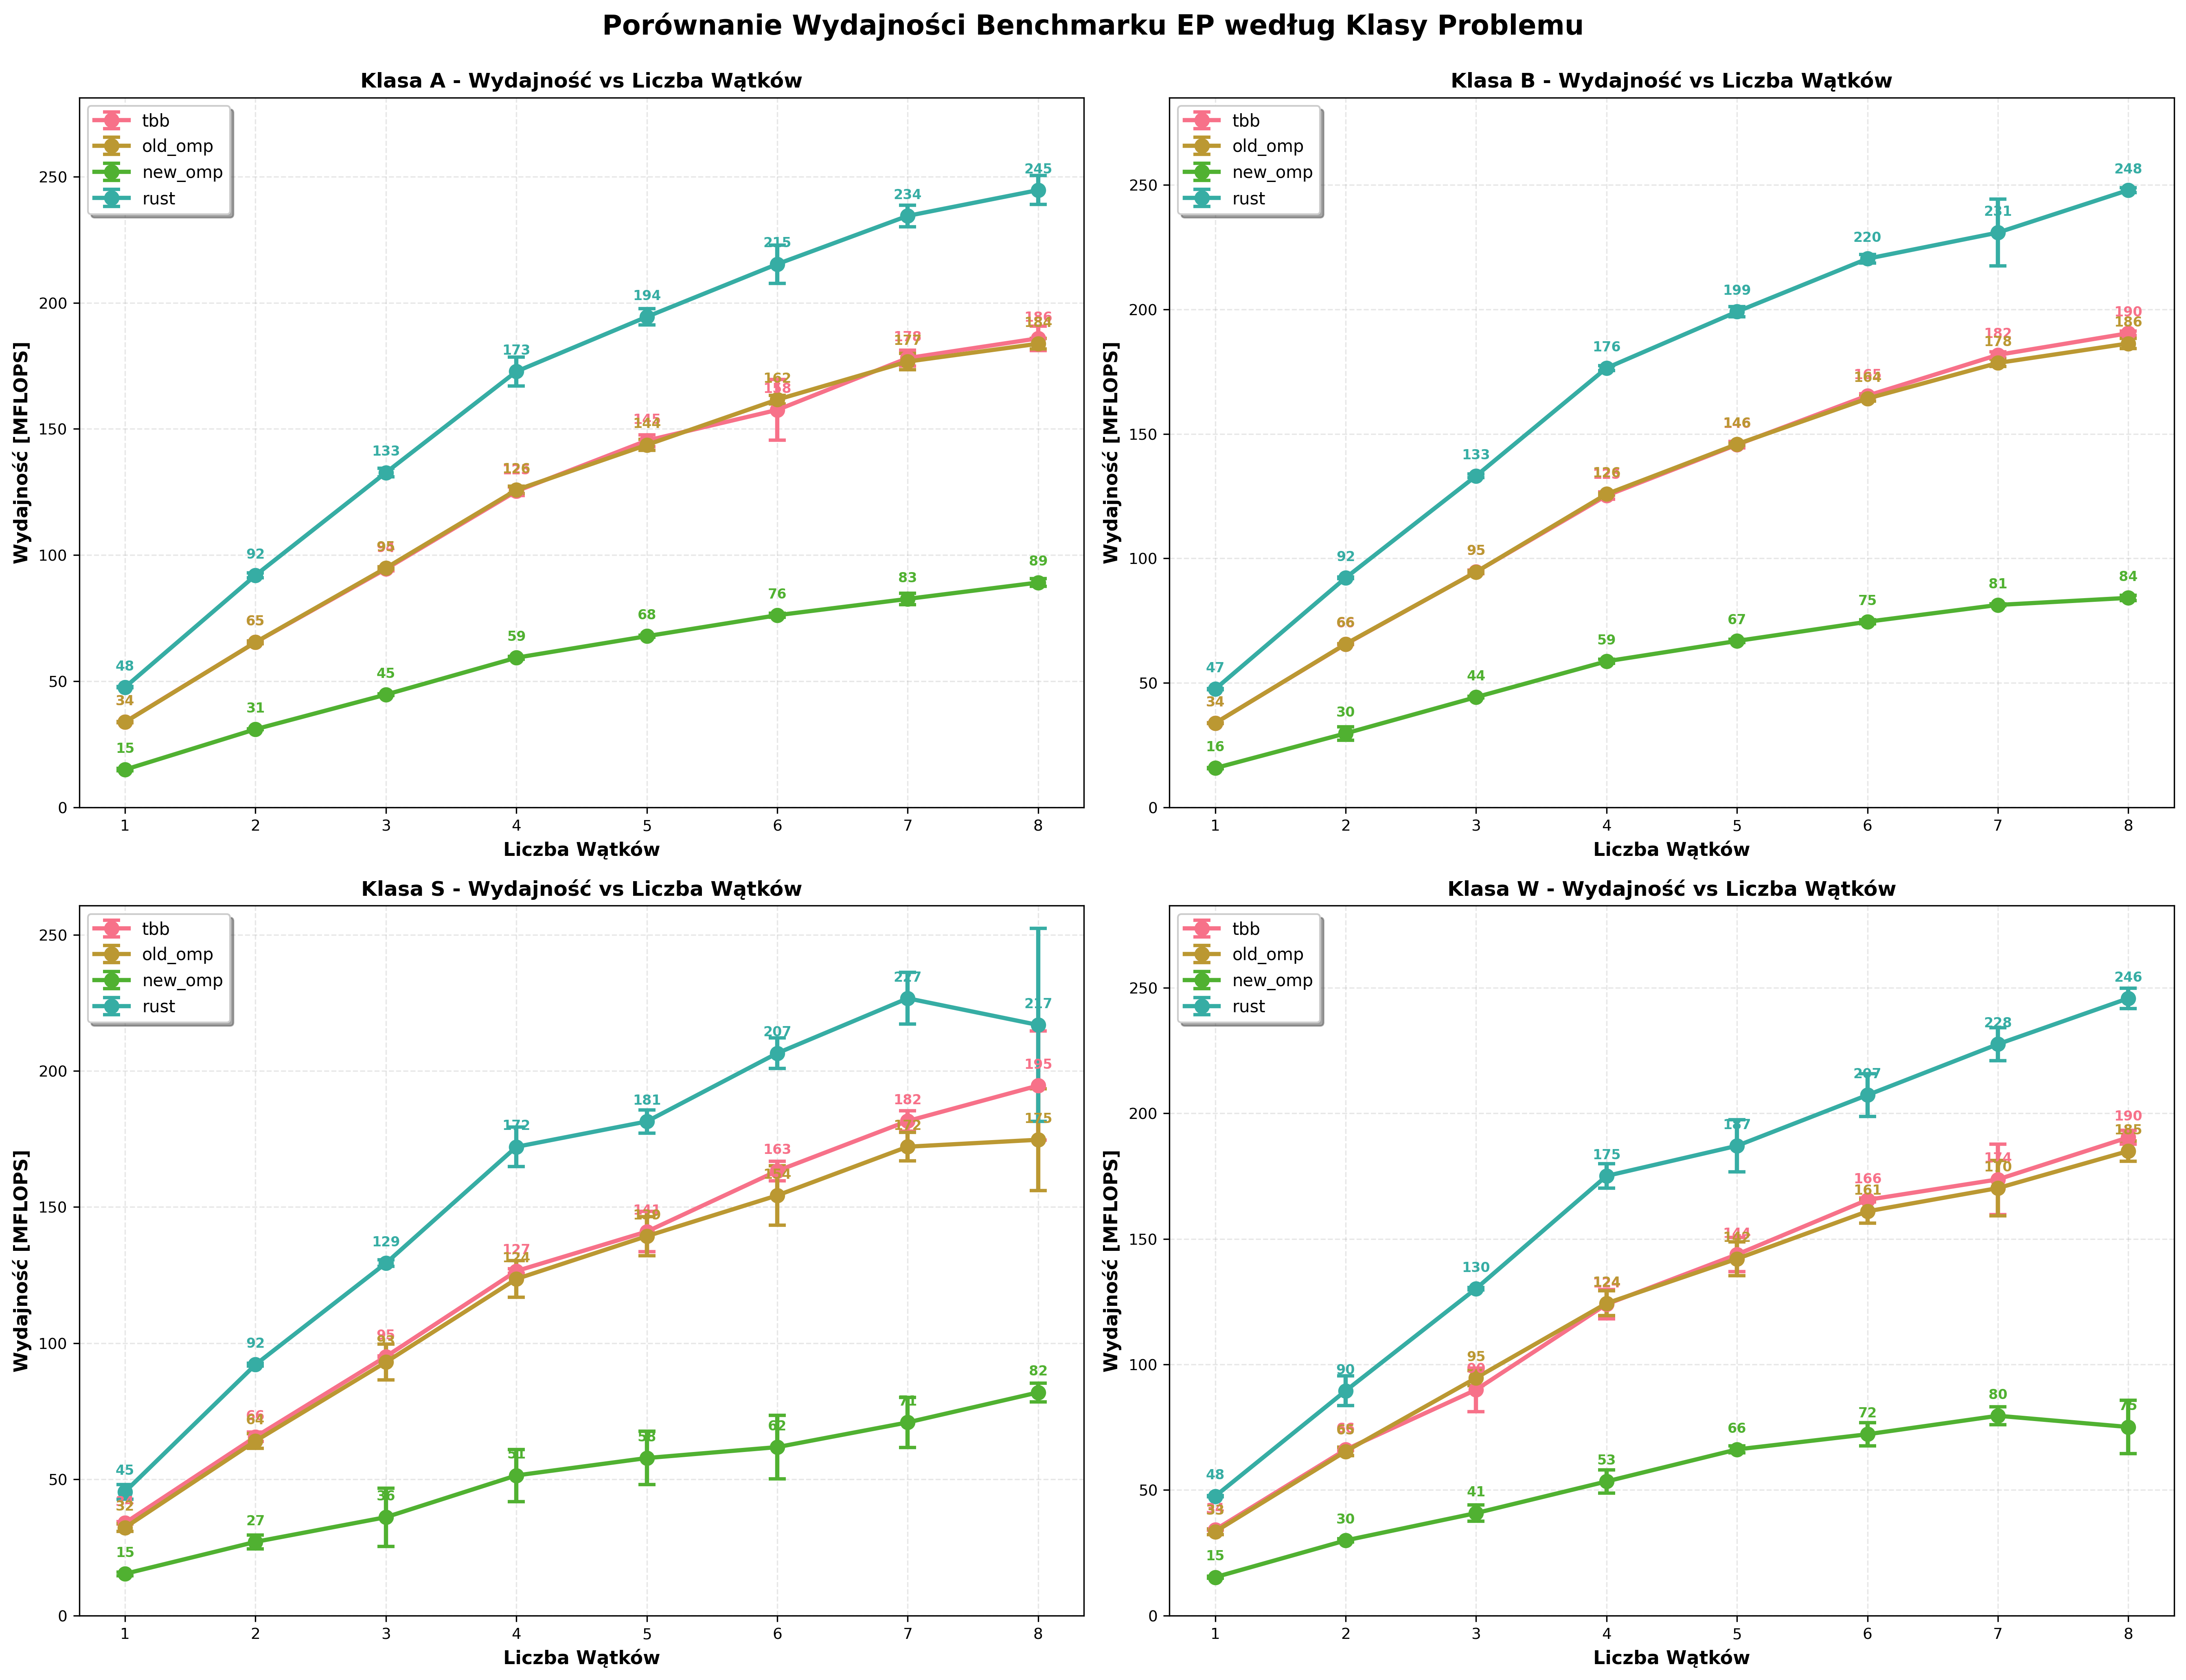
\includegraphics[width=0.9\textwidth]{analiza/images/parallel/ep/arm/ep_porownanie_wydajnosci.png}
    \caption{Porównanie wydajności benchmarku EP dla klas S, W, A, B względem liczby użytych wątków}
    \label{ep_porownanie_wydajnosci}
\end{figure}
Na wykresach na rysunku \ref{ep_porownanie_wydajnosci} zaprezentowano porównanie wydajności benchmarku EP mierzonej w MFLOPS (milionach operacji zmiennoprzecinkowych na sekundę). Wydajność została przedstawiona jako funkcja liczby wątków (1-8) dla czterech implementacji równoległych.

Implementacja w języku Rust konsekwentnie osiąga najwyższe wartości MFLOPS we wszystkich klasach problemu i dla każdej liczby wątków, co świadczy o bardzo efektywnym zarządzaniu równoległością oraz niskim narzucie wykonawczym. Warto również zauważyć, że \texttt{rust} uzyskuje szczególnie imponujące wyniki dla większej liczby wątków (6-8), gdzie inne implementacje wykazują tendencję do spowolnienia przyrostu wydajności.

Zarówno biblioteka TBB, jak i starsza wersja OpenMP osiągają zbliżoną wydajność i dobrą skalowalność. W większości przypadków wartości MFLOPS dla tych dwóch rozwiązań są porównywalne, przy czym TBB niekiedy uzyskuje nieco lepsze rezultaty, szczególnie dla klas S i~W.

Z kolei implementacja oparta na nowej wersji OpenMP wykazuje wyraźnie niższą wydajność w porównaniu z pozostałymi rozwiązaniami. Różnice te są szczególnie widoczne przy większej liczbie wątków, gdzie wzrost MFLOPS jest bardziej spłaszczony, co może wskazywać na ograniczenia w mechanizmach planowania zadań lub zwiększony narzut synchronizacji.


\begin{figure}[H]
    \centering
    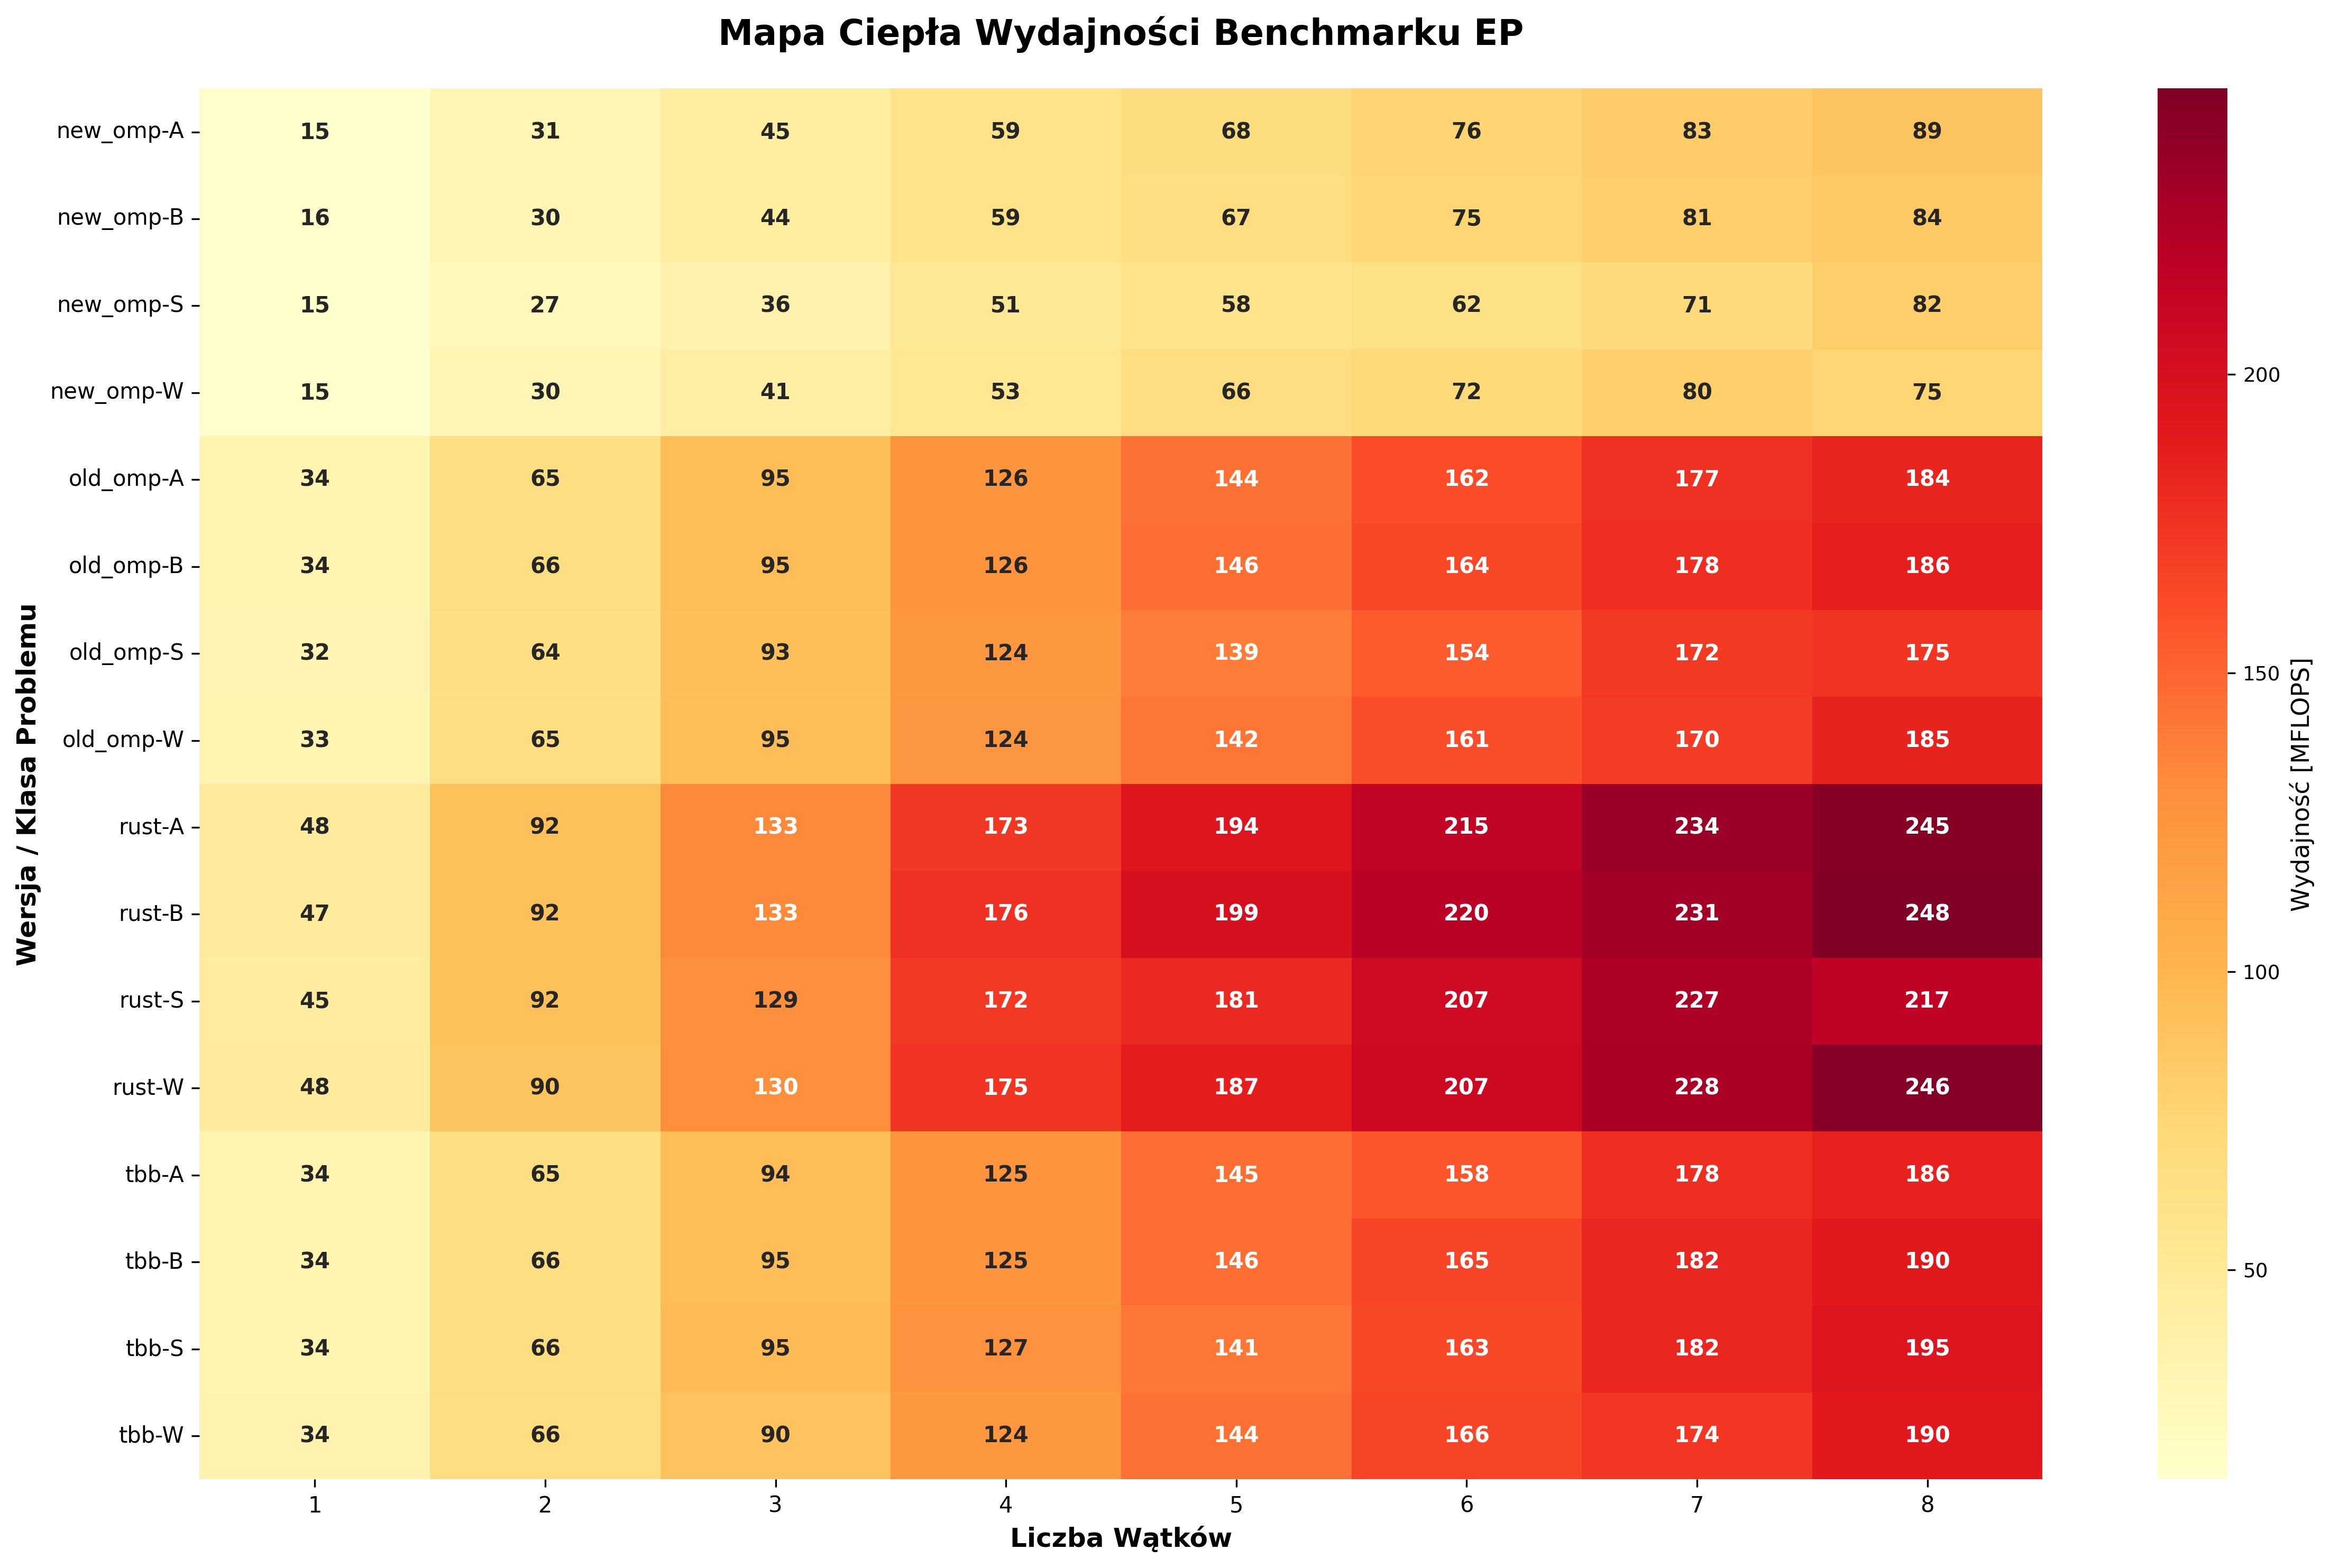
\includegraphics[width=0.9\textwidth]{analiza/images/parallel/ep/arm/ep_mapa_ciepla_wydajnosci.png}
    \caption{Mapa ciepła wydajności benchmarku EP dla klas S, W, A, B względem liczby użytych wątków}
    \label{ep_heatmap_wydajnosci}
\end{figure}
Powyższa mapa cieplna - rysunek \ref{ep_heatmap_wydajnosci} przedstawia wydajność (w MFLOPS). Wydajność została przedstawiona w zależności od liczby użytych wątków. Odcienie koloru od żółtego do ciemnoczerwonego wskazują na wzrost wydajności.\\
Mapa ciepła jednoznacznie potwierdza przewagę implementacji \texttt{rust} w każdym układzie: dla wszystkich klas problemu i liczby wątków. Wartości MFLOPS przekraczające 240 dla 8 wątków (np. 248 MFLOPS dla klasy B) są wyraźnie wyższe od wyników pozostałych bibliotek, w~których wartości maksymalne oscylują w okolicach 185-195 MFLOPS.



\begin{figure}[H]
    \centering
    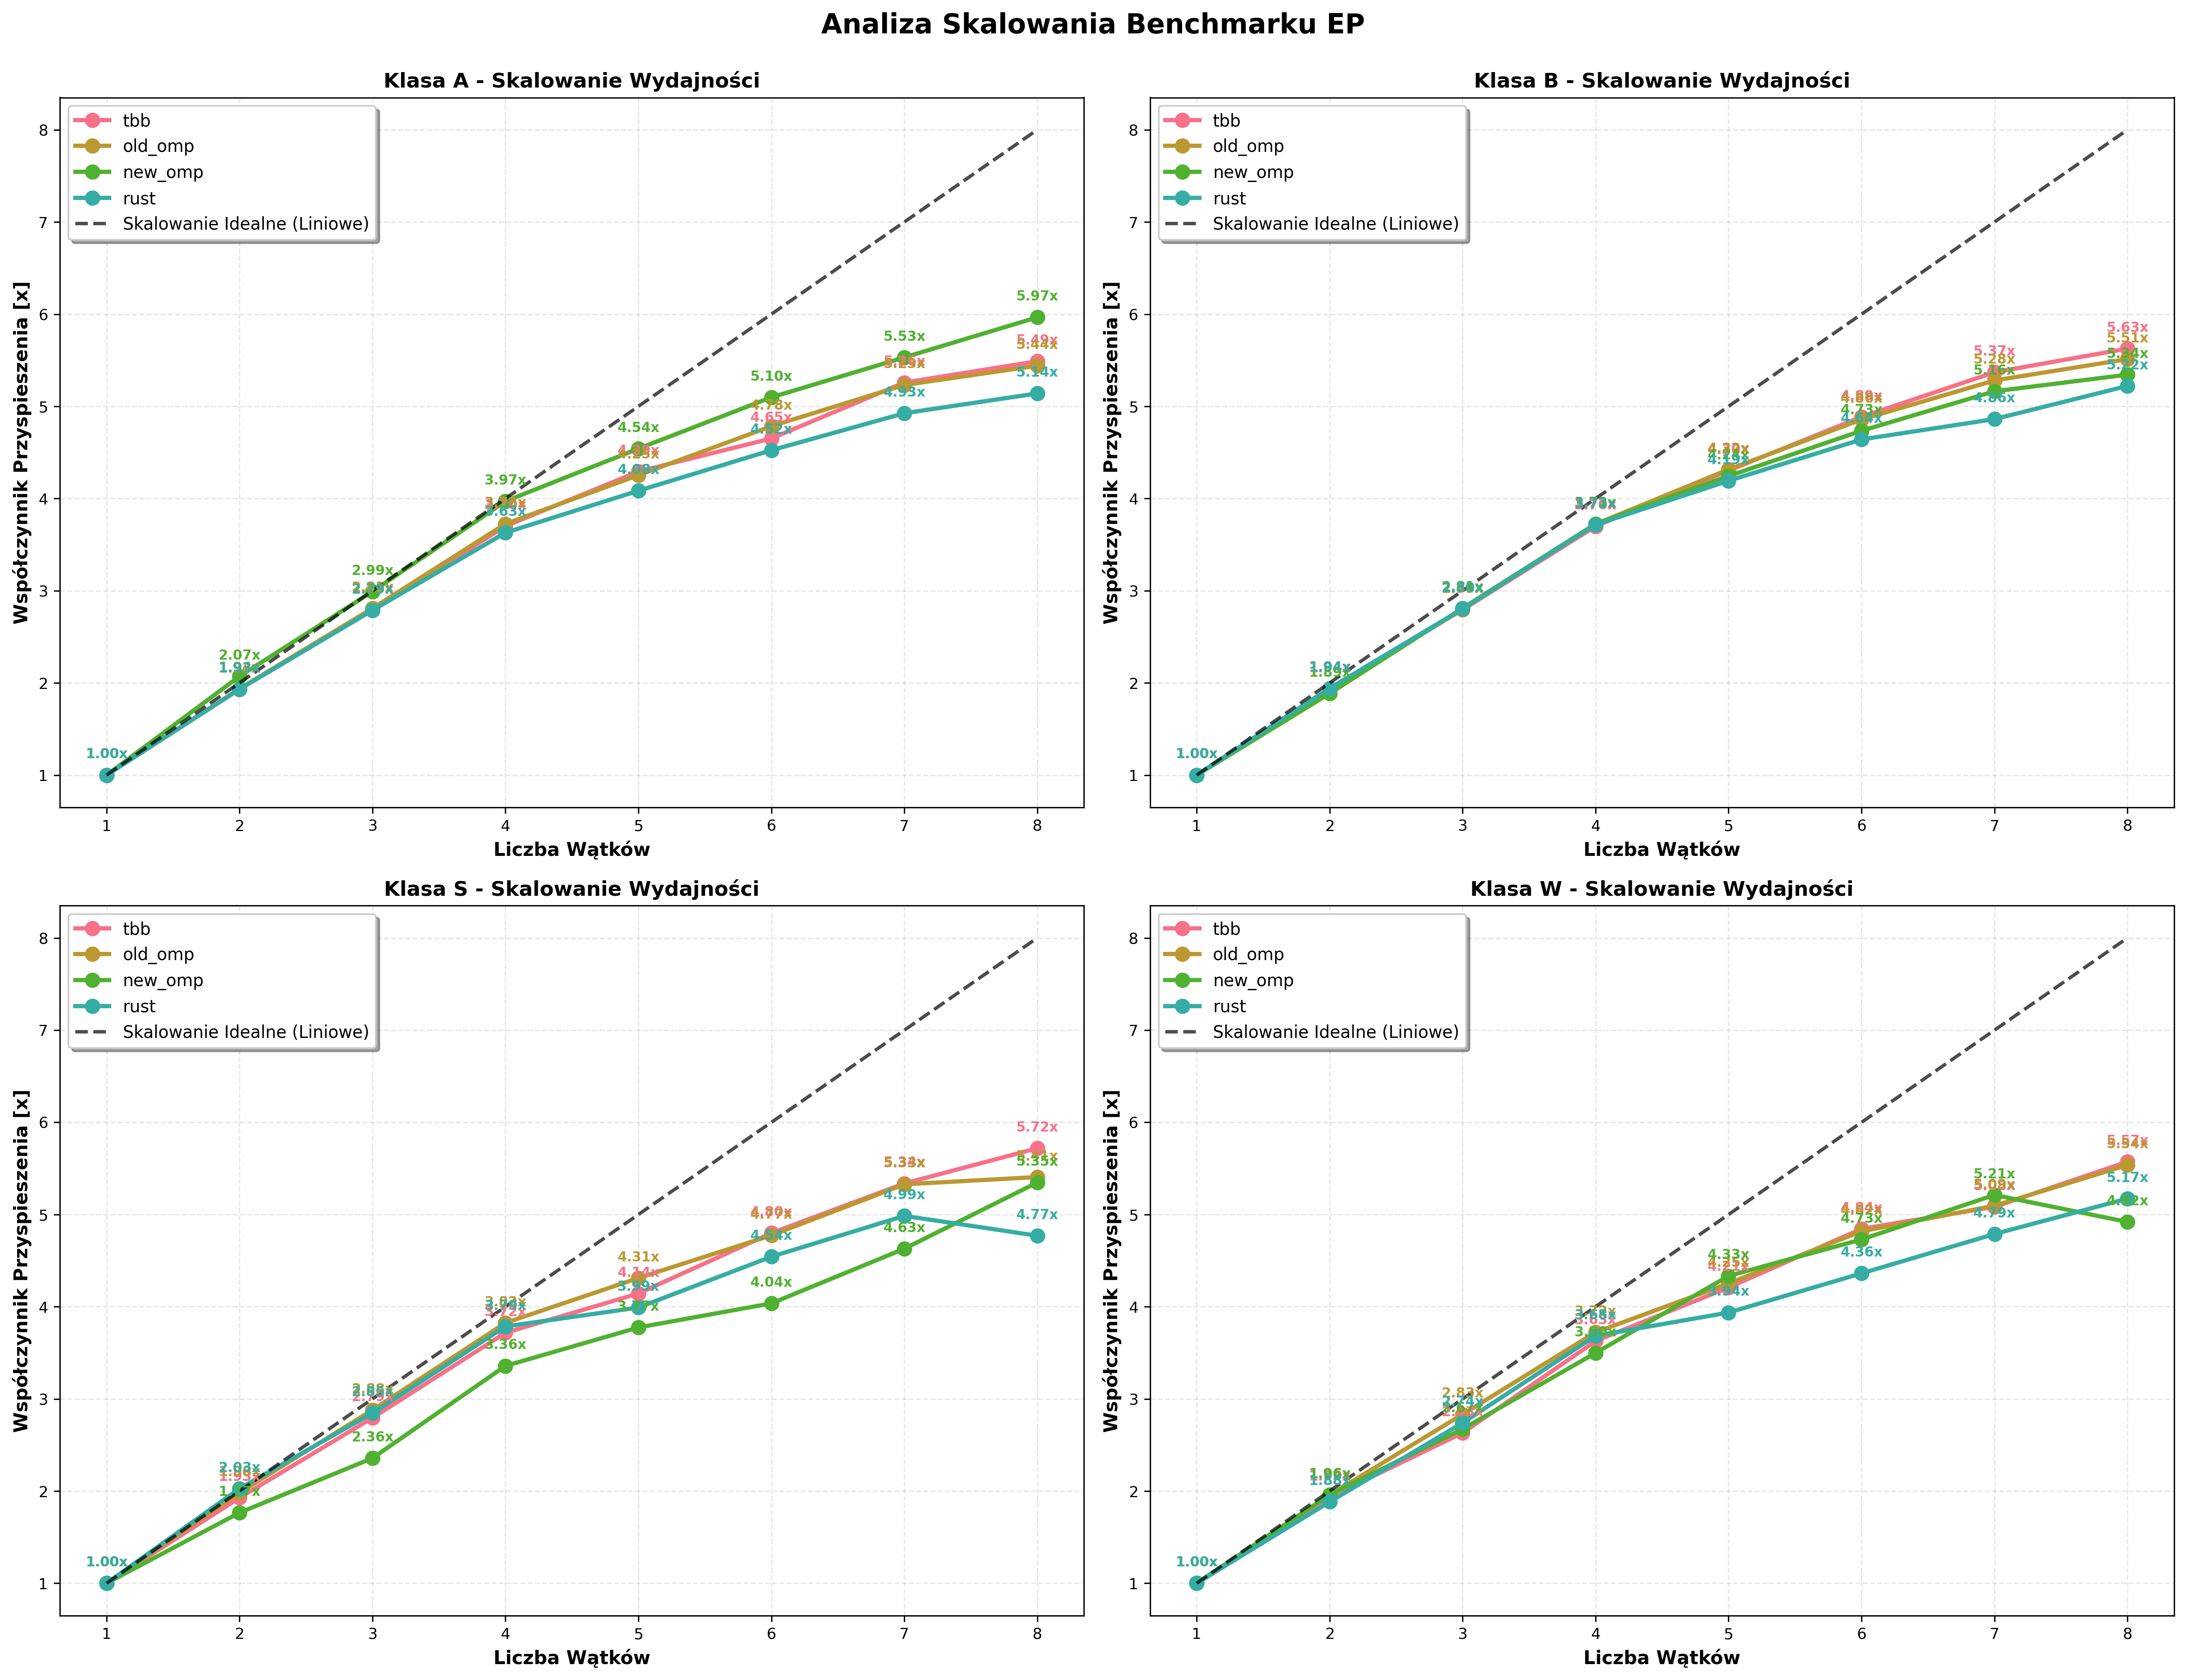
\includegraphics[width=0.9\textwidth]{analiza/images/parallel/ep/arm/ep_analiza_skalowania.png}
    \caption{Analiza skalowania benchmarku EP dla klas S, W, A, B względem liczby użytych wątków}
    \label{ep_analiza_skalowania}
\end{figure}
Powyższy wykres - rysunek \ref{ep_analiza_skalowania} przedstawia skalowanie wydajności benchmarku EP. Skalowanie wyrażone zostało za pomocą współczynnika przyspieszenia względem wykonania jednowątkowego i odniesione do skalowania idealnego (liniowego).

Spośród analizowanych implementacji \texttt{tbb} konsekwentnie osiąga najwyższe przyspieszenie we wszystkich klasach, najbardziej zbliżając się do idealnej skalowalności liniowej. Na drugim miejscu plasuje się \texttt{old\_omp}, które wykazuje stabilne, choć nieco niższe wyniki w porównaniu do \texttt{tbb}. New\_omp uzyskuje przyspieszenie niższe od \texttt{old\_omp}, ale wyższe od \texttt{rust}, która w~każdej klasie osiąga najniższe wartości. Przykładowo, dla ośmiu wątków w klasie A \texttt{tbb} osiąga przyspieszenie rzędu 5,97x, podczas gdy \texttt{rust} ogranicza się do 5,10x, co ilustruje wyraźną różnicę w wydajności.

Różnice między implementacjami stają się bardziej wyraźne przy większej liczbie wątków, co wskazuje na lepszą zdolność \texttt{tbb} i \texttt{old\_omp} do efektywnego wykorzystania równoległości w benchmarku EP. Subliniowy charakter skalowalności jest widoczny we wszystkich przypadkach, jednak \texttt{tbb} wykazuje najmniejsze odstępstwo od idealnego wzrostu, sugerując wyższą efektywność w zarządzaniu wątkami i minimalizacji narzutów.

\subsection{Wyniki benchmarków - platforma x86\_64}
\begin{figure}[H]
    \centering
    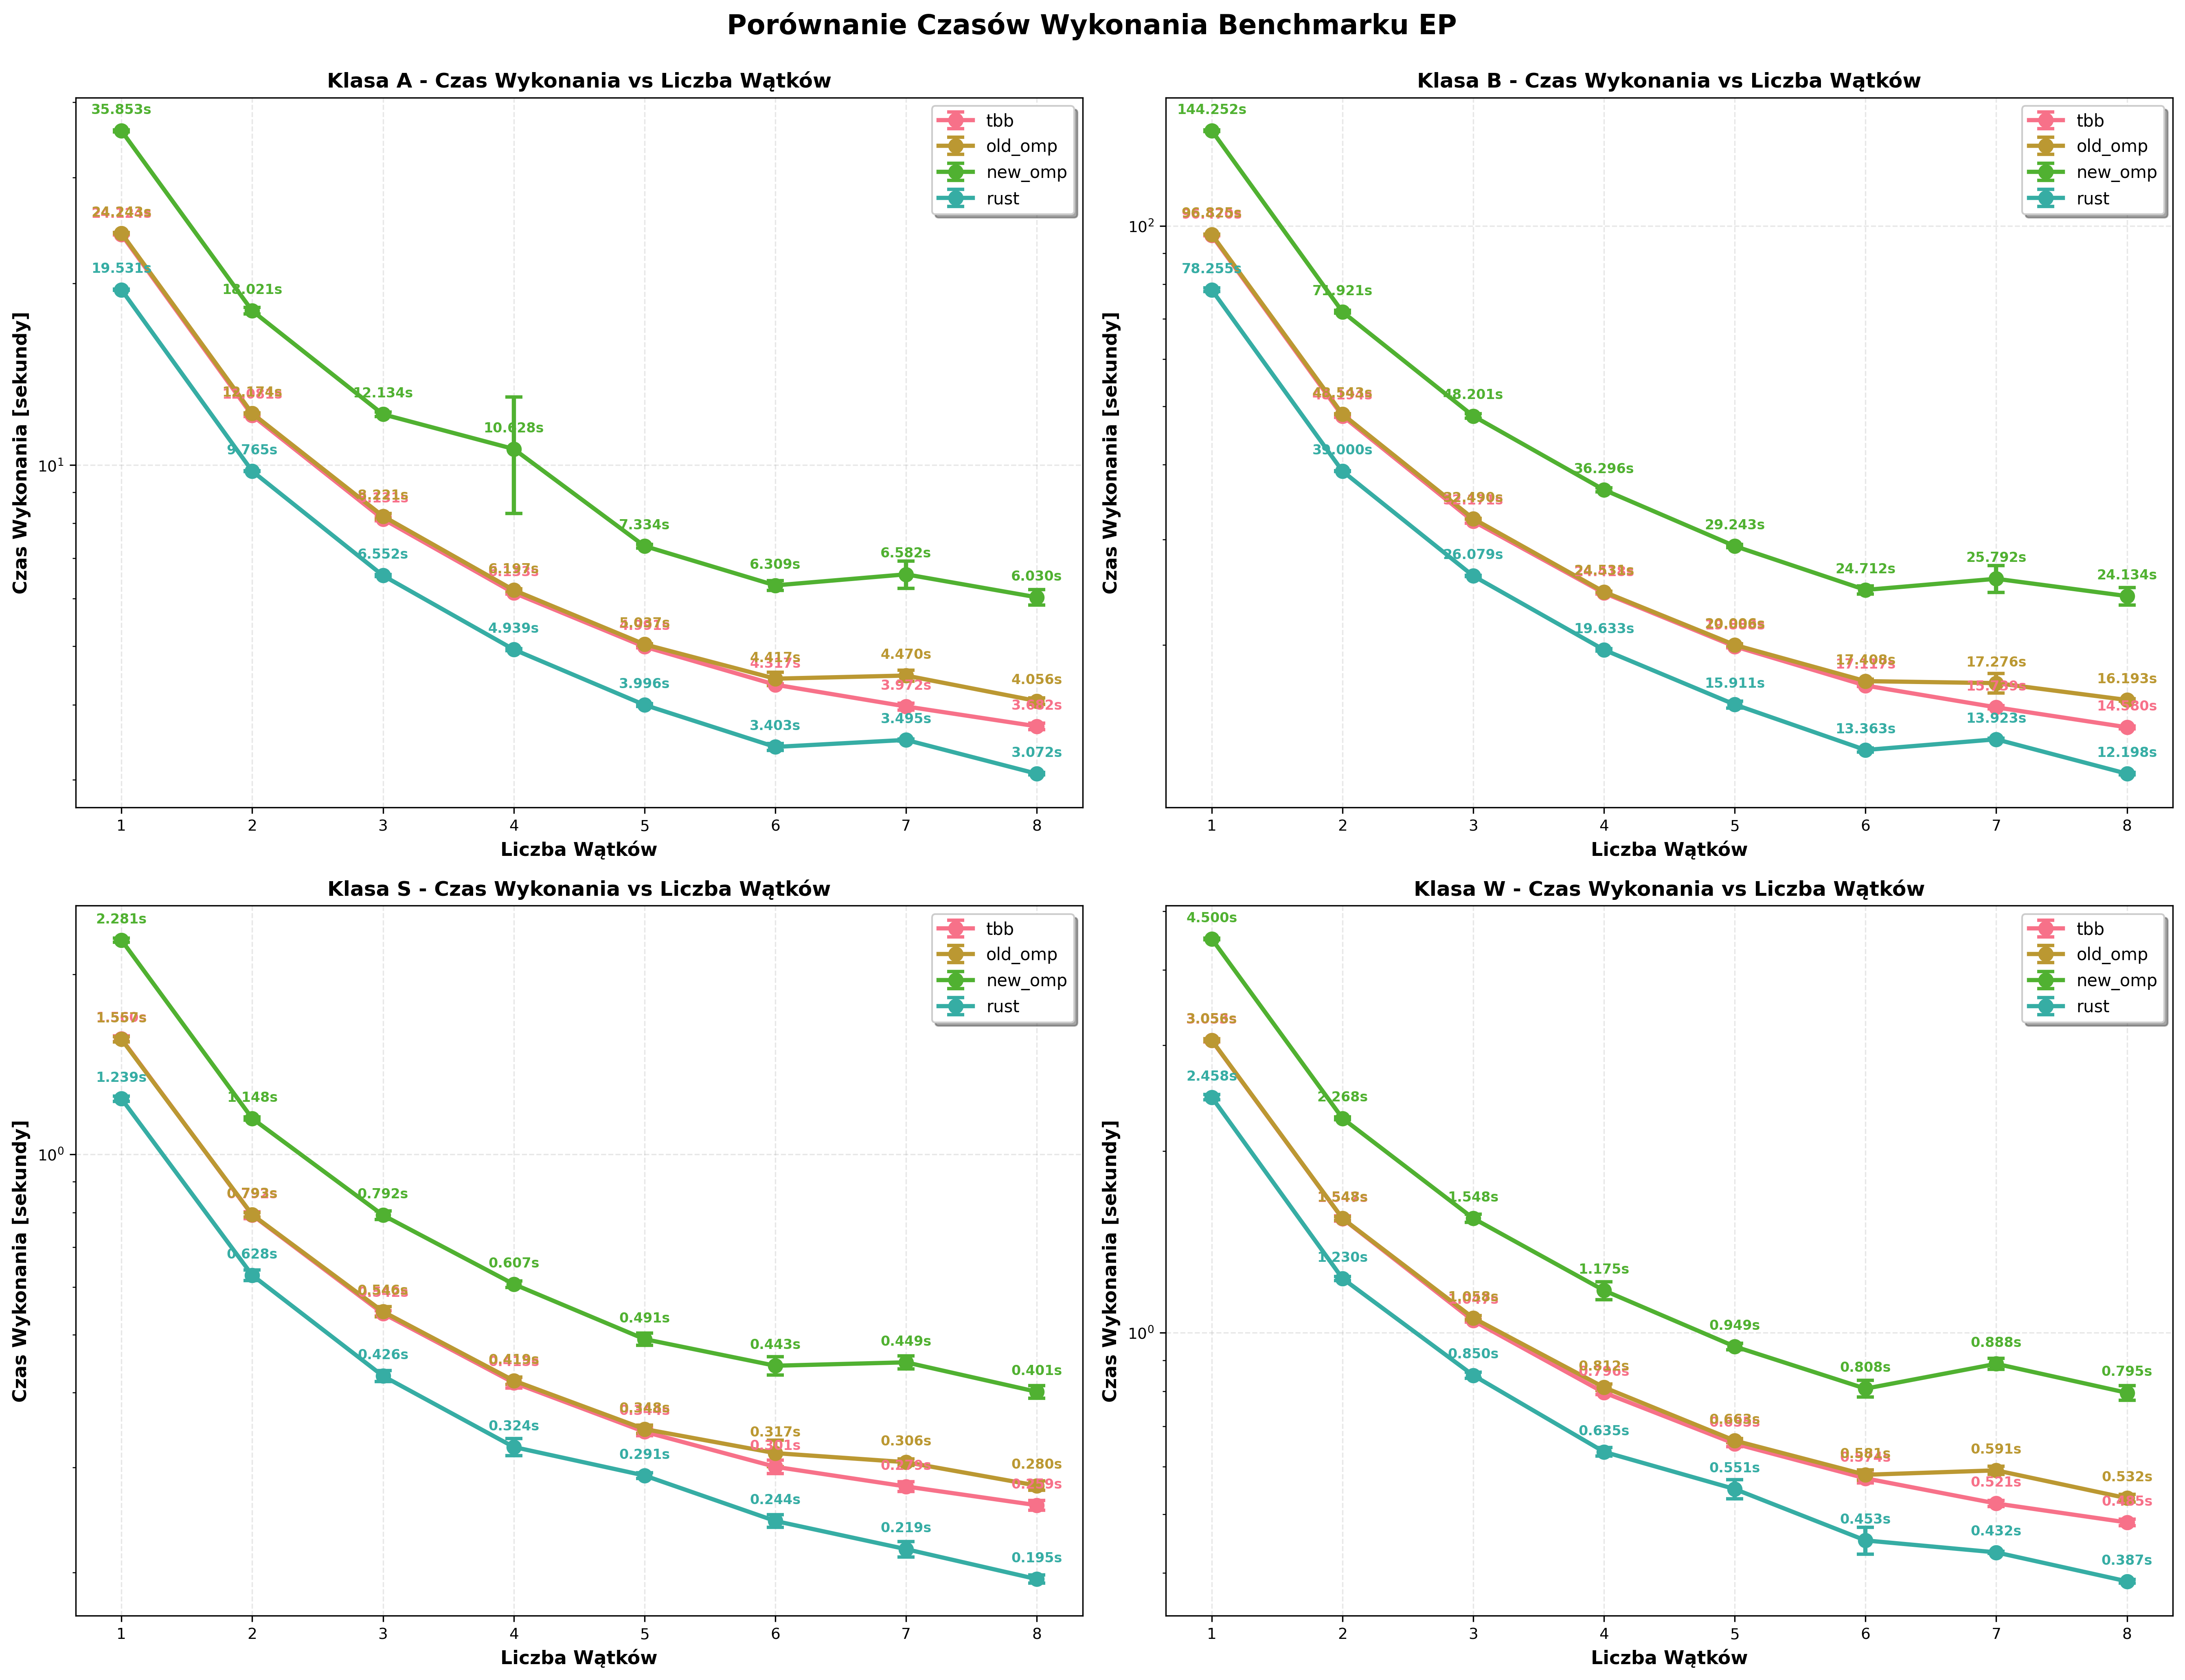
\includegraphics[width=0.9\textwidth]{analiza/images/parallel/ep/x86/ep_porownanie_czasow_wykonania.png}
    \caption{Porównanie czasów wykonania benchmarku EP dla klas S, W, A, B względem liczby użytych wątków}
    \label{ep_porownanie_czasow_wykonania_x86_64}
\end{figure}

\begin{figure}[H]
    \centering
    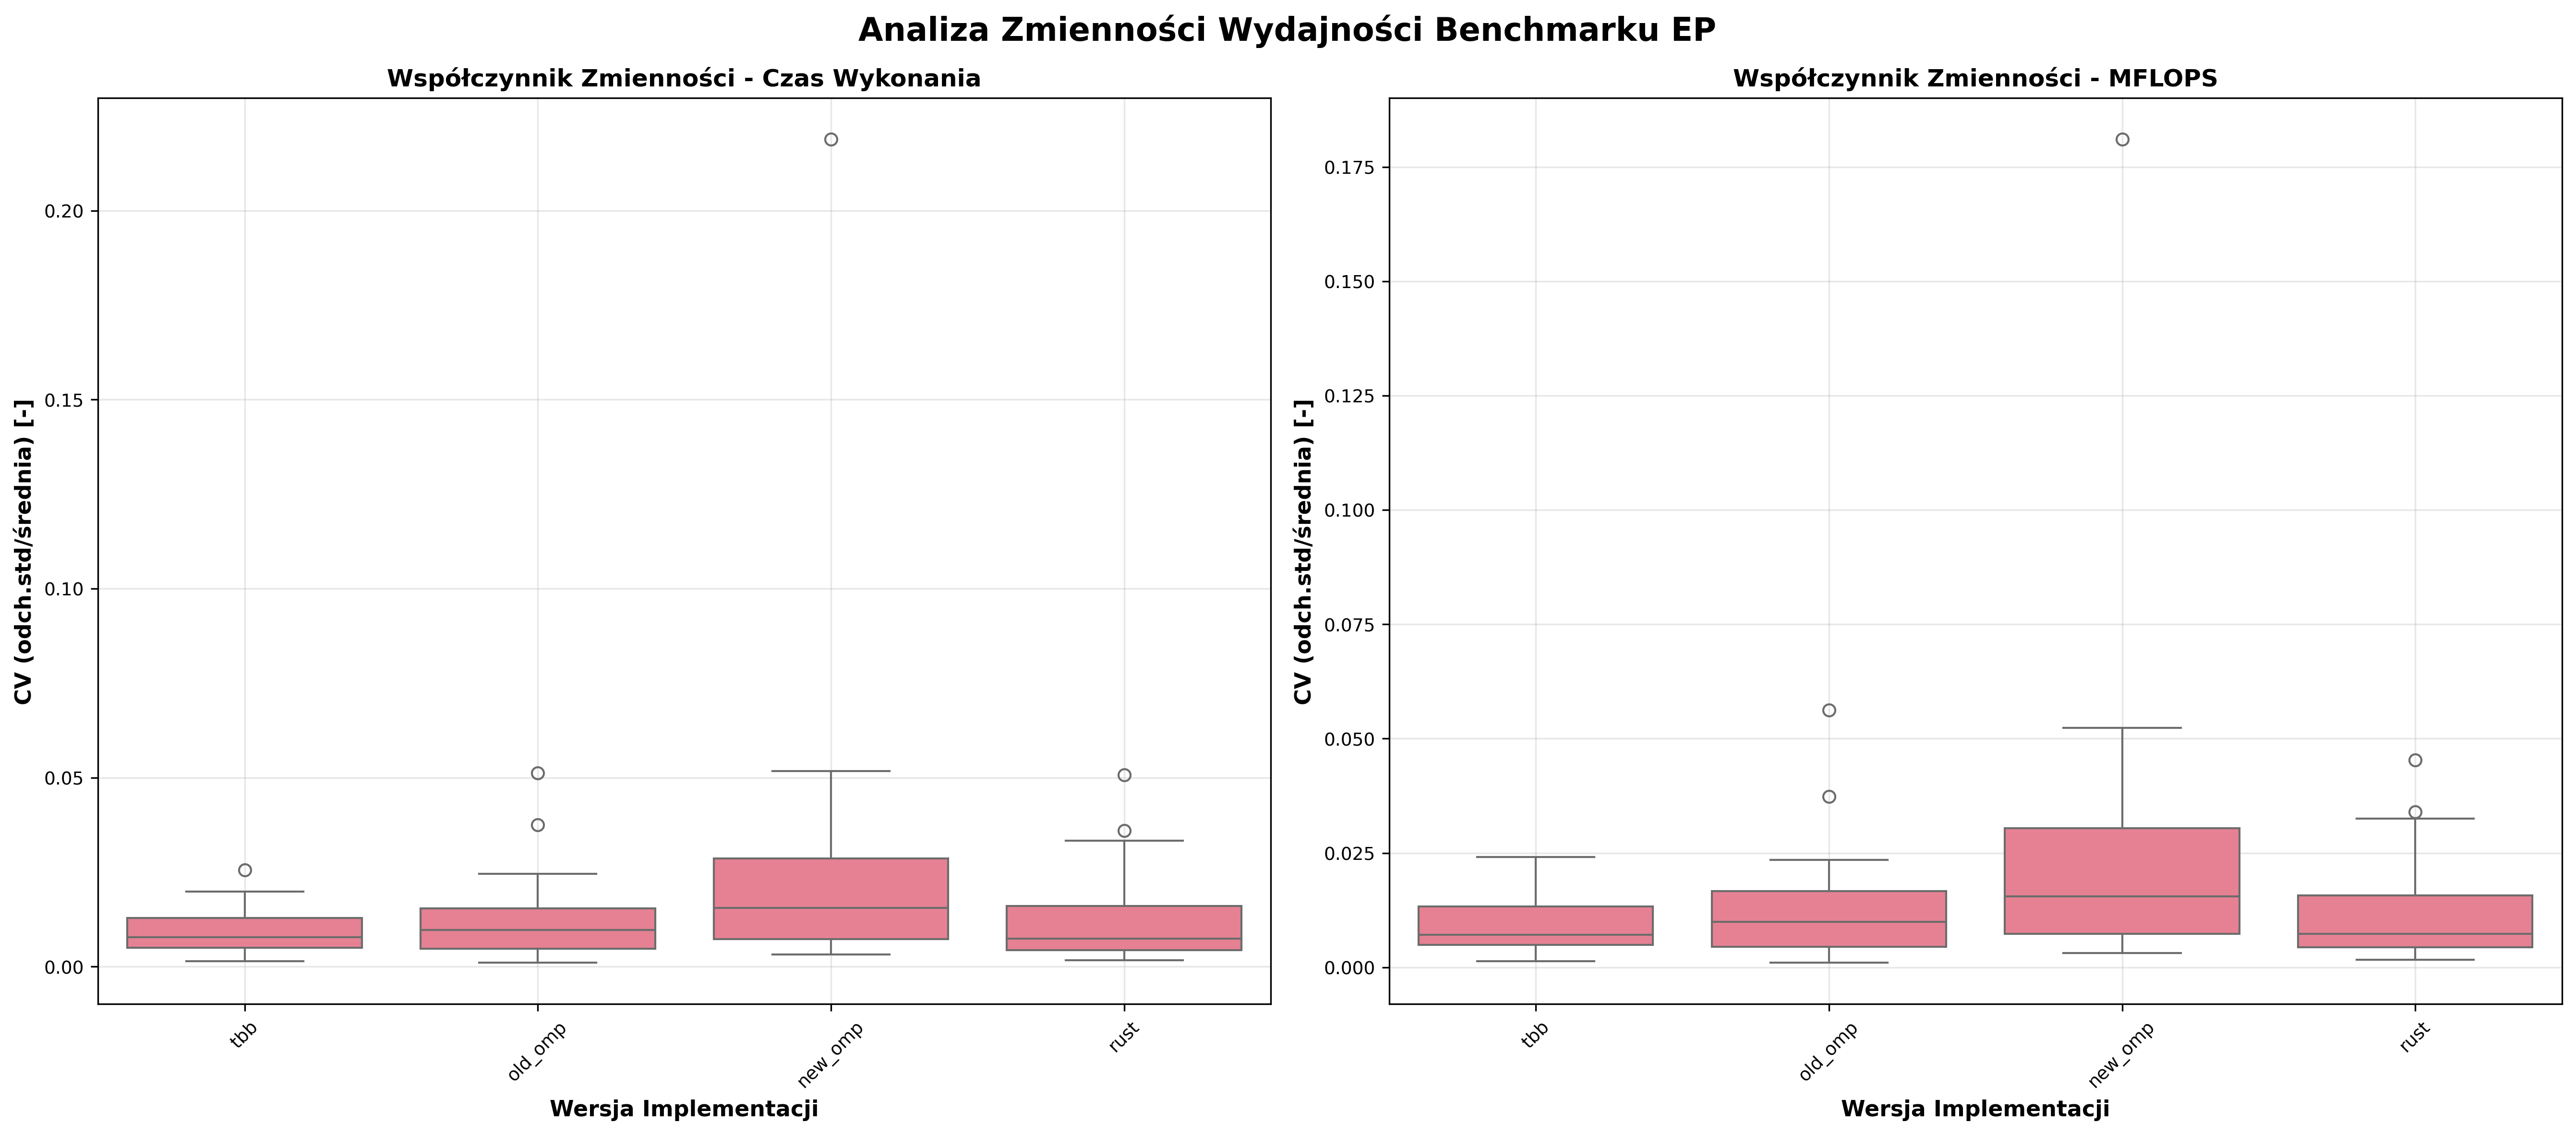
\includegraphics[width=0.9\textwidth]{analiza/images/parallel/ep/x86/ep_analiza_zmiennosci.png}
    \caption{Analiza zmienności czasów wykonania benchmarku EP dla klas S, W, A, B względem liczby użytych wątków}
    \label{ep_analiza_zmiennosci_x86_64}
\end{figure}

Analiza danych wskazuje, że implementacja \texttt{rust} konsekwentnie osiąga najniższe czasy wykonania przy maksymalnej liczbie wątków (8) we wszystkich klasach, co świadczy o jej wyższości w kontekście obliczeń równoległych.
W porównaniu do pozostałych implementacji, \texttt{rust} wykazuje zauważalną przewagę, szczególnie wyraźną w klasach S i W, gdzie różnice w czasach wykonania są bardziej znaczące. Implementacja ttb plasuje się na drugim miejscu pod względem wydajności, podczas gdy \texttt{old\_omp} i \texttt{new\_omp} charakteryzują się wyższymi czasami wykonania, z~\texttt{new\_omp} wykazującym najniższą efektywność.

Interpretując wykresy - rysunek \ref{ep_analiza_zmiennosci_x86_64}, można zauważyć, że dla wszystkich wersji implementacji wartości współczynnika zmienności są stosunkowo niskie, co oznacza wysoką powtarzalność i stabilność pomiarów. Najwyższą zmienność, zarówno dla czasu wykonania, jak i MFLOPS, obserwuje się w przypadku implementacji \texttt{new\_omp}, co sugeruje, że wyniki tej wersji są mniej stabilne w porównaniu do pozostałych. Implementacje \texttt{tbb}, \texttt{old\_omp} oraz \texttt{rust} charakteryzują się niższymi wartościami CV, co świadczy o większej niezawodności uzyskiwanych rezultatów.

Warto zwrócić uwagę na obecność pojedynczych punktów poza głównym zakresem wykresów, które mogą wskazywać na sporadyczne przypadki większych odchyleń w pomiarach, jednak nie wpływają one znacząco na ogólną ocenę stabilności.

\begin{figure}[H]
    \centering
    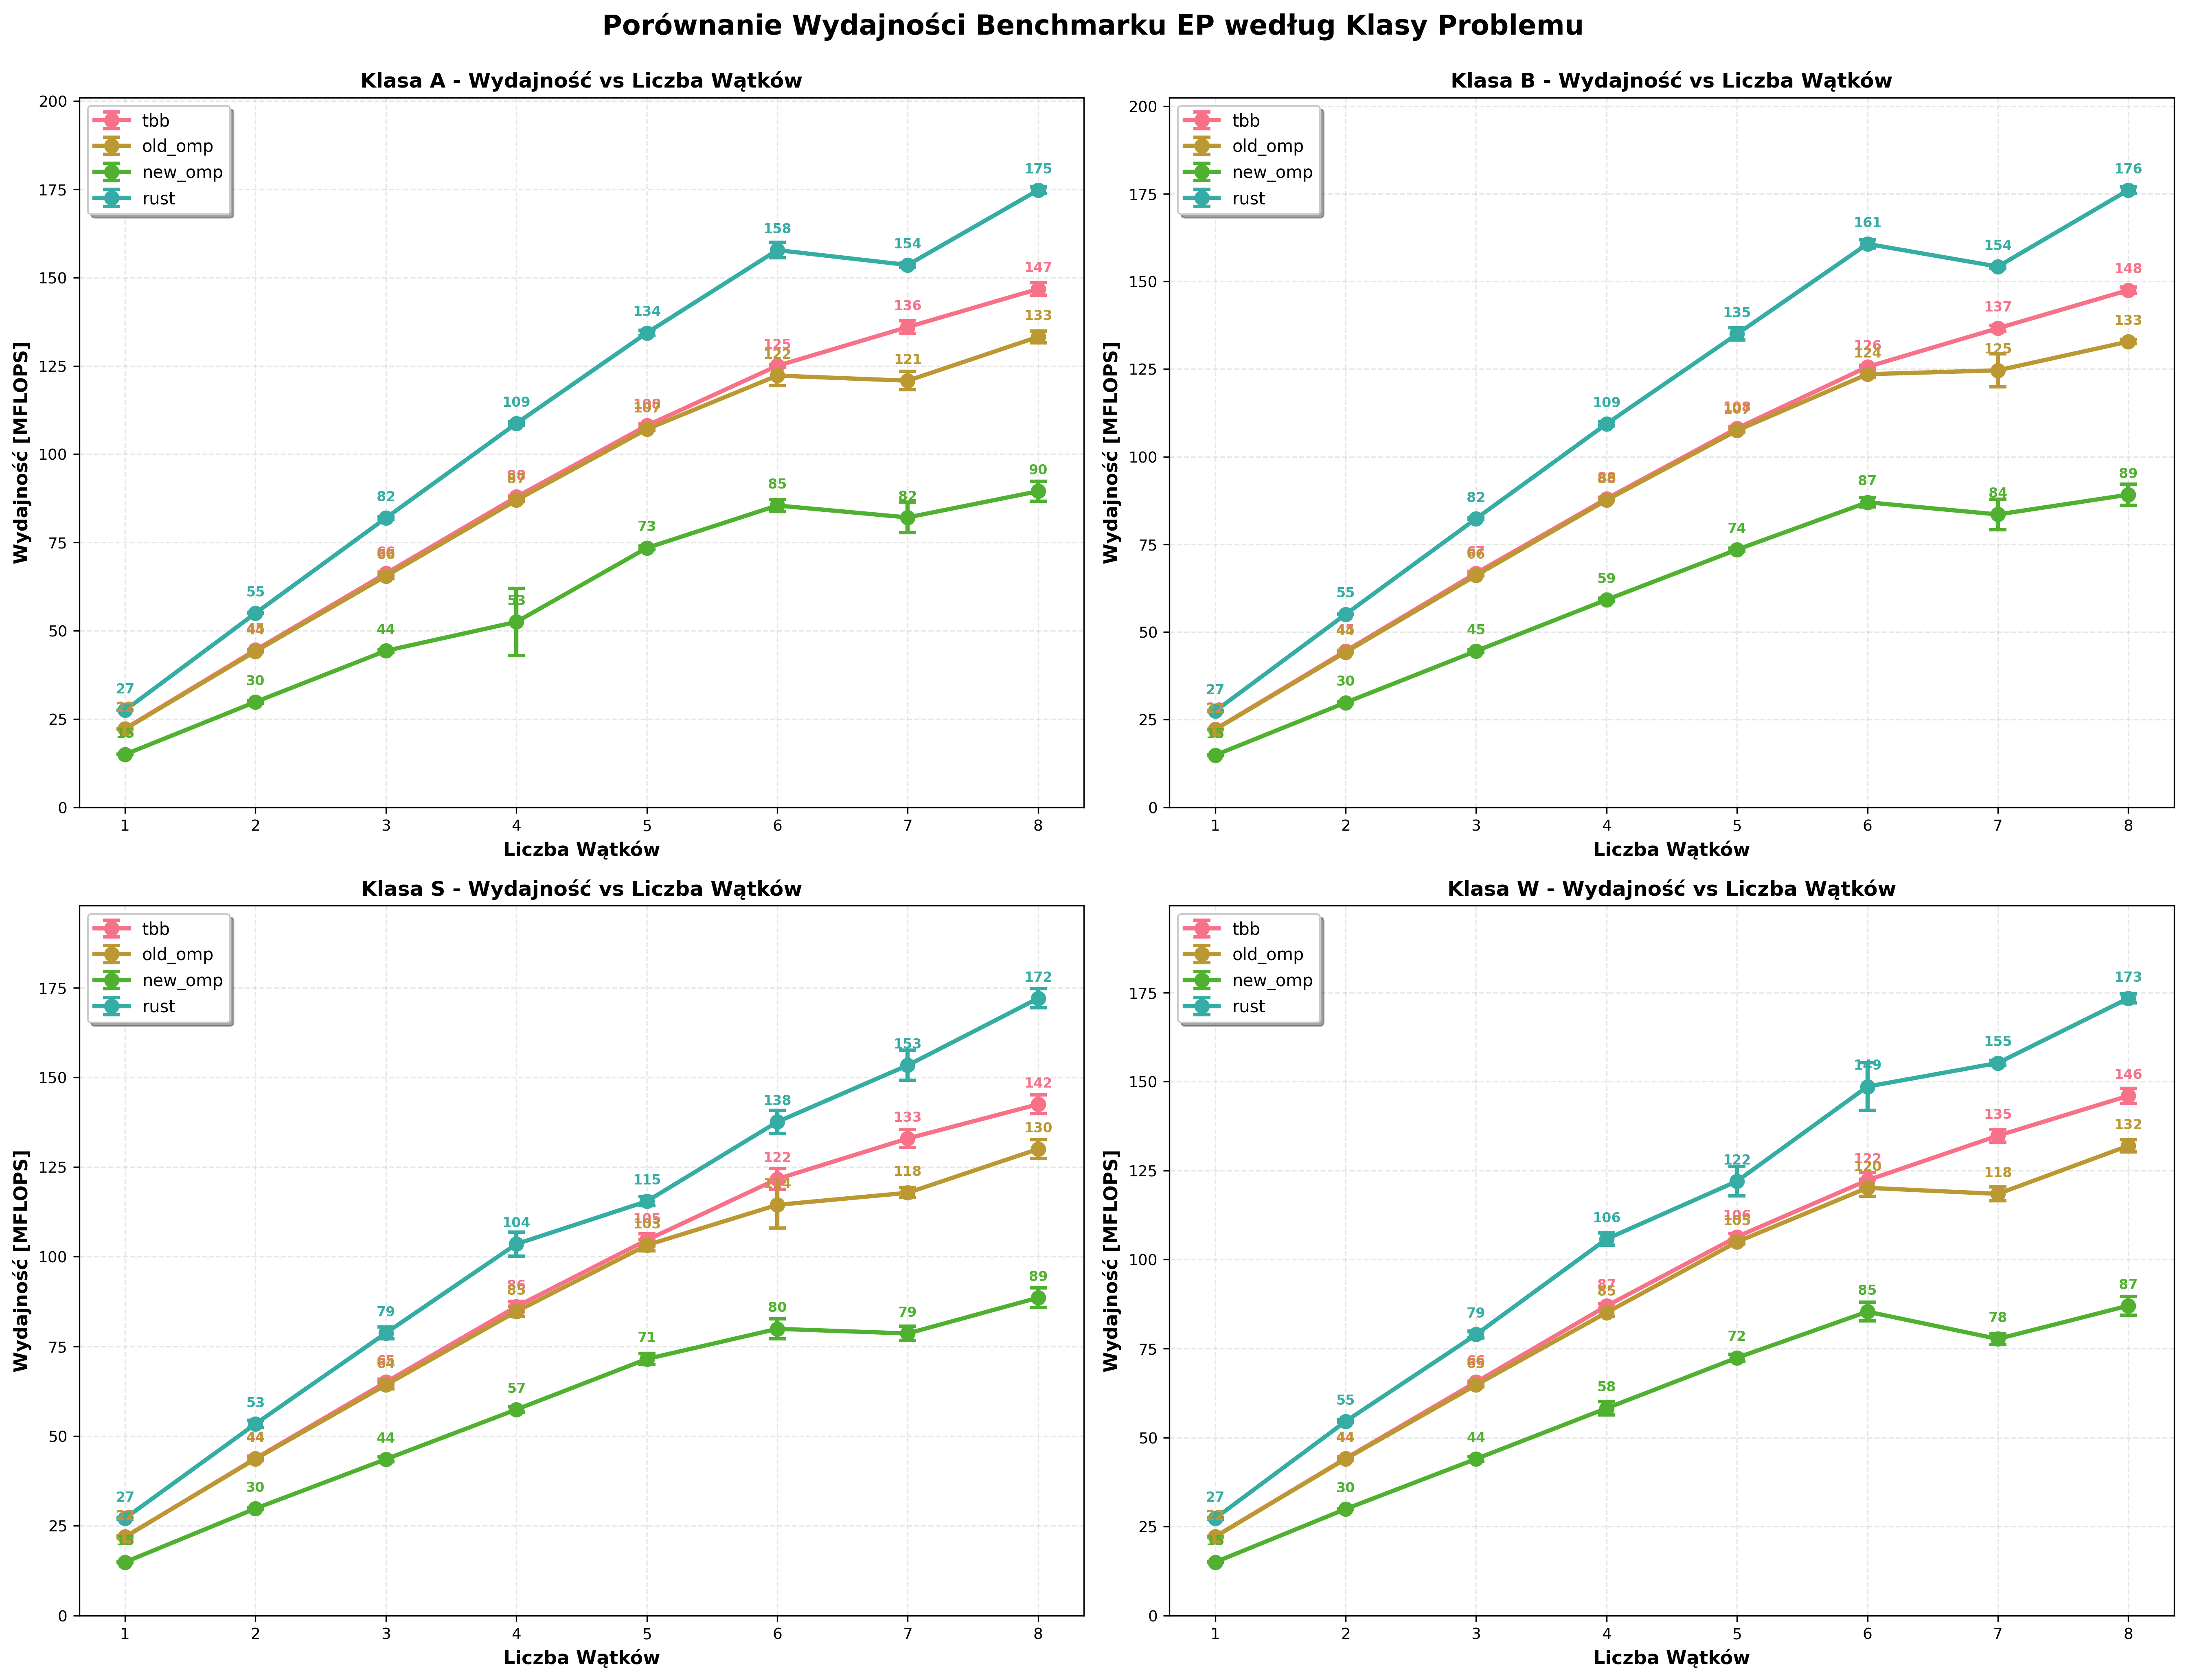
\includegraphics[width=0.9\textwidth]{analiza/images/parallel/ep/x86/ep_porownanie_wydajnosci.png}
    \caption{Porównanie wydajności benchmarku EP dla klas S, W, A, B względem liczby użytych wątków}
    \label{ep_porownanie_wydajnosci_x86_64}
\end{figure}
Na rysunku \ref{ep_porownanie_wydajnosci_x86_64} przedstawiono porównanie wydajności benchmarku EP w milionach operacji zmiennoprzecinkowych na sekundę (MFLOPS) dla różnych klas problemu i liczby wątków. Wartości zostały przedstawione w skali logarytmicznej, co pozwala lepiej zobrazować różnice między implementacjami.

\begin{figure}[H]
    \centering
    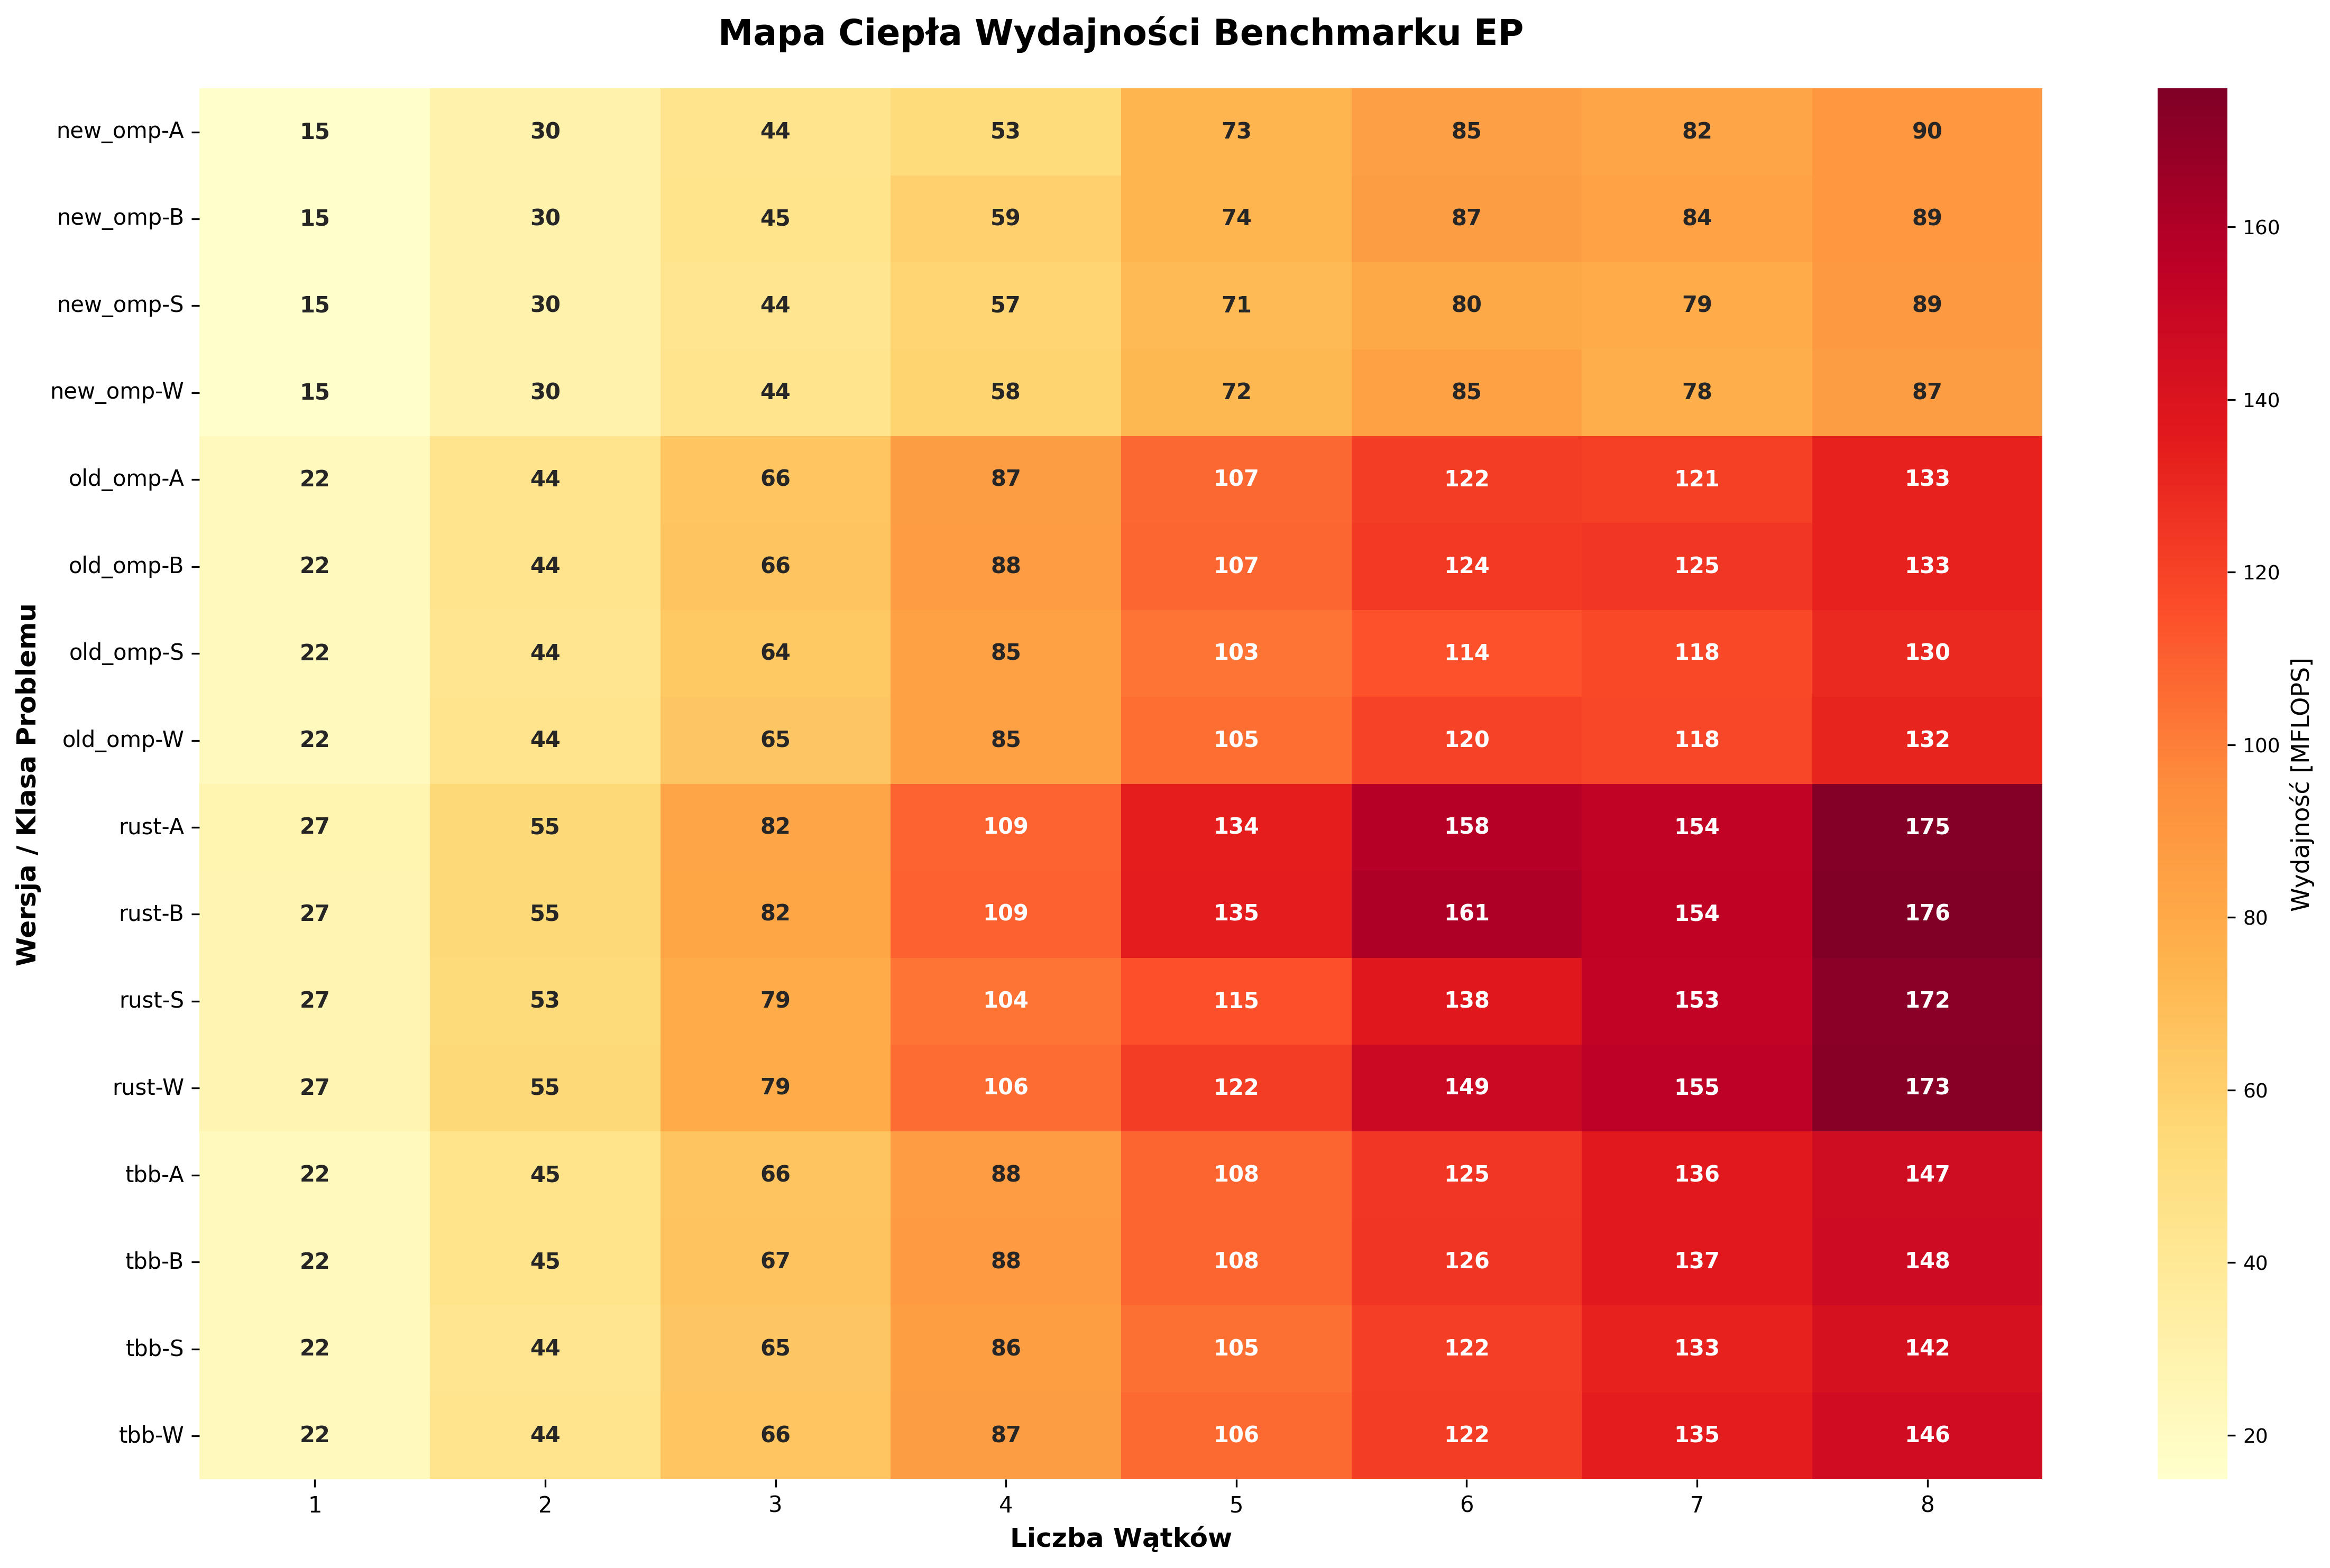
\includegraphics[width=0.9\textwidth]{analiza/images/parallel/ep/x86/ep_mapa_ciepla_wydajnosci.png}
    \caption{Mapa ciepła wydajności benchmarku EP dla klas S, W, A, B względem liczby użytych wątków}
    \label{ep_heatmap_wydajnosci_x86_64}
\end{figure}
Mapa ciepła - rysunek \ref{ep_heatmap_wydajnosci_x86_64} przedstawia wydajność benchmarku EP w zależności od liczby użytych wątków. Odcienie koloru od żółtego do ciemnoczerwonego wskazują na wzrost wydajności.\\


Wszystkie analizowane implementacje wykazują wzrost wydajności wraz ze zwiększaniem liczby wątków, co jest zgodne z oczekiwaniami dla algorytmów równoległych typu embarrassingly parallel. Najbardziej dynamiczny przyrost wydajności obserwowany jest w zakresie od \mbox{1 do 5} wątków. Po przekroczeniu tego progu krzywe wzrostu zaczynają się wyraźnie spłaszczać, co sugeruje osiągnięcie punktu nasycenia zasobów sprzętowych.

Spośród wszystkich rozwiązań, najwyższą wydajność osiąga implementacja napisana w języku Rust, konsekwentnie uzyskując największe wartości MFLOPS dla każdej z klas problemu. Przy 8 wątkach osiąga ona poziom około 172-176 MFLOPS, a jej przewaga staje się szczególnie widoczna przy wyższych stopniach równoległości.

Na drugim miejscu pod względem wydajności plasuje się implementacja TBB, osiągająca przy 8 wątkach wartości w przedziale około 142-148 MFLOPS. Niewiele niższe wyniki uzyskuje \texttt{old\_omp}, którego maksymalna wydajność w tej konfiguracji wynosi około 130-133 MFLOPS.

Najniższe rezultaty pod względem MFLOPS odnotowano dla implementacji \texttt{new\_omp}, która przy 8 wątkach osiąga maksymalnie około 87-90 MFLOPS.

Dodatkowo, we wszystkich implementacjach zaobserwowano niewielkie wahania wydajności pomiędzy 6 a 7 wątkami. Może to wskazywać na wpływ czynników zależnych od architektury sprzętowej lub mechanizmów zarządzania zasobami stosowanych przez system operacyjny.

\begin{figure}[H]
    \centering
    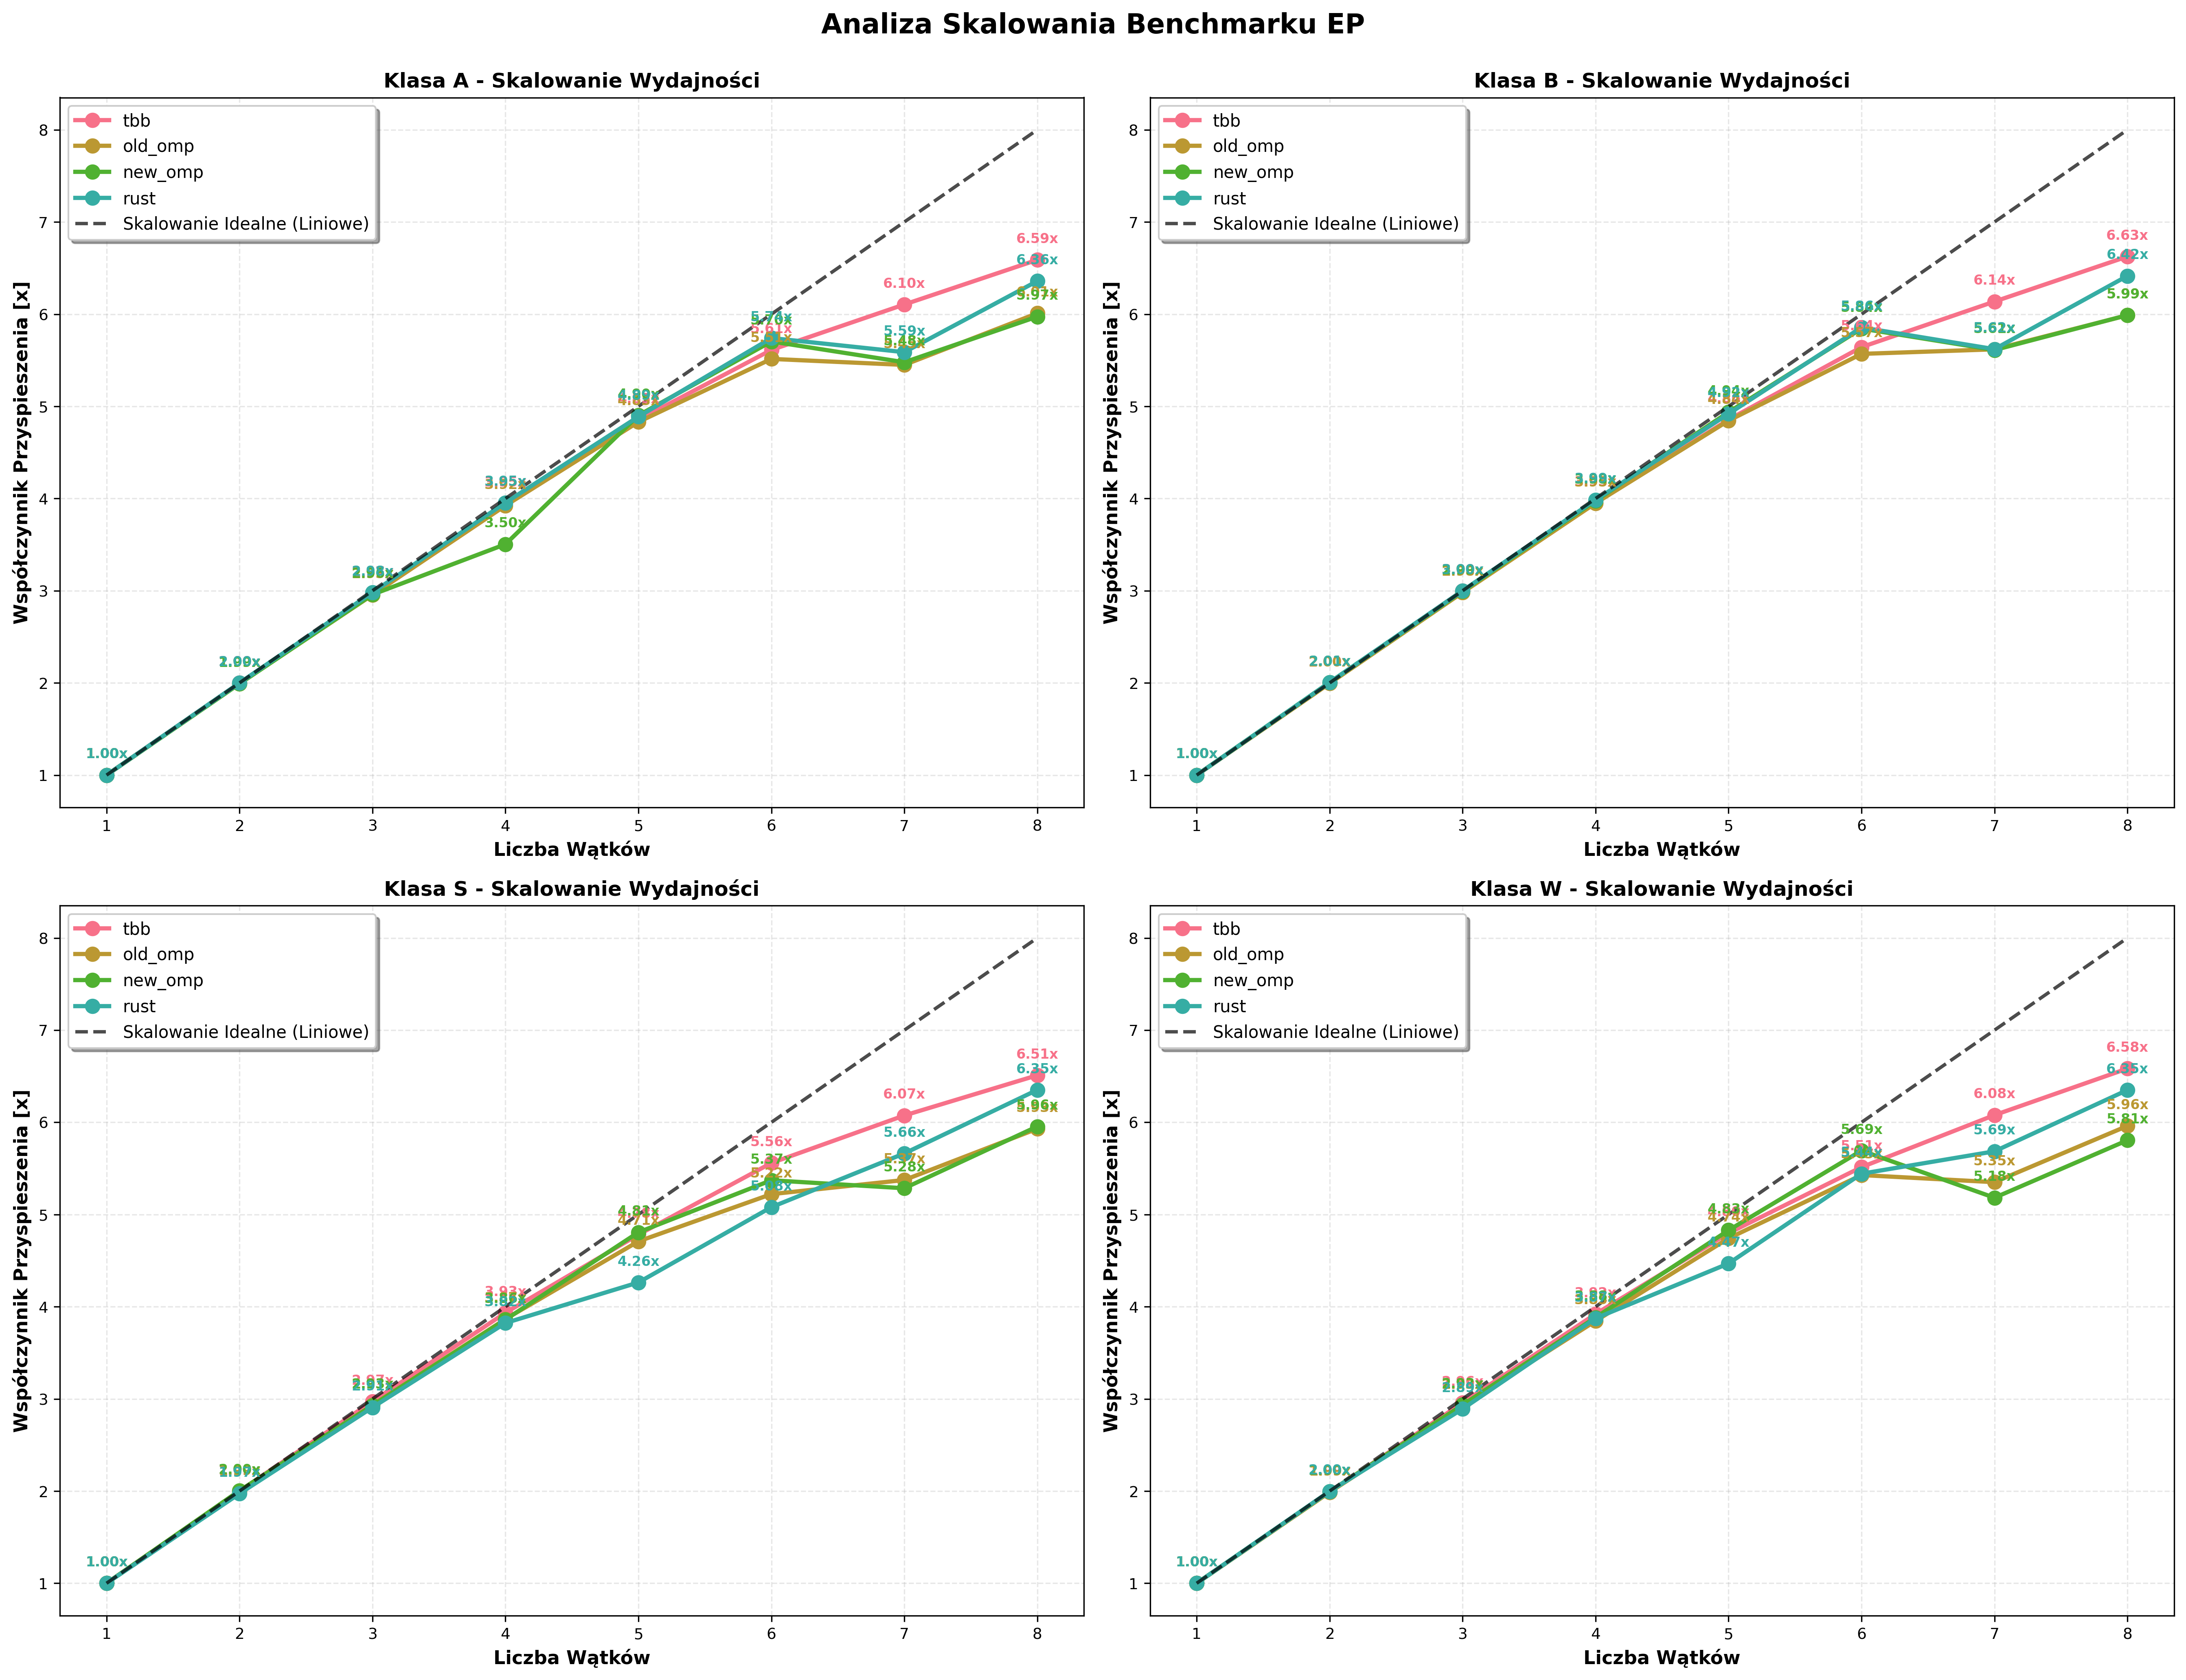
\includegraphics[width=0.9\textwidth]{analiza/images/parallel/ep/x86/ep_analiza_skalowania.png}
    \caption{Analiza skalowania benchmarku EP dla klas S, W, A, B względem liczby użytych wątków}
    \label{ep_analiza_skalowania_x86_64}
\end{figure}
Wykres - rysunek \ref{ep_analiza_skalowania_x86_64} przedstawia analizę skalowania wydajności benchmarku EP w zależności od liczby użytych wątków. Skalowanie zostało wyrażone jako współczynnik przyspieszenia względem wykonania jednowątkowego i odniesione do idealnego skalowania liniowego.

\subsubsection{Analiza wspólnych wzorców skalowania}
Analiza wykresów przedstawiających współczynniki przyspieszenia pozwala zidentyfikować kilka istotnych wzorców. We wszystkich implementacjach zaobserwowano niemal liniowe skalowanie w zakresie od 1 do 4 wątków. Współczynniki przyspieszenia w tym przedziale są zbliżone do wartości idealnej, co świadczy o wysokiej efektywności równoległej algorytmu EP w warunkach ograniczonego współdzielenia zasobów.

Po przekroczeniu czterech wątków, a więc w zakresie od 5 do 8, wszystkie implementacje zaczynają wykazywać stopniowe odchylenia od skalowania idealnego. Zjawisko to jest typowe dla obliczeń równoległych i wynika z narzutów komunikacyjnych, współdzielenia zasobów sprzętowych, a także ograniczeń wynikających z architektury systemu oraz kosztów synchronizacji.

Ciekawym elementem analizy jest występowanie lokalnego maksimum współczynnika przyspieszenia przy sześciu wątkach, po którym przy siedmiu wątkach następuje niewielki spadek. Może to wskazywać na wpływ specyfiki architektury procesora lub strategii planowania zadań stosowanych przez system operacyjny.

Przy maksymalnej liczbie ośmiu wątków ponownie obserwuje się wzrost współczynnika przyspieszenia we wszystkich implementacjach, co sugeruje efektywniejsze wykorzystanie zasobów obliczeniowych w sytuacji pełnego obciążenia systemu.

\subsubsection{Porównanie efektywności różnych implementacji}
Spośród wszystkich badanych rozwiązań, implementacja w języku Rust osiąga najwyższe współczynniki przyspieszenia przy ośmiu wątkach, z wartościami rzędu 6,4-6,5x względem wersji jednowątkowej. Wskazuje to na wysoką efektywność tej implementacji pod względem skalowania równoległego.

Intel TBB uzyskuje nieznacznie niższe, lecz wciąż bardzo dobre wyniki skalowania, osiągając przyspieszenie na poziomie 6,1-6,3x przy ośmiu wątkach. Obie wersje OpenMP, tj. \texttt{old\_omp} i~\texttt{new\_omp}, osiągają nieco niższe współczynniki przyspieszenia, mieszczące się w przedziale 5,8-6,1x, co czyni je mniej efektywnymi w porównaniu z implementacją w języku Rust oraz TBB.

Warto również zaznaczyć, że w przedziale 4-6 wątków wszystkie implementacje osiągają bardzo zbliżone wyniki, co wskazuje na podobną efektywność w wykorzystaniu średniego poziomu równoległości oraz dostępnych rdzeni obliczeniowych.

\subsection{Wyniki profilowania wydajności - platforma ARM64}
W celu kompleksowego porównania efektywności testowanych implementacji benchmarku EP na platformie ARM64 dokonano analizy metryk systemowych dotyczących zarządzania pamięcią: zużycia pamięci \eng{memory usage}, liczby odzyskanych stron pamięci \eng{page reclaims}, liczby błędów stron pamięci \eng{page faults} oraz ich wzajemnych relacji.
\begin{figure}[H]
    \centering
    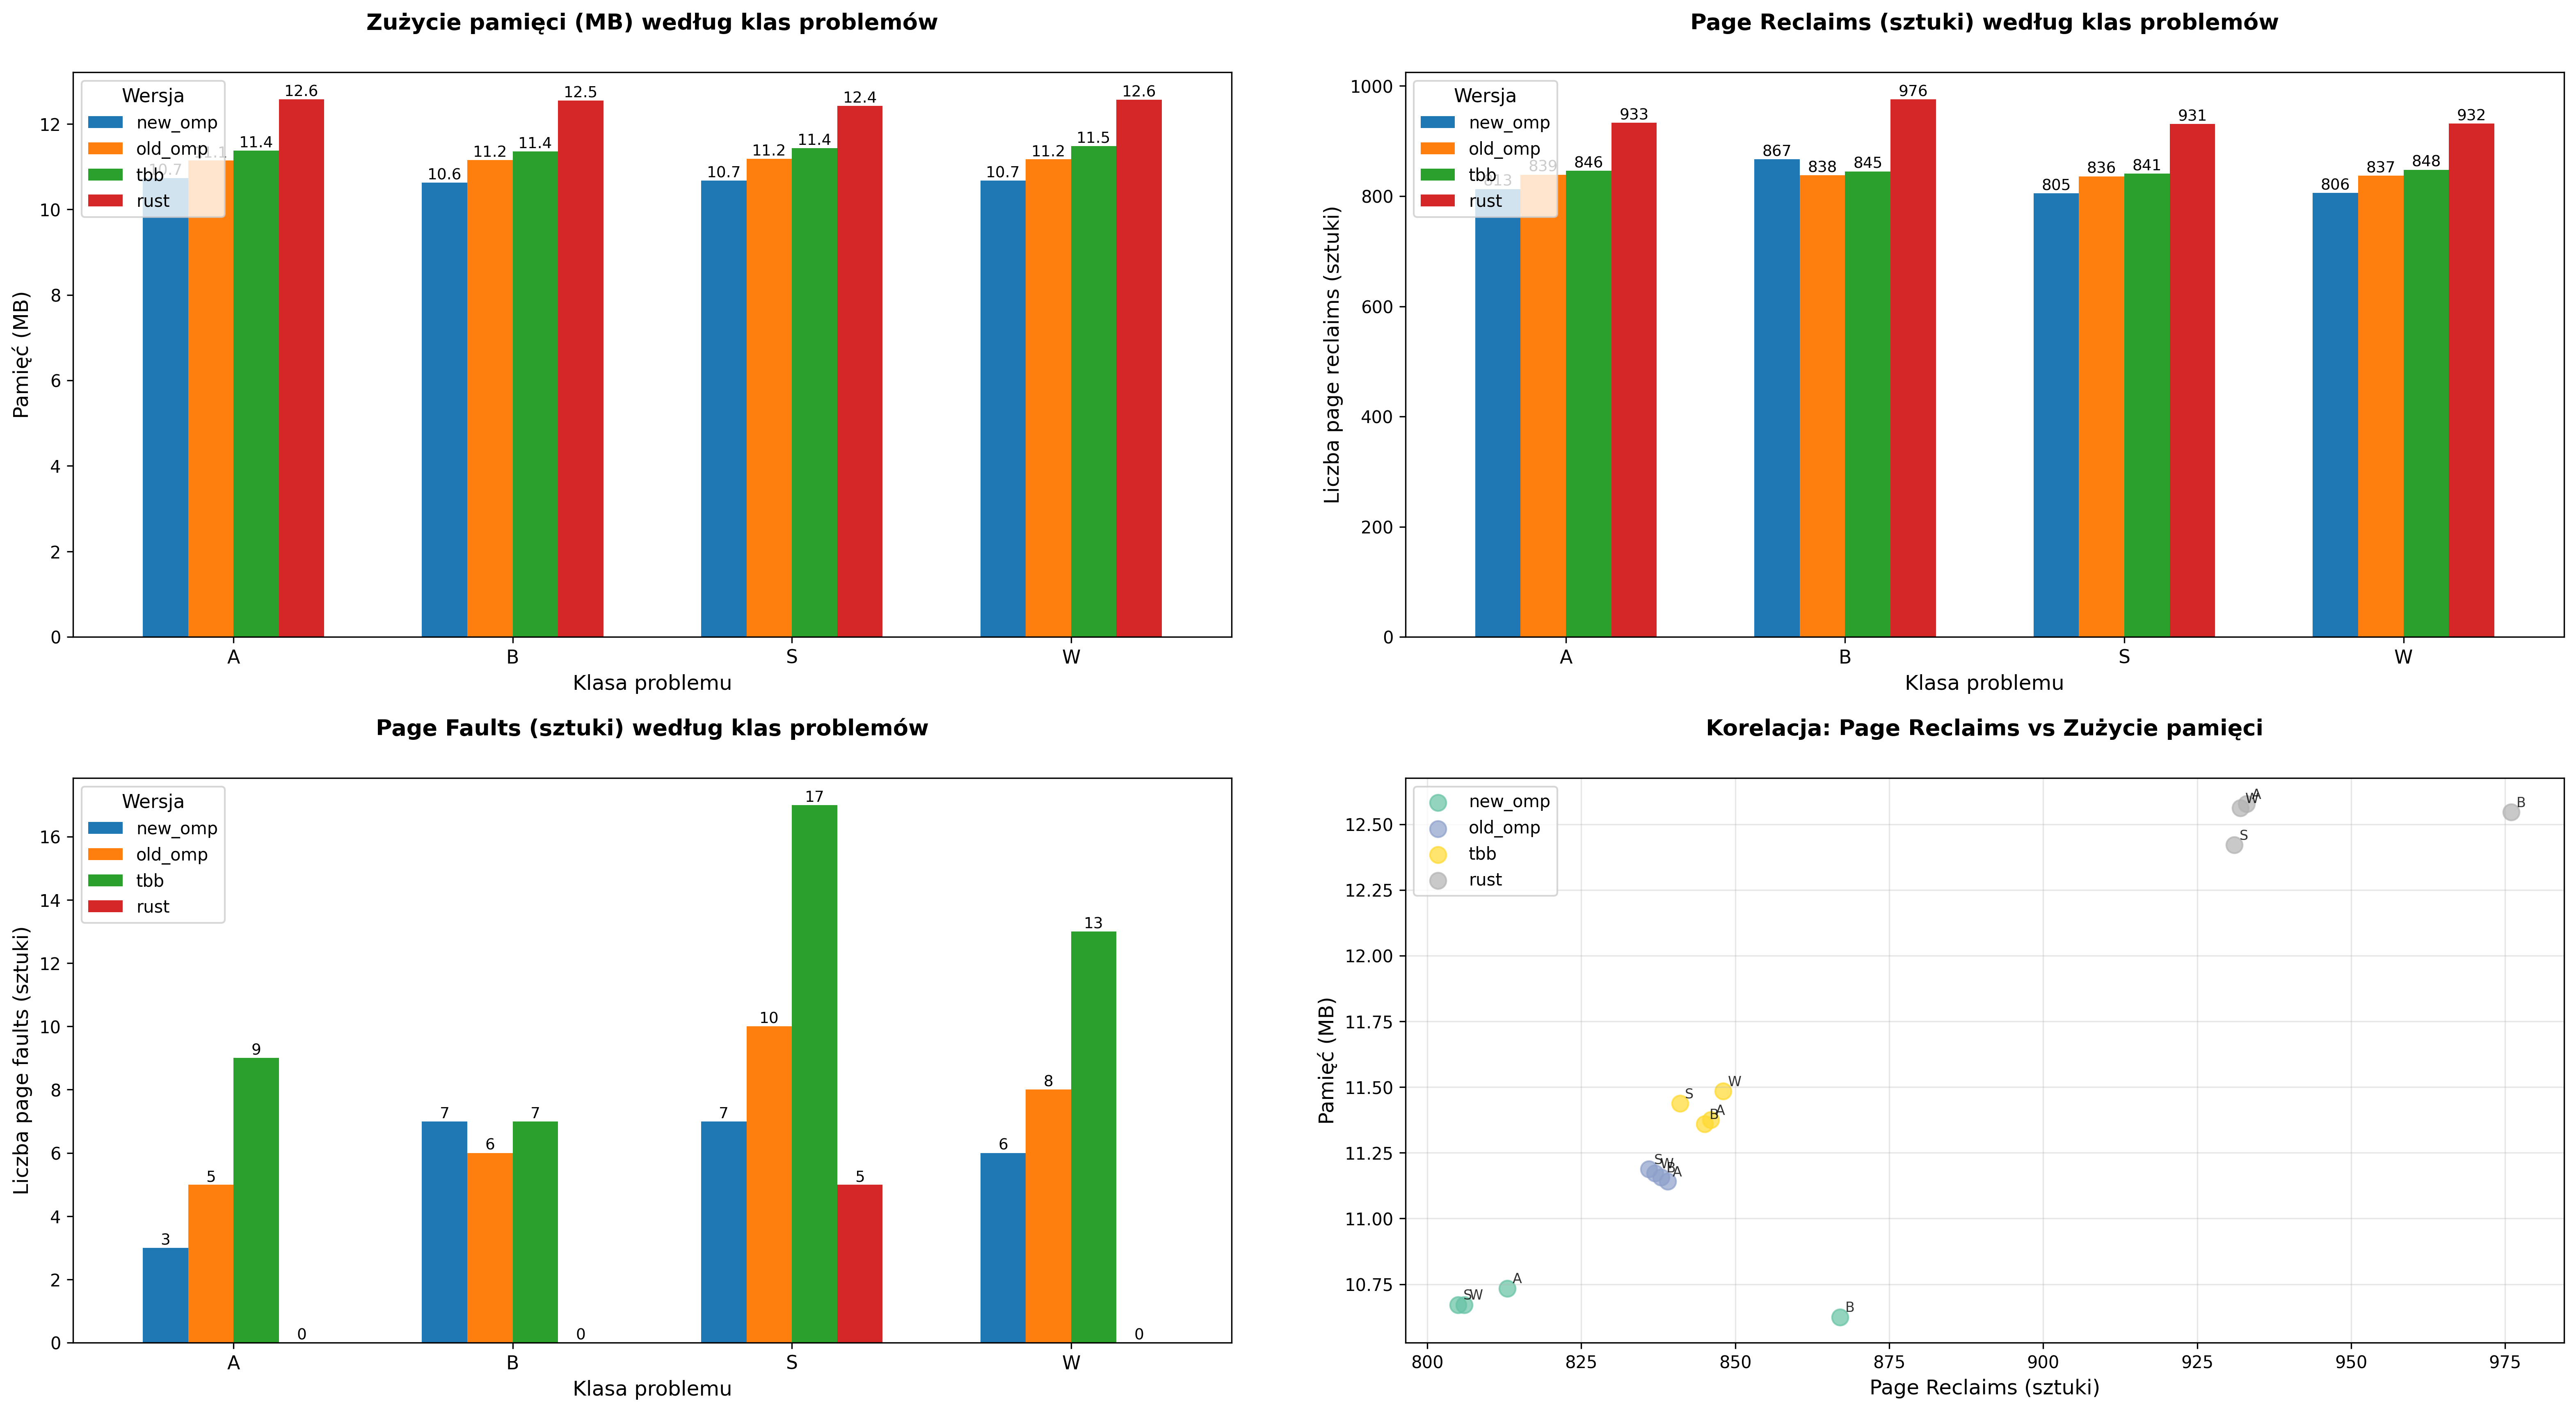
\includegraphics[width=0.9\textwidth]{analiza/images/parallel/ep/arm/chart_01_memory_comparison.png}
    \caption{Profilowanie wydajności benchmarku EP dla klas S, W, A, B względem liczby użytych wątków}
    \label{ep_porownanie_zuzycia_pamieci}
\end{figure}
 


\begin{figure}[H]
    \centering
    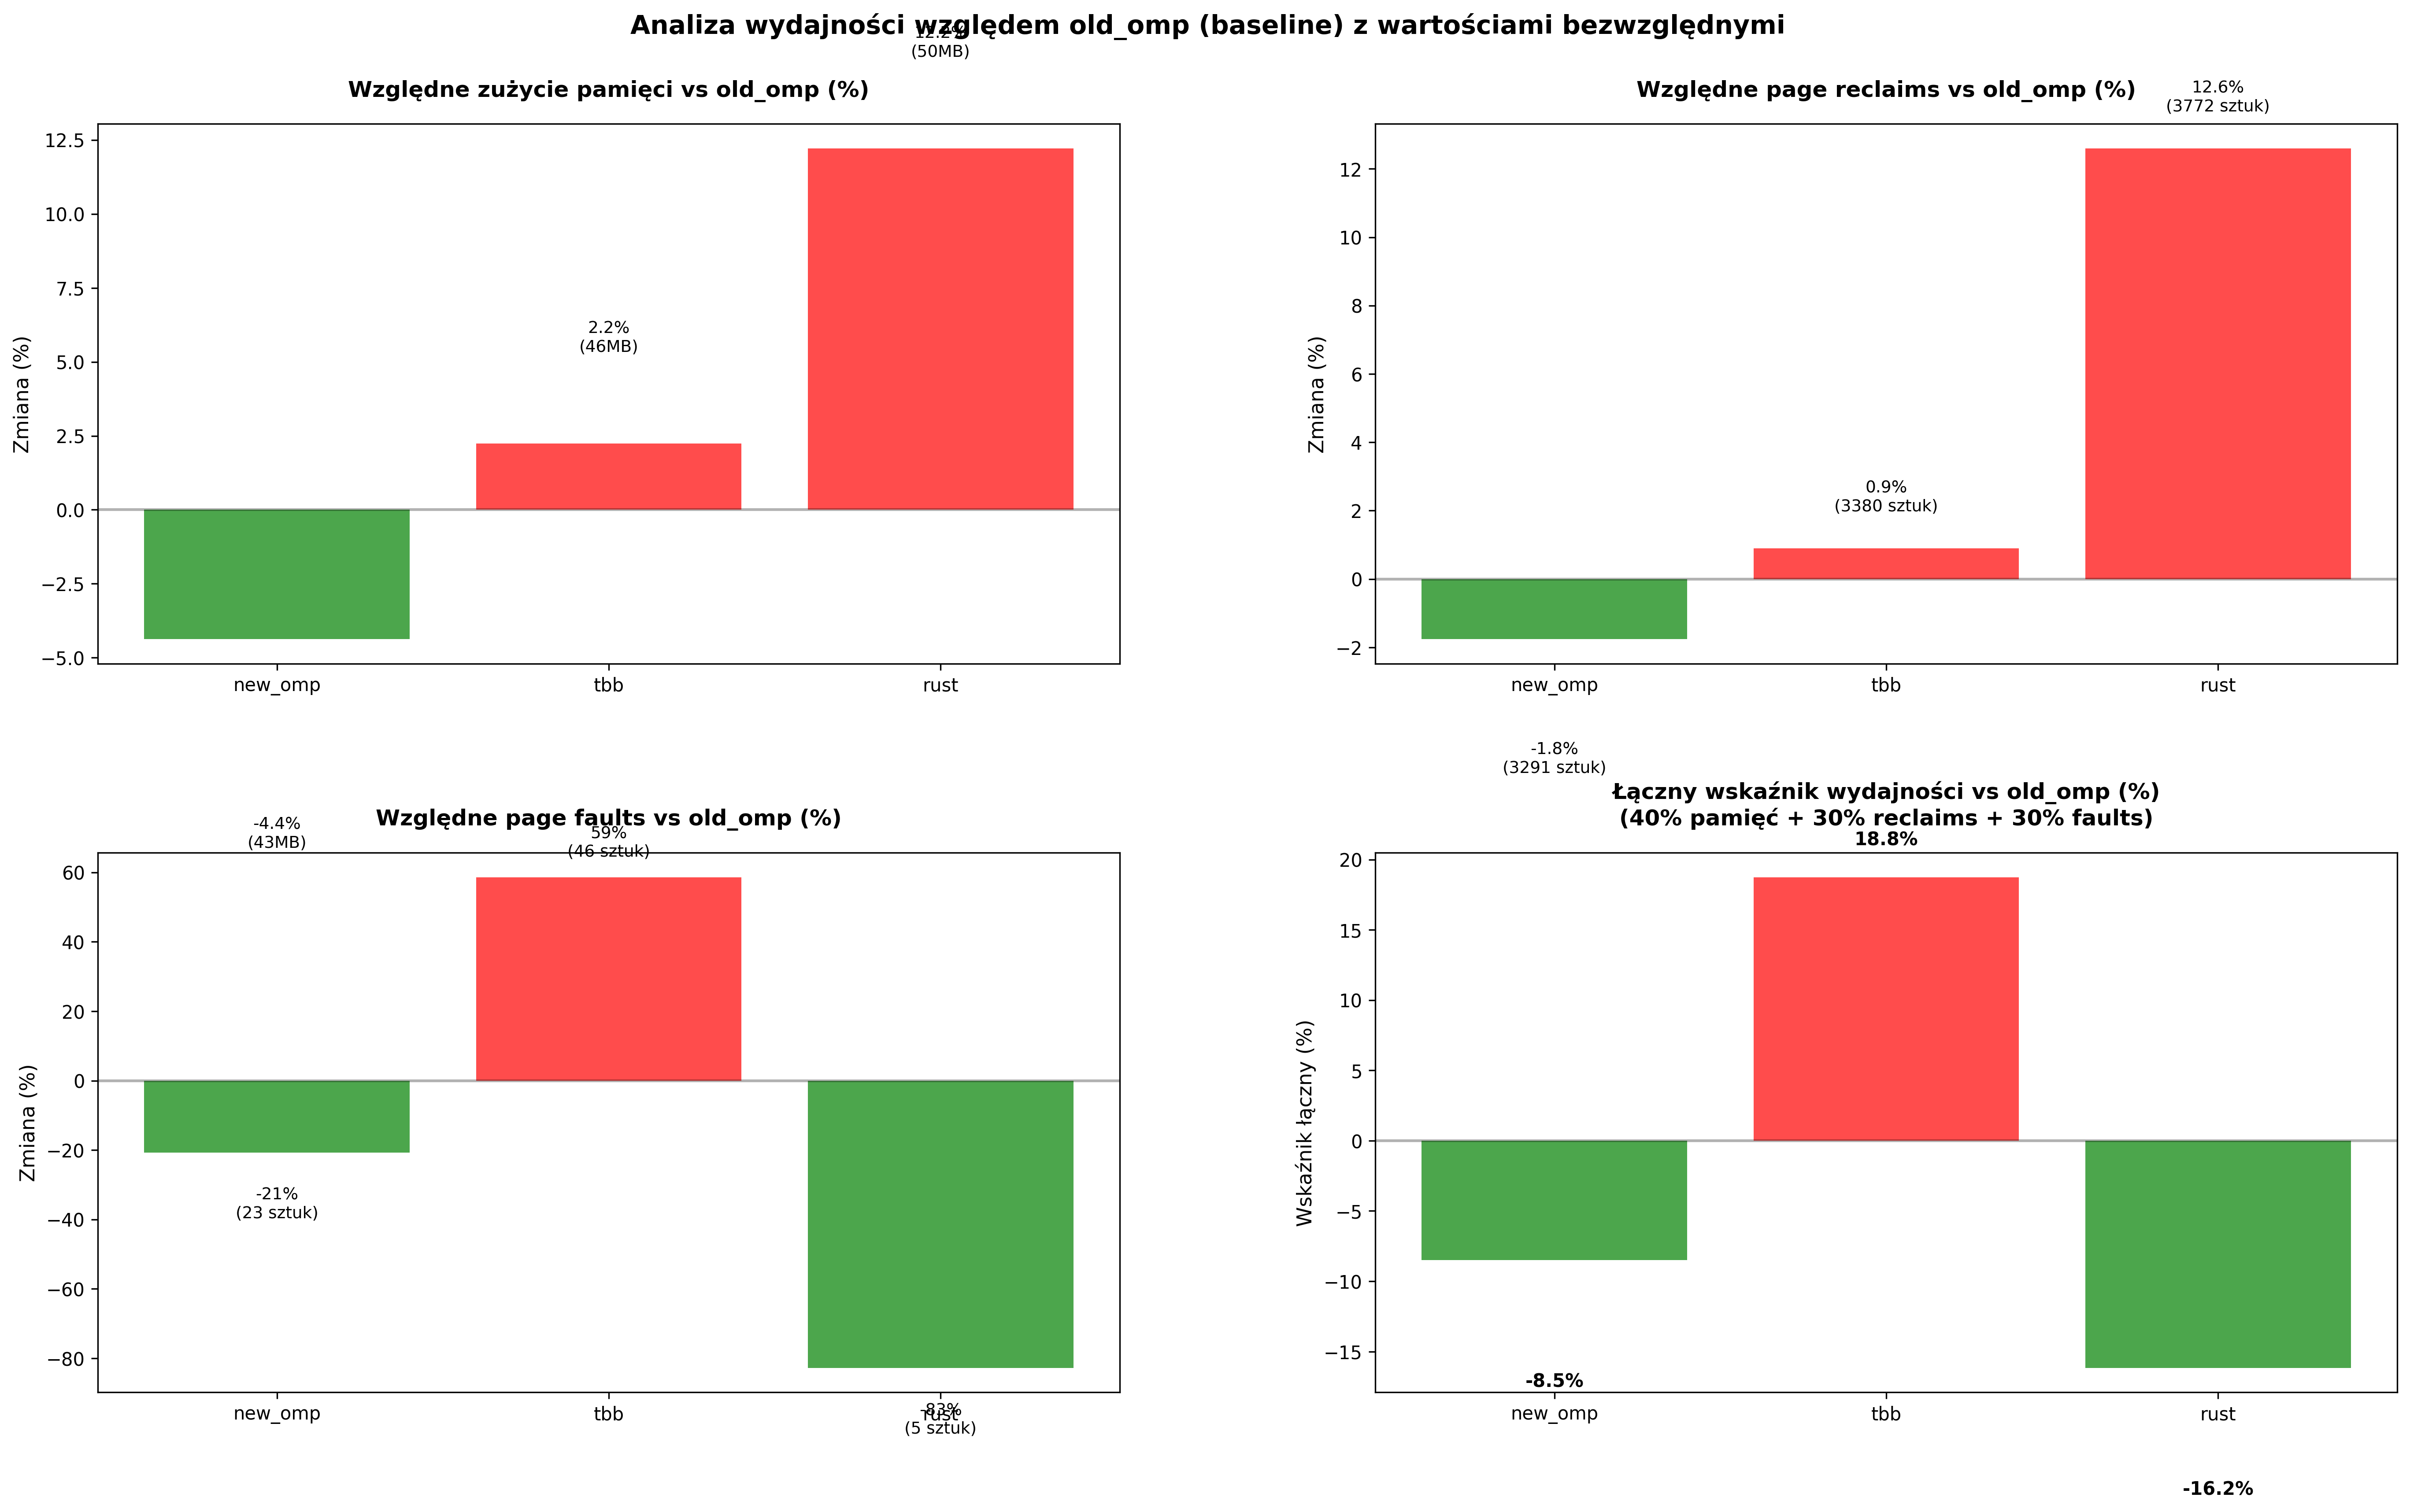
\includegraphics[width=0.9\textwidth]{analiza/images/parallel/ep/arm/chart_05_performance_ratios.png}
    \caption{Analiza wydajności względem \texttt{old\_omp} (punkt odniesienia) z wartościami bezwzględnymi}
    \label{ep_analiza_wzgledem_old_omp}
\end{figure}
Na rysunku \ref{ep_analiza_wzgledem_old_omp} zestawiono zmiany procentowe trzech analizowanych wskaźników względem implementacji referencyjnej \texttt{old\_omp}. Wskaźnikiem syntetycznym jest łączna metryka złożona z ważonych proporcji zużycia pamięci (40\%), zwolnionych stron (30\%) i błędów stron (30\%).



\begin{figure}[H]
    \centering
    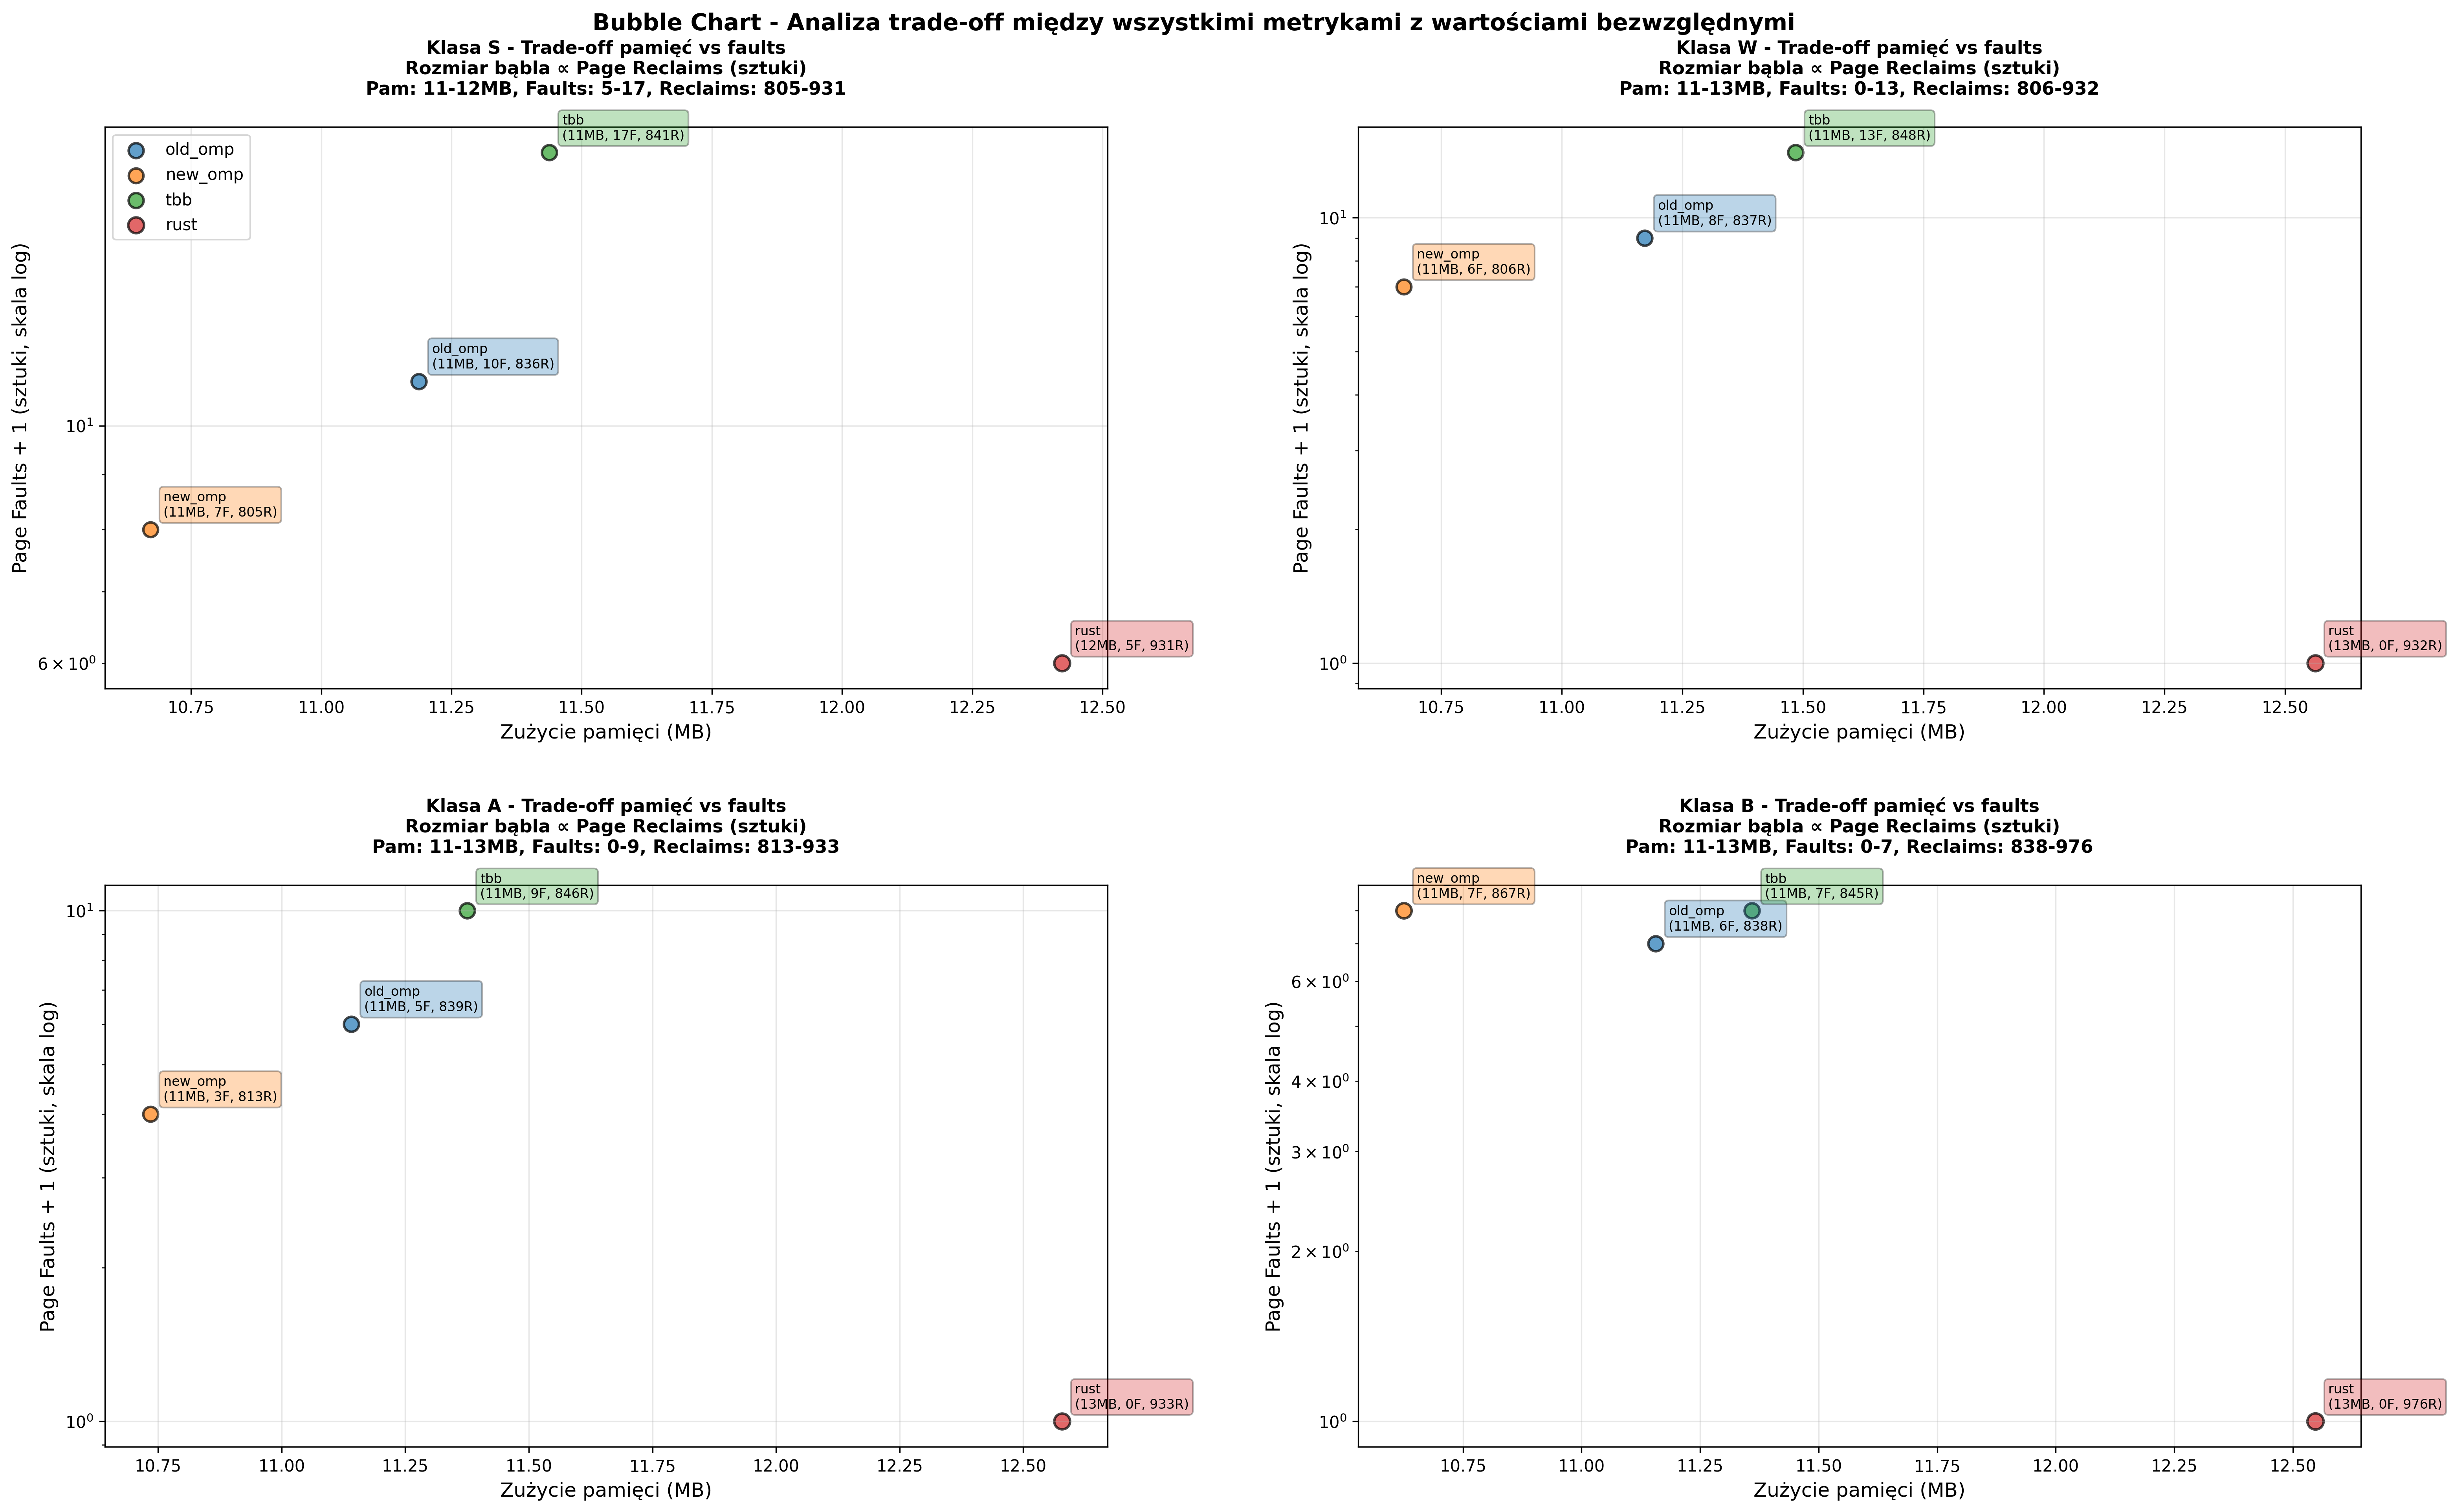
\includegraphics[width=0.9\textwidth]{analiza/images/parallel/ep/arm/chart_06_bubble_chart.png}
    \caption{Kompromisy \eng{trade-off} pomiędzy zużyciem pamięci a błędami stron pamięci, z uwzględnieniem liczby odzyskanych stron jako trzeciej zmiennej reprezentowanej przez rozmiar bąbla}
    \label{ep_kompromisy_pamiec_bledy}
\end{figure}
Rysunek \ref{ep_kompromisy_pamiec_bledy} przedstawia kompromisy\eng{trade-offs} między zużyciem pamięci a błędami stron, z liczbą odzyskanych stron jako trzecim wymiarem (rozmiar bąbla). Oś Y jest przedstawiona w skali logarytmicznej ze względu na zróżnicowaną skalę błędów stron.


\subsection{Wyniki profilowania wydajności - platforma x86\_64}
\begin{figure}[H]
    \centering
    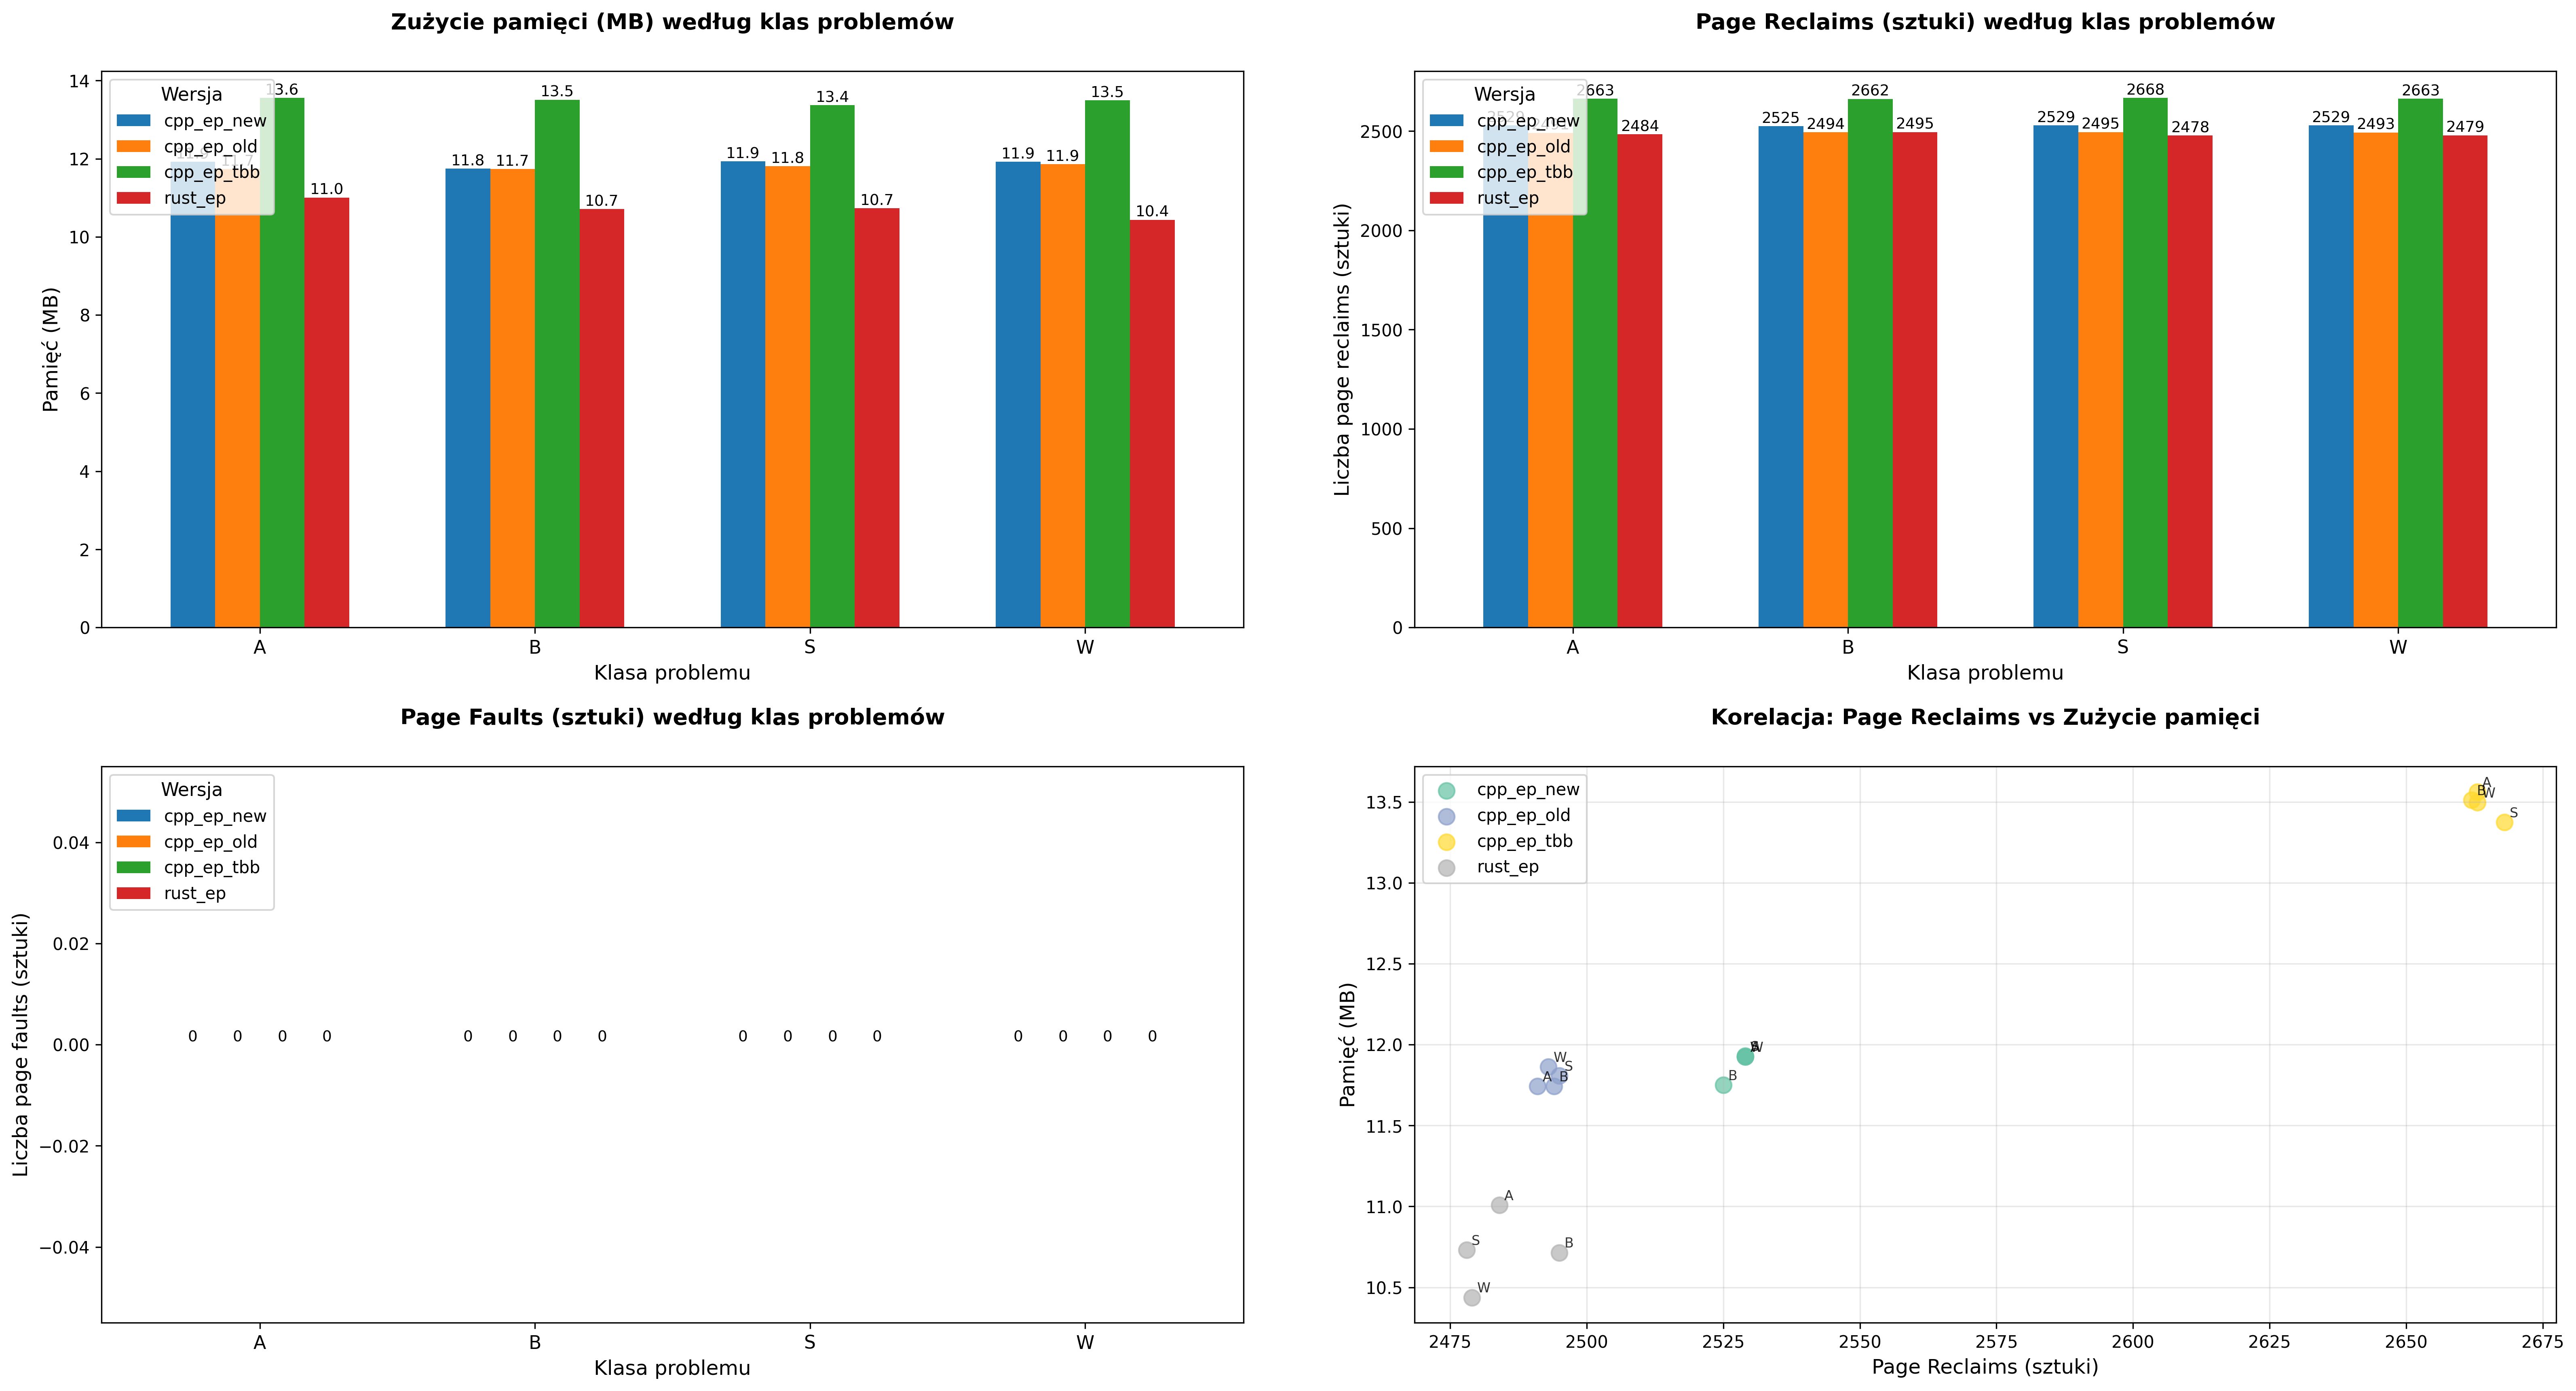
\includegraphics[width=0.9\textwidth]{analiza/images/parallel/ep/x86/chart_01_memory_comparison.png}
    \caption{Profilowanie wydajności benchmarku EP dla klas S, W, A, B względem liczby użytych wątków}
    \label{ep_porownanie_zuzycia_pamieci_x86_64}
\end{figure}
\begin{figure}[H]
    \centering
    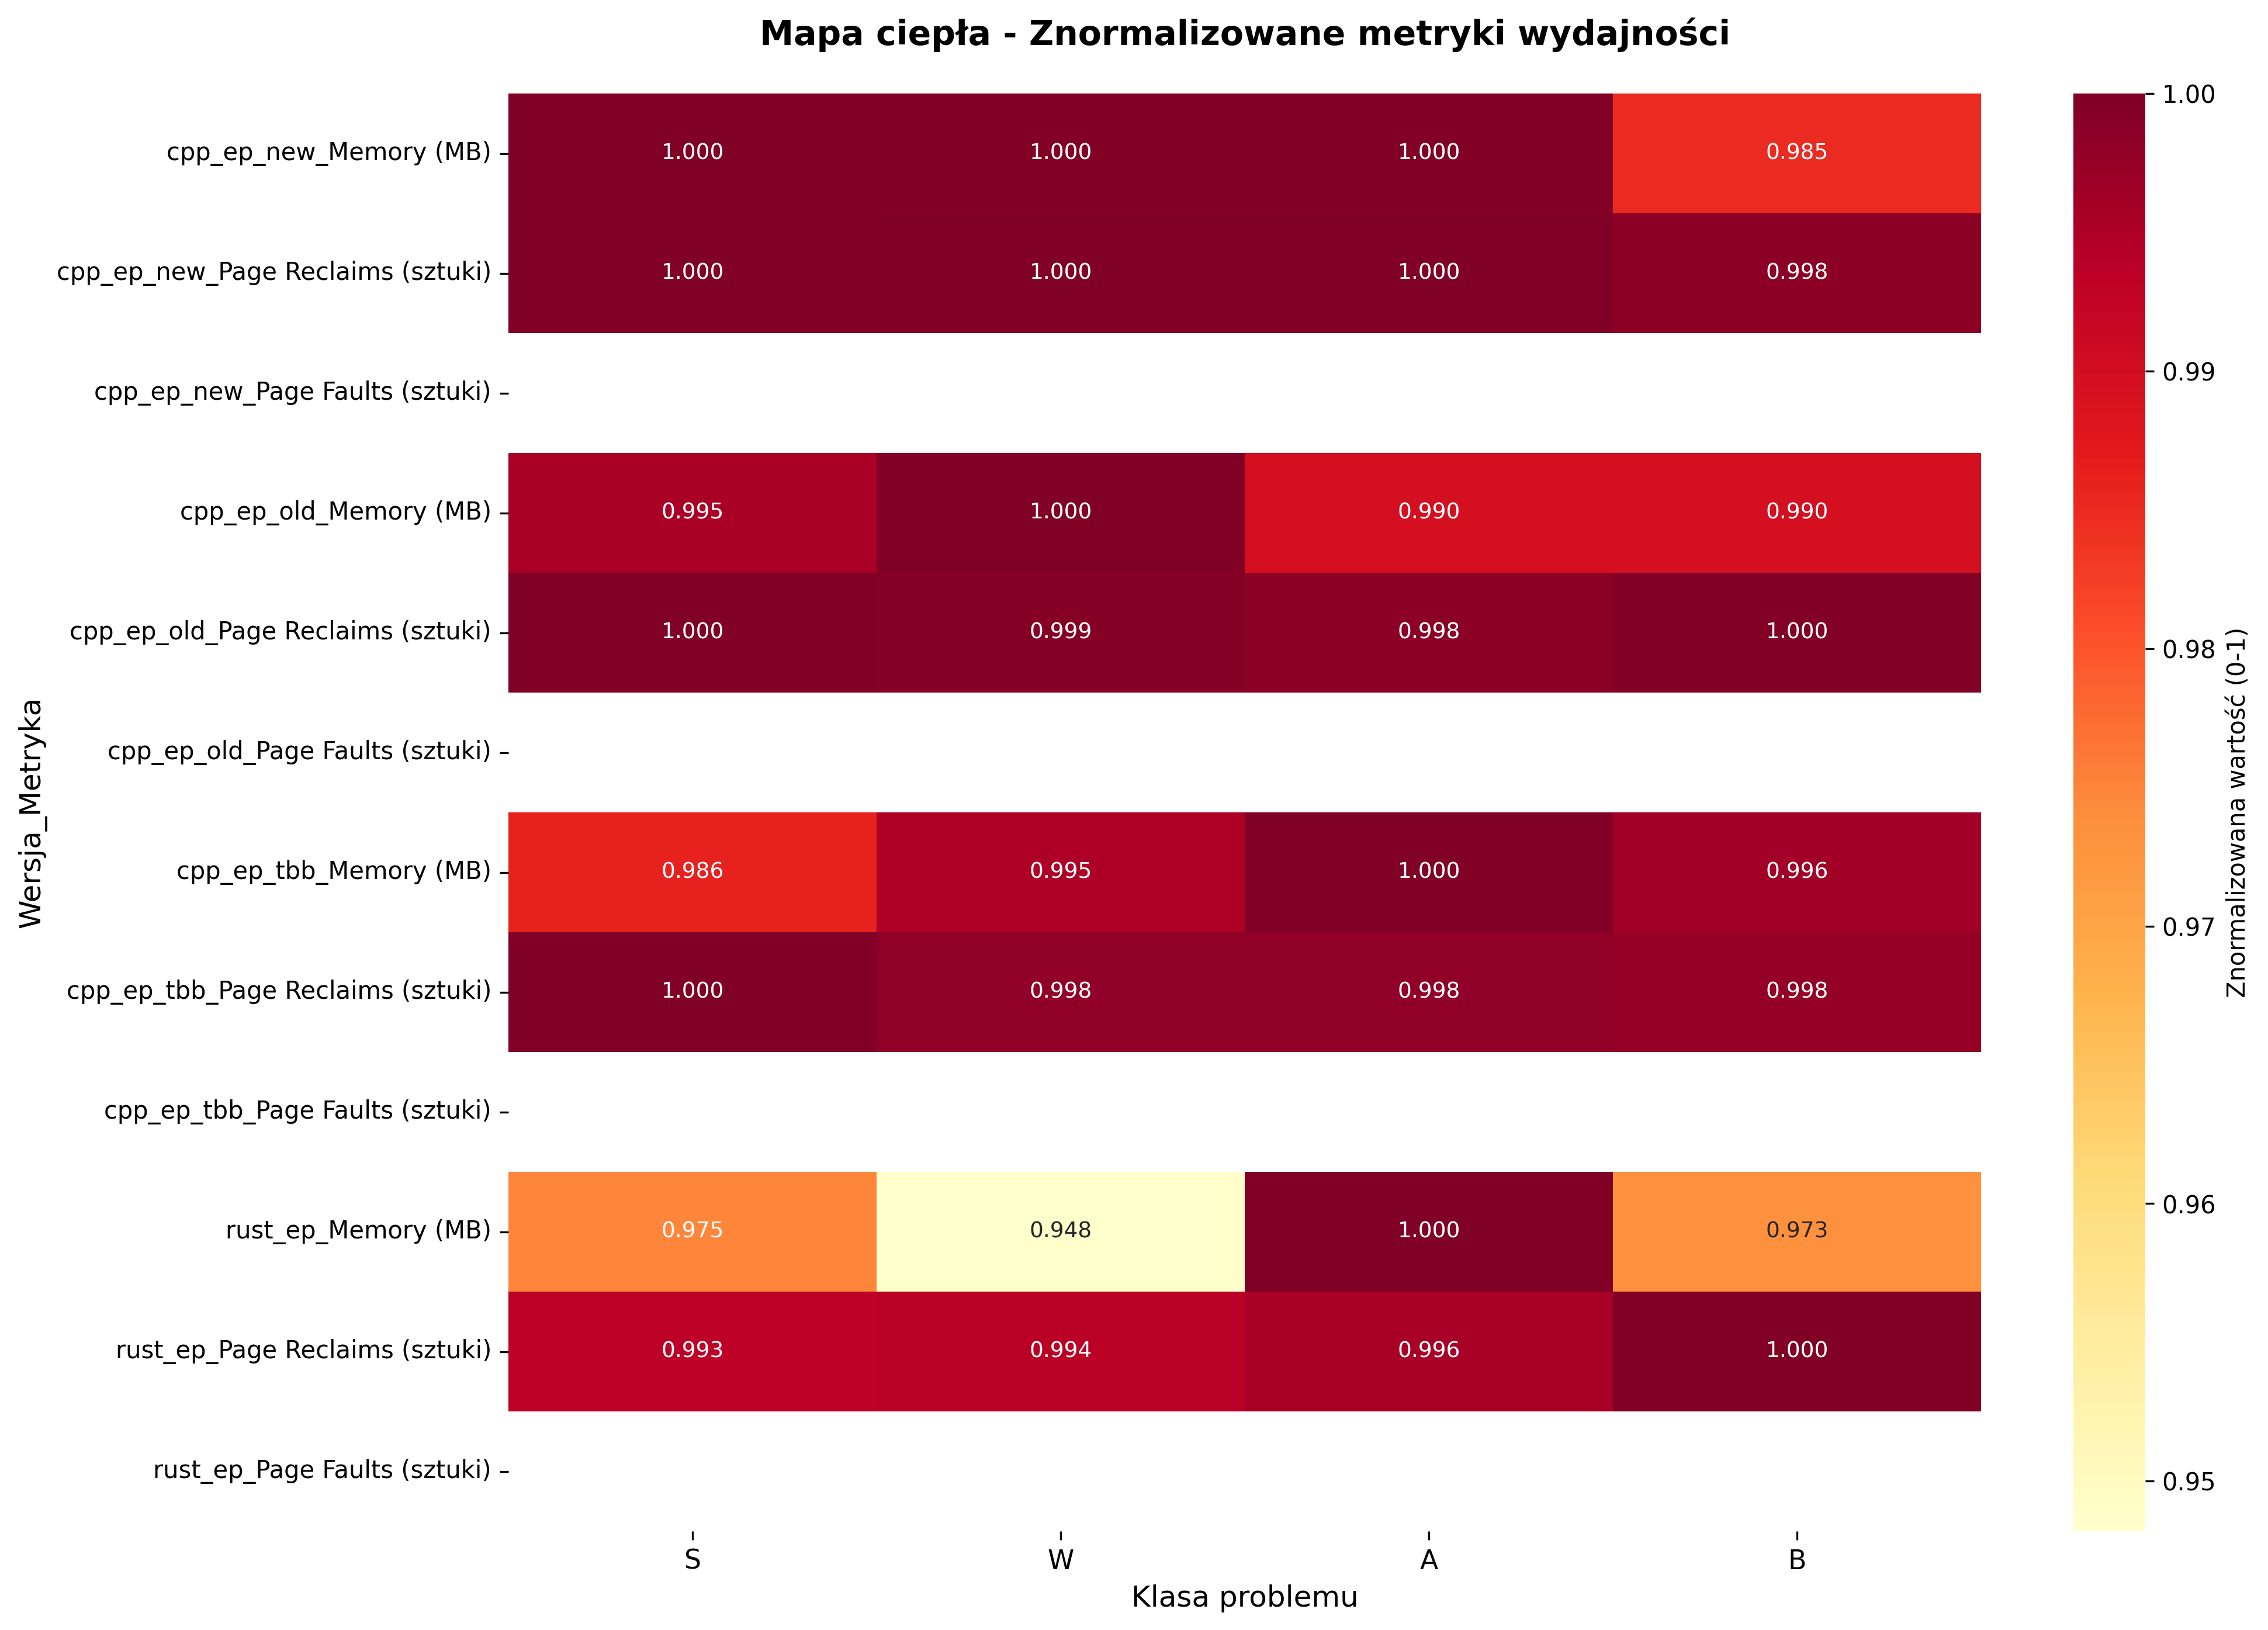
\includegraphics[width=0.9\textwidth]{analiza/images/parallel/ep/x86/chart_03_heatmap.png}
    \caption{Znormalizowana mapa metryk pamięciowych}
    \label{ep_znormalizowana_mapa_metryk}
\end{figure}
\subsubsection{Analiza zużycia i zarządzania pamięcią}
W analizie zużycia pamięci zauważalne są istotne różnice pomiędzy implementacjami. Największe zużycie pamięci systemowej wykazuje implementacja \texttt{new\_omp}, osiągając w każdej klasie problemu wartość rzędu 13,4-13,6 MB. Szczególnie stabilny poziom zużycia tej implementacji widoczny jest w klasach B, S i W, gdzie wartość oscyluje wokół 13,5 MB.

Zupełnie odmienną charakterystyką wyróżnia się implementacja \texttt{rust}, która wykazuje najniższe zużycie pamięci w przedziale 10,4-11,0 MB. Oznacza to około 22\% oszczędności względem najbardziej pamięciochłonnej wersji, co świadczy o lepszym zarządzaniu alokacją zasobów. Pozostałe dwie implementacje, \texttt{old\_omp} i \texttt{tbb}, prezentują bardzo zbliżone wartości zużycia pamięci, mieszczące się w zakresie 11,8-11,9 MB, co pozycjonuje je pośrednio pomiędzy skrajnymi przypadkami.

Co istotne, zużycie pamięci dla każdej implementacji pozostaje stosunkowo stałe w obrębie różnych klas problemu. Sugeruje to, że wielkość instancji problemu EP nie wpływa istotnie na alokację pamięci, a struktury danych i strategie zarządzania pamięcią są zaprojektowane w~sposób odporny na zmiany skali.

\subsubsection{Operacje pamięci wirtualnej}
Analiza operacji związanych z pamięcią wirtualną - w szczególności liczby odzyskanych stron oraz liczby błędów strony - dostarcza dodatkowych informacji o efektywności systemu operacyjnego i implementacji.

Wszystkie implementacje odnotowują zbliżoną liczbę odzyskanych stron, w zakresie od 2475 do 2665. Najwyższy poziom zwolnień stron występuje w implementacji \texttt{tbb} dla klasy W (2663), podczas gdy \texttt{rust} konsekwentnie utrzymuje nieco niższe wartości, co może sugerować bardziej stabilne wykorzystanie przestrzeni adresowej.

Z kolei liczba błędów strony dla wszystkich implementacji wynosi zero we wszystkich klasach problemu. Taki wynik jest bardzo korzystny i świadczy o tym, że pamięć podręczna oraz fizyczna były wystarczająco pojemne, aby uniknąć konieczności odwoływania się do pamięci wymiany. Oznacza to wysoką efektywność zarządzania pamięcią operacyjną w czasie działania benchmarku.

\subsubsection{Zależności pomiędzy metrykami pamięciowymi}
Wykres korelacyjny - rysunek \ref{ep_porownanie_zuzycia_pamieci_x86_64} przedstawiający relację pomiędzy liczbą zwolnień stron a zużyciem pamięci ujawnia dodatkowe zależności. Punkty na wykresie grupują się wyraźnie według implementacji, co potwierdza, że charakterystyka pamięciowa jest silnie zależna od konkretnej wersji kodu, a nie od rozmiaru instancji problemu. Implementacja \texttt{rust} tworzy odrębny klaster w~lewej dolnej części wykresu, co potwierdza jej niskie zużycie pamięci przy niewielkiej liczbie operacji odzyskiwania stron. Z kolei \texttt{new\_omp} formuje zbiór punktów w prawej górnej części wykresu, co jednoznacznie wskazuje na wyższe zużycie pamięci i większą liczbę zwolnień stron.

Brak silnej liniowej korelacji między tymi dwiema metrykami w obrębie każdej implementacji sugeruje, że są to względnie niezależne aspekty zarządzania pamięcią - niskie zużycie pamięci niekoniecznie musi iść w parze z mniejszą liczbą odzyskanych stron.

\subsubsection{Znormalizowana mapa metryk pamięciowych}
Mapa ciepła - rysunek \ref{ep_znormalizowana_mapa_metryk} prezentująca znormalizowane wartości metryk pamięciowych uwidacznia ogólną spójność wyników oraz subtelne różnice pomiędzy implementacjami. Wartości odnoszące się do błędów strony nie są przedstawione, ponieważ wszystkie implementacje uzyskały w tym zakresie wartość zero.

\subsubsection{Nota wyjaśniająca}
Ze względu na brak błędów stron nie zamieszczono pozostałych wykresów, które byłyby oparte na tej metryce. Wykresy te nie miałyby sensu, ponieważ brak błędów stron oznacza, że wszystkie operacje pamięciowe były realizowane w ramach dostępnej pamięci fizycznej bez konieczności angażowania mechanizmów swapowania lub przenoszenia stron z dysku.


\subsection{Porównanie pomiędzy platformami}
\begin{figure}[H]
    \centering
    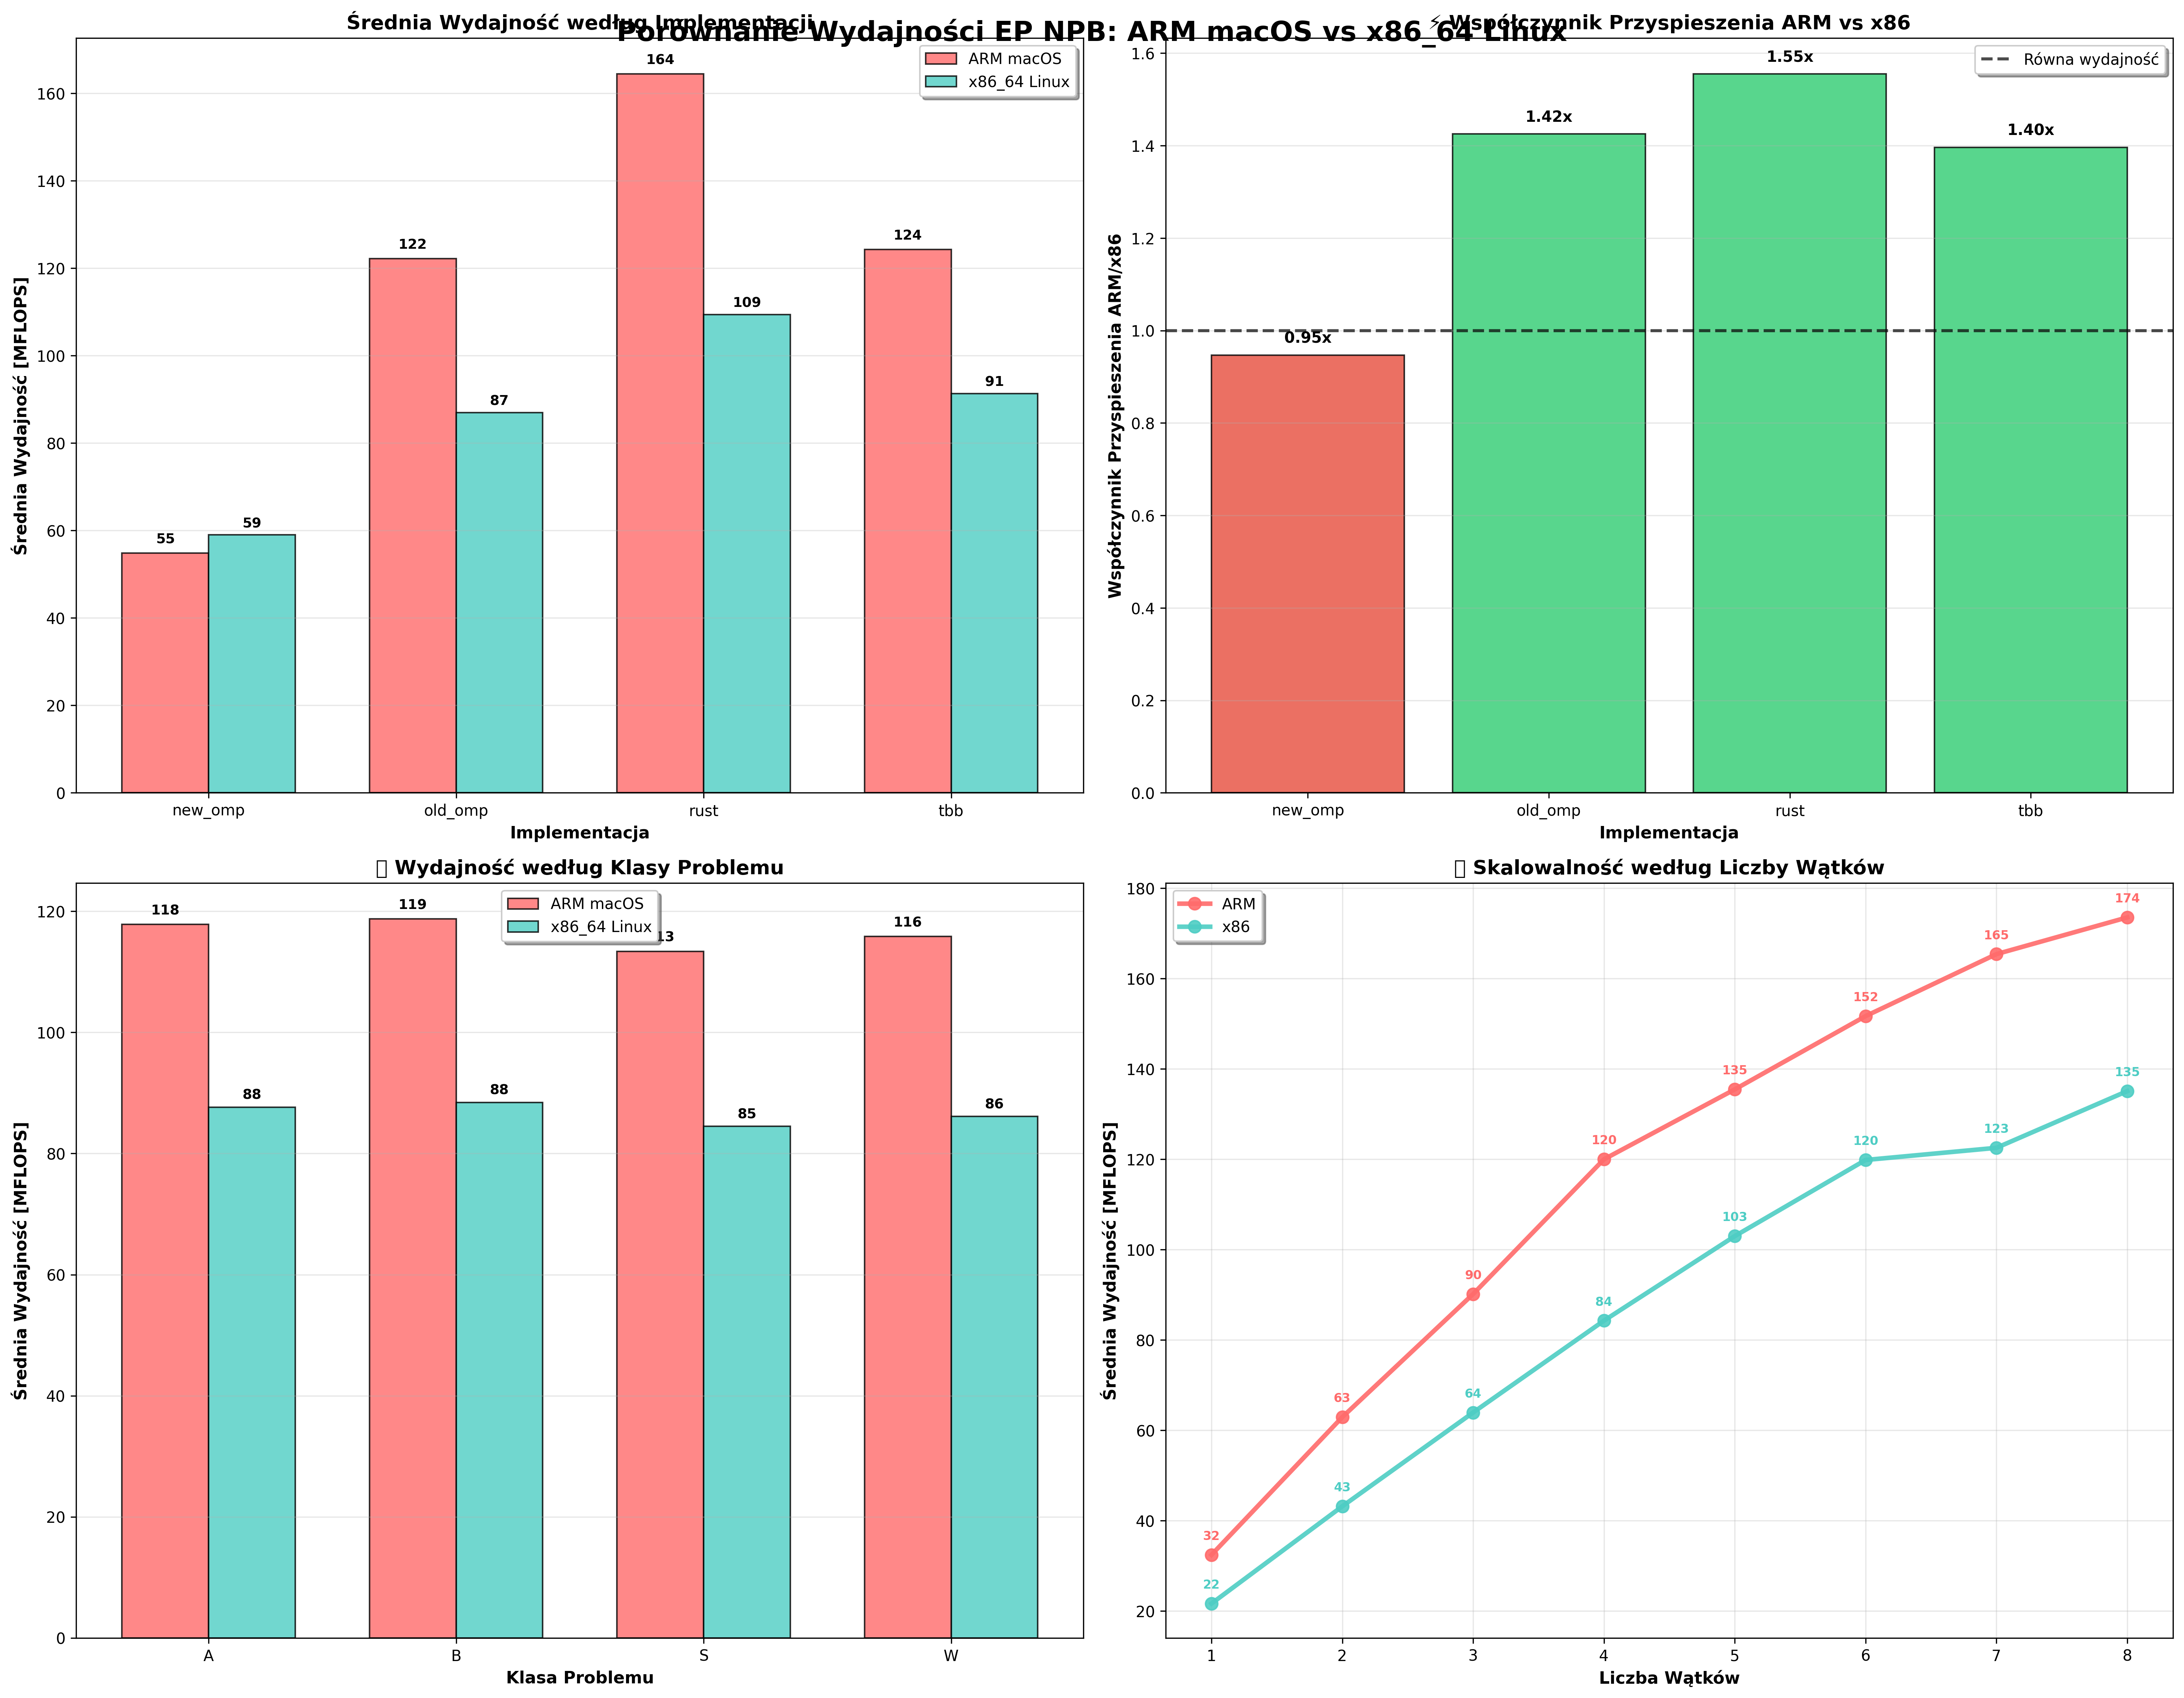
\includegraphics[width=0.9\textwidth]{analiza/images/parallel/ep/compare/ep_porownanie_platform_arm_vs_x86.png}
    \caption{Porównanie średniej wydajności benchmarku EP dla platform ARM64 i x86\_64}
    \label{ep_porownanie_platform_arm_vs_x86}
\end{figure}
\subsubsection{Porównanie wydajności według implementacji i architektury}
Analiza średnich wartości MFLOPS dla poszczególnych implementacji w podziale na platformy sprzętowe ujawnia wyraźne różnice, wskazujące na przewagę architektury ARM. Z wyjątkiem implementacji \texttt{new\_omp}, wszystkie rozwiązania osiągają wyższe wyniki na platformie \mbox{macOS} z~architekturą ARM. Szczególnie wyróżnia się implementacja \texttt{rust}, której średnia wydajność na ARM wynosi 164 MFLOPS w porównaniu do 109 MFLOPS na platformie x86\_64. Przewaga ta wynosi około 50\%, co wskazuje na bardzo dobrą adaptację tej implementacji do architektury ARM.

Na obu platformach to właśnie implementacja \texttt{rust} osiąga najwyższe wyniki, podczas gdy \texttt{new\_omp} pozostaje najwolniejszym wariantem. Warto zaznaczyć, że \texttt{new\_omp} jest jedyną implementacją, która uzyskuje nieco wyższą średnią wydajność na platformie x86\_64 (59 MFLOPS) niż na ARM (55 MFLOPS), co może świadczyć o ograniczonej optymalizacji tego rozwiązania pod kątem architektury ARM.

Współczynniki przyspieszenia obliczone jako stosunek średniej wydajności na ARM względem x86\_64 potwierdzają powyższe obserwacje. Najwyższy współczynnik (1,55x) notuje implementacja \texttt{rust}, natomiast \texttt{old\_omp} i \texttt{tbb} osiągają zbliżone wartości odpowiednio 1,42x i~1,40x. Jedyną implementacją z wartością poniżej jedności (0,95x) pozostaje \texttt{new\_omp}, co oznacza względnie słabsze skalowanie na ARM.

\subsubsection{Wydajność w zależności od klasy problemu}
Analiza wydajności w podziale na klasy problemowe, wykazuje spójną przewagę platformy ARM we wszystkich rozmiarach instancji. Dla każdej klasy problemowej wartości MFLOPS utrzymują się na zbliżonym poziomie, co sugeruje dobrą skalowalność algorytmu niezależnie od rozmiaru danych wejściowych. Średnie wartości dla platformy ARM mieszczą się w przedziale 118-119 MFLOPS, natomiast dla platformy x86\_64 wynoszą około 85-88 MFLOPS. Przewaga ARM w tym ujęciu wynosi około 35\%, co potwierdza, że jest to systemowo korzystniejsza architektura dla danego typu obciążeń obliczeniowych.


\subsubsection{Skalowanie według liczby wątków}
Wykresy prezentujące wydajność w zależności od liczby wątków ukazują zbliżone trendy dla obu architektur. W obu przypadkach obserwuje się niemal liniowy wzrost wydajności do poziomu 5-6 wątków, po czym przyrost staje się bardziej umiarkowany. Jest to zgodne z typowym zachowaniem dla aplikacji równoległych, w których narzuty synchronizacji i ograniczenia sprzętowe zaczynają odgrywać większą rolę przy dalszym zwiększaniu liczby wątków.

Pod względem wartości bezwzględnych platforma ARM osiąga wyższe maksima - przy 8 wątkach wydajność sięga około 174 MFLOPS, podczas gdy dla x86\_64 wynosi ona \mbox{135 MFLOPS}. Również ogólna efektywność skalowania jest nieco wyższa na ARM, choć analiza wykresów efektywności równoległej wskazuje na szybszy spadek tej metryki przy większej liczbie wątków. Dla ośmiu wątków efektywność na ARM spada do około 68\%, podczas gdy na x86\_64 utrzymuje się na poziomie około 78\%. Może to wskazywać na większą wrażliwość architektury ARM na narzuty związane z wielowątkowością.
\begin{figure}[H]
    \centering
    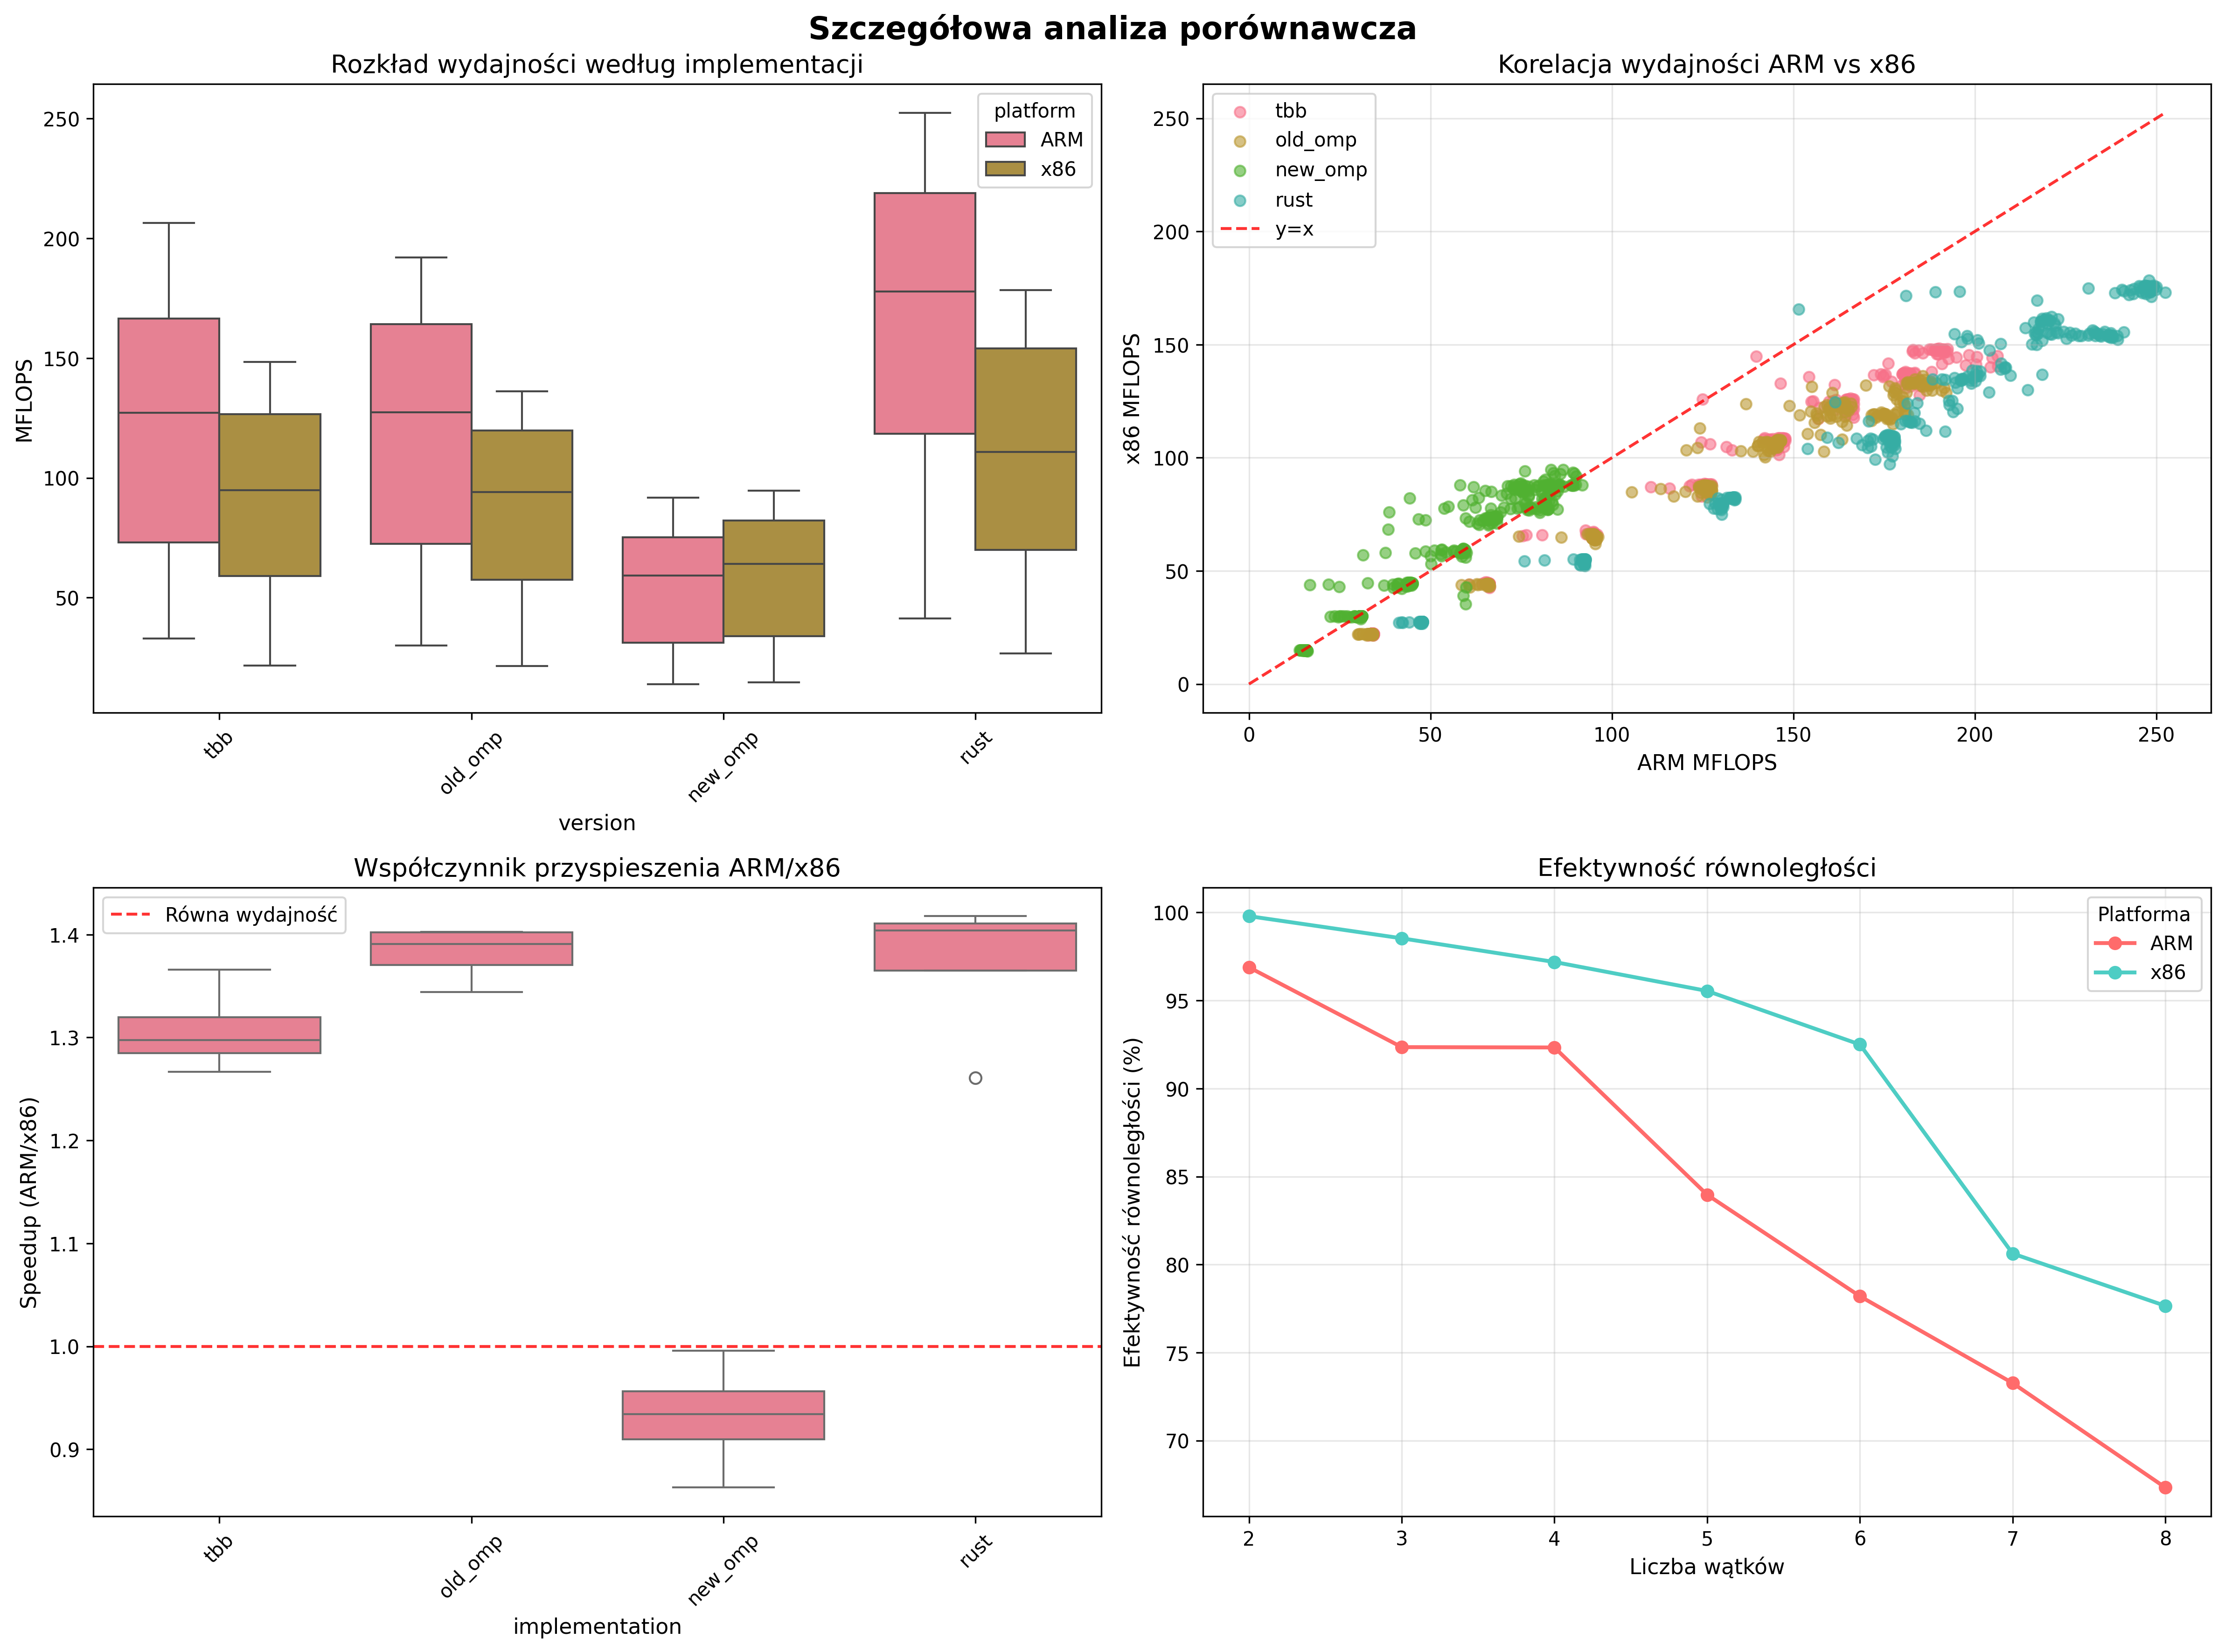
\includegraphics[width=0.9\textwidth]{analiza/images/parallel/ep/compare/ep_szczegolowa_analiza_wydajnosci.png}
    \caption{Szczegółowa analiza wydajności benchmarku EP dla platform ARM64 i x86\_64}
    \label{ep_szczegolowa_analiza_wydajnosci}
\end{figure}

Wyniki uzupełnia analiza rozkładów i korelacji wydajności dla obu platform - rysunek \ref{ep_szczegolowa_analiza_wydajnosci}. Wykresy pudełkowe dla implementacji \texttt{rust}, \texttt{old\_omp} oraz \texttt{tbb} pokazują wyraźne przesunięcie mediany i całego rozkładu ku wyższym wartościom na platformie ARM. Sugeruje to nie tylko wyższą średnią wydajność, ale także większą stabilność działania w zakresie typowych przypadków.

Wykres korelacji wydajności między platformami wskazuje na silną liniową zależność, przy czym większość punktów znajduje się wyraźnie powyżej linii y = x. Potwierdza to systematycznie wyższą wydajność ARM względem x86\_64, szczególnie w przypadku implementacji osiągających wysokie wartości MFLOPS.

\begin{figure}[H]
    \centering
    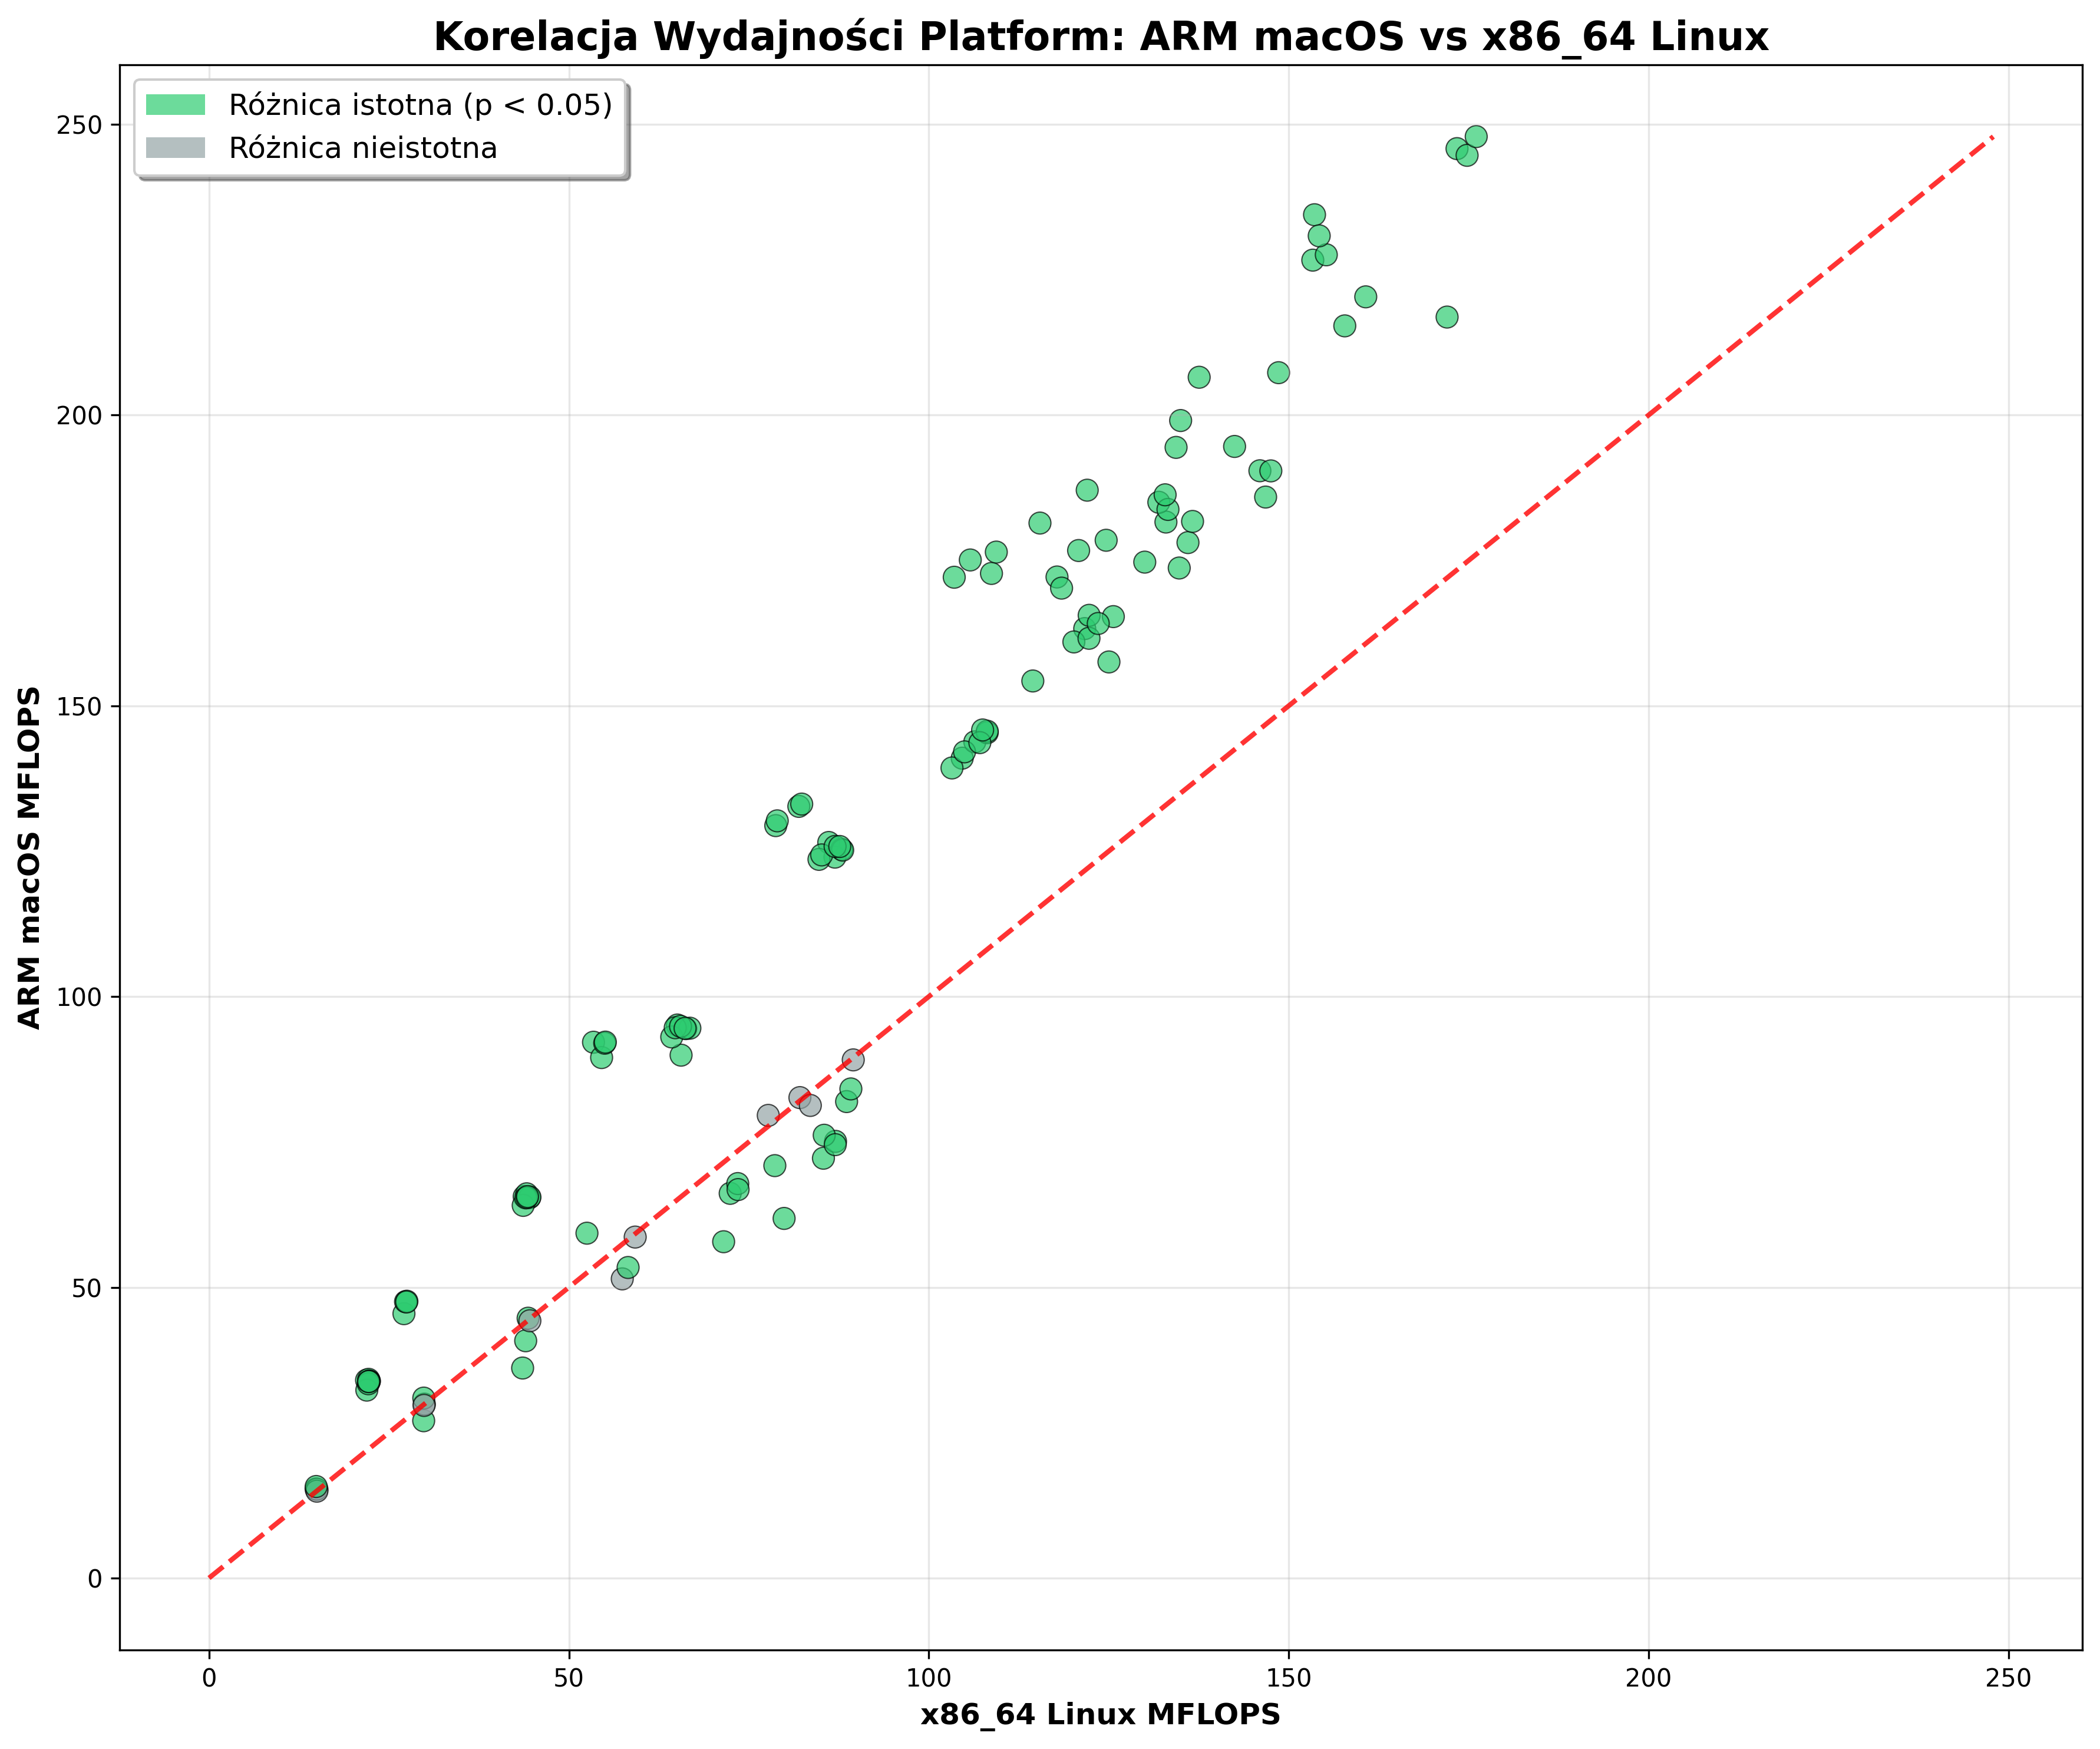
\includegraphics[width=0.9\textwidth]{analiza/images/parallel/ep/compare/ep_analiza_istotnosci_statystycznej.png}
    \caption{Analiza istotności statystycznej benchmarku EP dla platform ARM64 i x86\_64}
    \label{ep_analiza_istotnosci_statystycznej}
\end{figure}
Analiza statystyczna różnic wydajności - rysunek \ref{ep_analiza_istotnosci_statystycznej} wykazuje, że w zdecydowanej większości przypadków różnice te są statystycznie istotne (p < 0,05). Podnosi to wiarygodność wniosków oraz potwierdza, że zaobserwowane efekty nie są przypadkowe, lecz wynikają z realnych różnic architektonicznych i implementacyjnych.